% !TEX spellcheck = en-US

\documentclass[twoside,a4,12p]{report} %,draft,openright]

\usepackage{amsmath}%for equation split
\usepackage{mathalfa}%
\usepackage{epsfig}
\usepackage{graphicx}
\usepackage{float}
\usepackage{subfigure}
\usepackage{url}
\usepackage{color}

% define arg min 
\DeclareMathOperator*{\argmin}{arg\,min}

% Add psudeo-code 
\usepackage{algorithm}
\usepackage{algorithmic}
%\usepackage{algpseudocode}% http://ctan.org/pkg/algorithmicx
\makeatletter
\newcommand\fs@ruled@notop{\def\@fs@cfont{\bfseries}\let\@fs@capt\floatc@ruled

  \def\@fs@pre{}%
  \def\@fs@post{\kern2pt\hrule\relax}%
  \def\@fs@mid{\kern2pt\hrule\kern2pt}%
  \let\@fs@iftopcapt\iftrue}
\renewcommand\fst@algorithm{\fs@ruled@notop}
\makeatother
\restylefloat{algorithm}


\usepackage{latexsym,amssymb}
\usepackage{setspace,cite}
% for margins left, right top bottom
\usepackage{anysize}
\marginsize{4cm}{2.5cm}{4cm}{4cm}

\usepackage[pdftex,
  bookmarks=true,%                   %%% generate bookmarks ...
  bookmarksnumbered=true,%           %%% ... with numbers
  bookmarksopen=true,%               %%% show complete tree of bookmarks
  hypertexnames=true,%              %%% needed for correct links to figures !!!
  breaklinks=true,%                  %%% break links if exceeding a single line
  colorlinks=true,
  linkcolor=black,
  citecolor=blue,
  pagecolor=blue,
  pagebackref=false,
  urlcolor=blue]{hyperref}


%\usepackage{draft} %draft option - doesn't put full figures in -
            % useful when editing

%does the headers on the pages - keep in
\usepackage{fancyhdr}

%omitting any of these makes the thesis compile without the omitted
%chapter - good for editing single chapters.
%\includeonly{header,intro,background,appendix}

\begin{document}
\newpage

%Puts page numbering of preamble in roman and of main body of thesis in
%arabic. Also defines how chapters and sections are made
\pagenumbering{arabic}
\setcounter{page}{1} \pagestyle{fancy}
\renewcommand{\chaptermark}[1]{\markboth{\chaptername%
\ \thechapter:\,\ #1}{}}
\renewcommand{\sectionmark}[1]{\markright{\thesection\,\ #1}}

%DEFINES TITLE PAGE, and contains abstract, acknowledgements, etc.

%%%%%%%%%%%%%%%%%%%%%%%%%%%%%%%%%%%%%%%%%%%%%%%%%%%%%%%%%%%%%%%%%%%%%%%%%%%
% This is a sample header for a sample dissertation. Fill in the name,
% and the other information. LaTeX will work out the table of
% content, the list of figures and of tables for you.
%%%%%%%%%%%%%%%%%%%%%%%%%%%%%%%%%%%%%%%%%%%%%%%%%%%%%%%%%%%%%%%%%%%%%%%%%%%

\newpage
\thispagestyle{empty}

% ******* Title page *******
% **************************

\vspace*{-2cm}
\begin{center}
{\LARGE\bf High Quality Depth Refinement with Color Photometric Stereo\\} \vspace{2cm} {\Large \textbf{Songyou Peng}}\\
\vspace{1.5cm}
{
\large 
Supervised by:\\ \vspace{0.4cm}
 Dr. Yvain Qu\'eau \hspace{0.8cm} Prof. Daniel Cremers
}
\\\vspace{0.8cm}
{

\includegraphics[height=0.15\textheight]{figures/tum_logo.jpg}
\\\vspace{0.8cm}
\large
Computer Vision Group \\
\vspace{0.4cm}
Department of Computer Science\\
\vspace{0.4cm}
Technical University of Munich}

\end{center}

\vspace{2cm}
\begin{center}
{

\includegraphics[height=0.1\textheight]{figures/vibot_logo_transparent.png}
\\
\large A Thesis Submitted for the Degree of \\MSc Erasmus Mundus
in Vision and Robotics (VIBOT) \\\vspace{0.3cm} $\cdot$ 2017
$\cdot$}
\end{center}
\singlespacing


%ABSTRACT
\begin{abstract}
The abstract will go here....

\vspace*{5cm}



\begin{center}
\begin{quote}
\it Research is what I'm doing when I don't know what I'm
doing.\,\ldots
\end{quote}
\end{center}
\hfill{\small Werner von Braun}

\end{abstract}

\doublespacing

%\pagestyle{empty}
\pagenumbering{roman}
\setcounter{page}{1} \pagestyle{plain}


\tableofcontents

\listoffigures
\listoftables

\chapter*{Acknowledgments}
\addcontentsline{toc}{chapter}
         {\protect\numberline{Acknowledgments\hspace{-96pt}}}

Leave this part until I finish the whole thesis

\pagestyle{fancy}


\newpage

%sets up headers for lefthand and righthand pages. To alter, edit
%these lines and the chaptermark/sectionmark lines above
\addtolength{\headheight}{3pt} \fancyhead{}
\fancyhead[LE]{\sl\leftmark} \fancyhead[LO,RE]{\rm\thepage}
\fancyhead[RO]{\sl\rightmark} \fancyfoot[C,L,E]{}
\pagenumbering{arabic}

%\singlespacing
%\doublespacing
\onehalfspacing
\chapter{Introduction} \label{chap:intro}

\section{Preparing your dissertation} \label{sect:thefirst}

You are strongly encouraged to use the Latex templates provided.

\subsection{Paper}
The manuscript should be in A4 size, and the printed paper should
be of at least 70 gsm.

\subsection{Font and margins}
Thesis should be printed on both sides of the paper. Use no less
than 1.5 spacing, with quotations and notes single-spaced.
Regarding \textbf{Character size}, not less than 2.0mm for
capitals and 1.5mm for x-height (the height of a lower-case x). Us
a serif font (i.e. Times) between 10 and 12 points. Use consistent
and clear fonts through all the document.

The text layout should be approximately as follows:

\begin{itemize}
    \item $4cm$ binding margin
    \item $2cm$ head margin (top of page)
    \item $2.5cm$ fore-edge margin
    \item $4cm$ tail margin (bottom of page)
\end{itemize}

\section{Title Page}
The title page should contain the title of thesis, authors name,
and at the foot of the page: the name of degree,  Your University,
and the year of presentation. Something like this:

\vspace*{1cm}
\begin{center}
{\Large\bf MSc. Thesis example VIBOT\\} \vspace{2cm} {\large
Robert Mart\'i\\
\vspace{1cm}
Department of Computer Architecture and Technology \\
University of Girona}

\end{center}

\vspace{2cm}
\begin{center}
{\large A Thesis Submitted for the Degree of MSc Erasmus Mundus in
Vision and Robotics (VIBOT)\\ \vspace{0.3cm} $\cdot$ 2008 $\cdot$}
\end{center}


\subsection{References}
You can reference other authors by using the $cite command$
\cite{Pokorski:1998hr}. You are encouraged to use bib files and
let bibtex do the job for you.

\chapter{Background} \label{chap:background}
%%%%%%%%%%%%%%%%%%%%%%%%%%%%%%%%%%%%%%%%%%%%
\section{RGB-D Cameras}
%%%%%%%%%%%%%%%%%%%%%%%%%%%%%%%%%%%%%%%%%%%%

%----------------------------------------------
\subsection{General}
%----------------------------------------------
RGB-D cameras have been widely used in many modern computer vision areas, for example 3D reconstruction~\cite{newcombe2011kinectfusion}, visual odometry and mapping on quadrocopter~\cite{huang2017visual} and visual SLAM algorithms~\cite{engelhard2011real}. 
A RGB-D camera returns a color image which is usually in RGB color space, and a depth map, every pixel of which reflects the real-world distance between the camera and the corresponding position of the pixel.
Depending on the technologies used to measure the depth information, the RGB-D camera can be divided to passive and active~\cite{kerl2012msc}.

The so called passive RGBD-camera usually contains two RGB cameras with a known translation between them.
After taking one picture for each, the features in two pictures are matched and then the triangulation is applied to obtain the depth.
An illustration is shown in Fig.~\ref{fig:rgbd_camera_passive}.

Active technologies usually emit lights to the environment so it has the capability of acquiring depth images in a totally dark indoor scenario.
They can be furthered categorized as time of flight (ToF) or structured light approaches.

A ToF camera calculates the depth in each pixel by measuring the delay between the emission and the reflected time.
ToF cameras typically emit either pulsed light or modulated light.
The Microsoft Kinect 2.0 and IFM Efector are two examples of the ToF camera.

The RGB-D cameras with the structured light use a projector for a known pattern. 
Since the transformation between the camera the projector is pre-given, a camera observes the projected pattern and then triangulates to calculate the depth (Fig.~\ref{fig:rgbd_camera_active}).
The ASUS Xtion Pro Live, Intel RealSense R200 and Ensenso are several well-known cameras using structured lights.
It should be noted that many active stereo cameras project infrared (IR) lights. 
Due to the fact that sun is a source of infrared lights, the usage of these cameras is limited to the indoor environment.


\begin{figure}[!htbp]
\centering
\subfigure[Passive stereo]{\label{fig:rgbd_camera_passive} 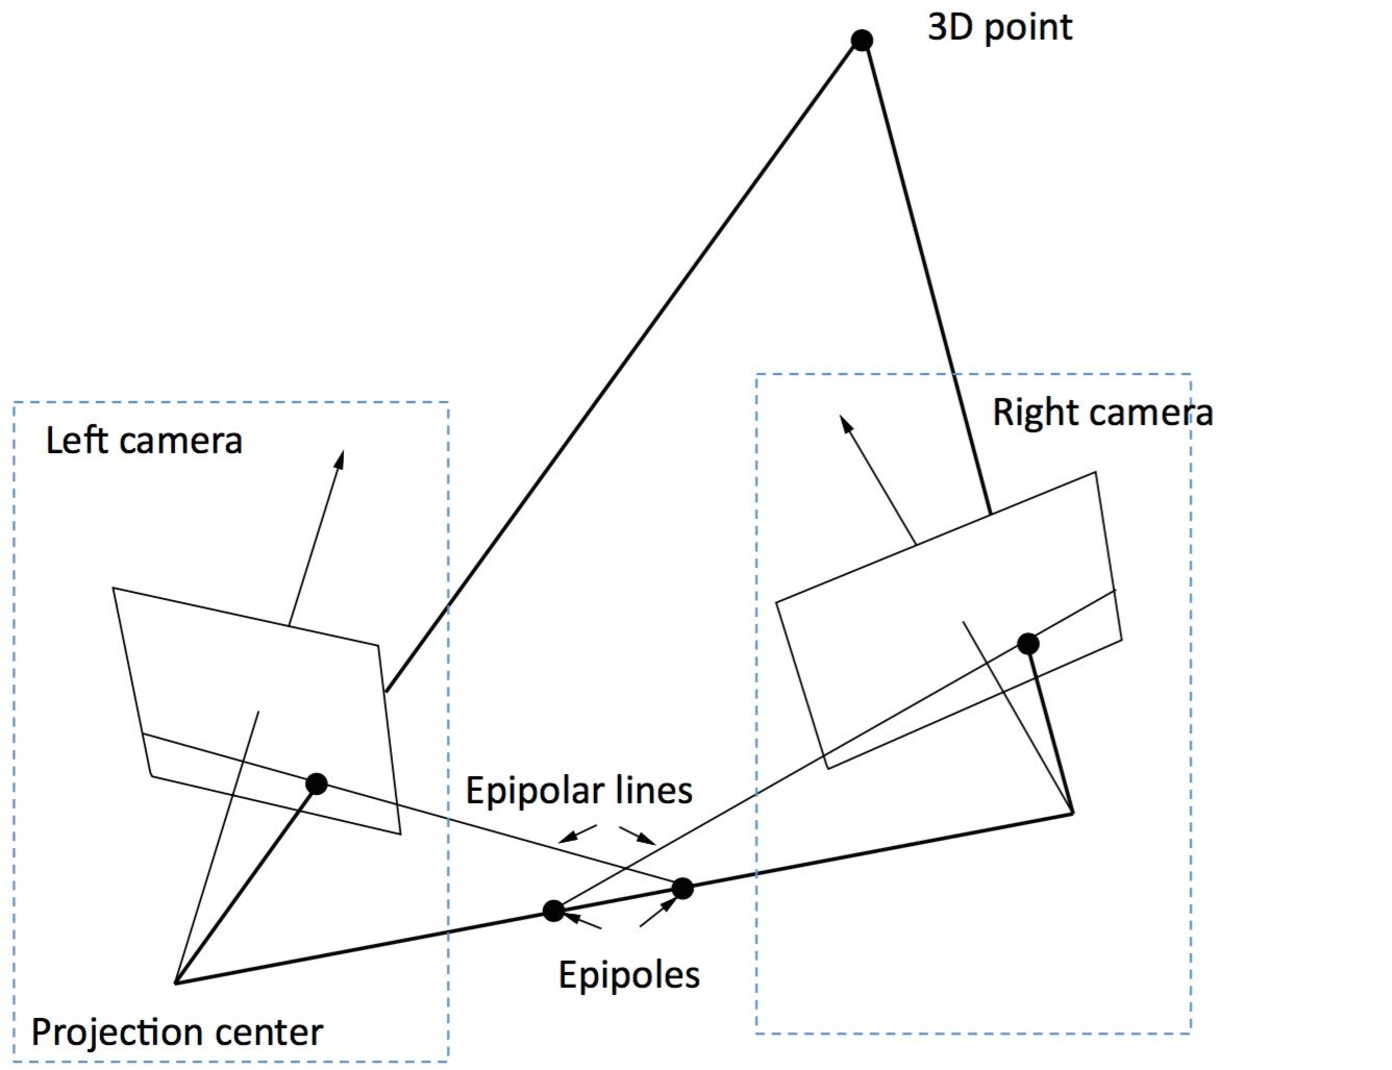
\includegraphics[width=0.40\linewidth]{figures/camera_passive.pdf}}
\subfigure[Active stereo]{\label{fig:rgbd_camera_active} 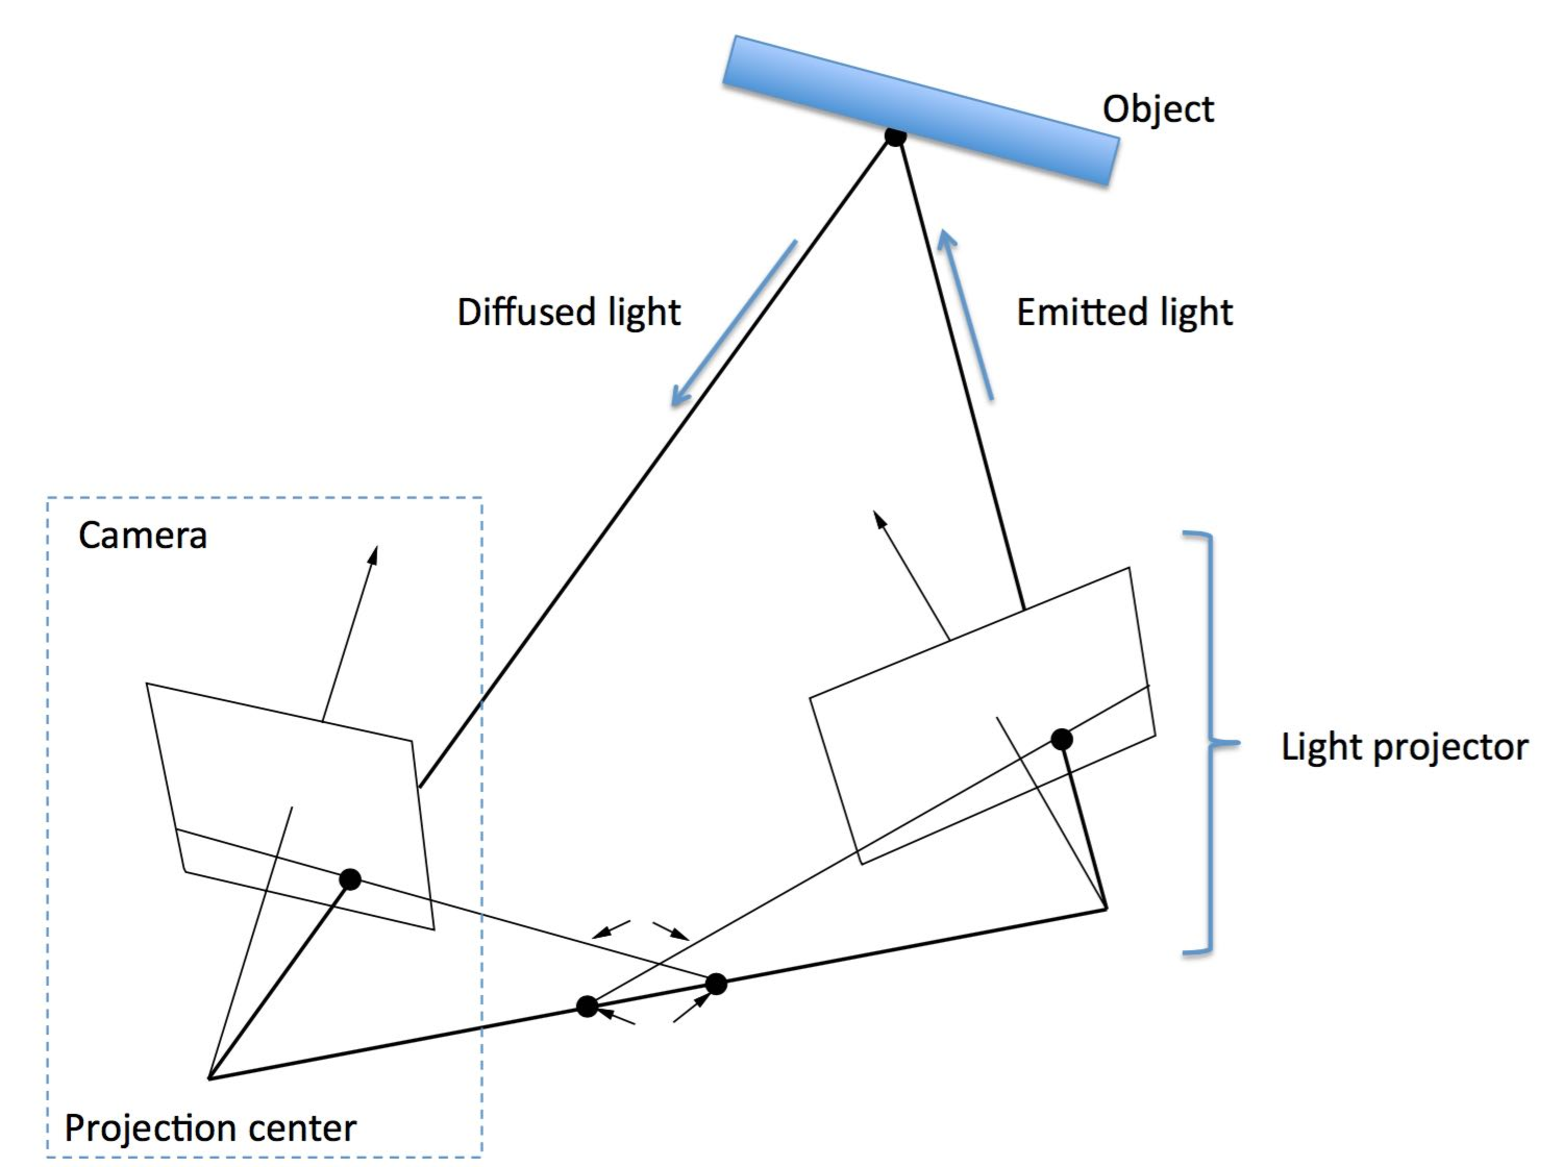
\includegraphics[width=0.45\linewidth]{figures/camera_active.pdf}}
\caption{Illustrations for the principle of passive and active stereo. Image courtesy of~\cite{horaud2013tutorial}.}
\label{fig:rgbd_camera}
\end{figure}


%%%%%%%%%%%%%%%%%%%%%%%%%%%%%%%%%%%%%%%%%%%%
\subsection{ASUS Xtion PRO LIVE}
%%%%%%%%%%%%%%%%%%%%%%%%%%%%%%%%%%%%%%%%%%%%

\begin{figure}[!ht]
\centering
\subfigure[Camera structure~\cite{asus}]{\label{fig:asus_structure} 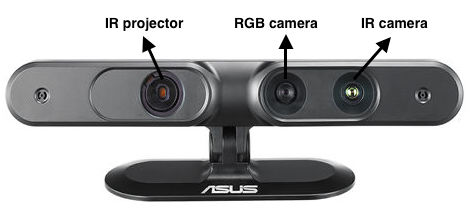
\includegraphics[width=0.4\linewidth]{figures/asus.jpg}}\\
\subfigure[RGB image]{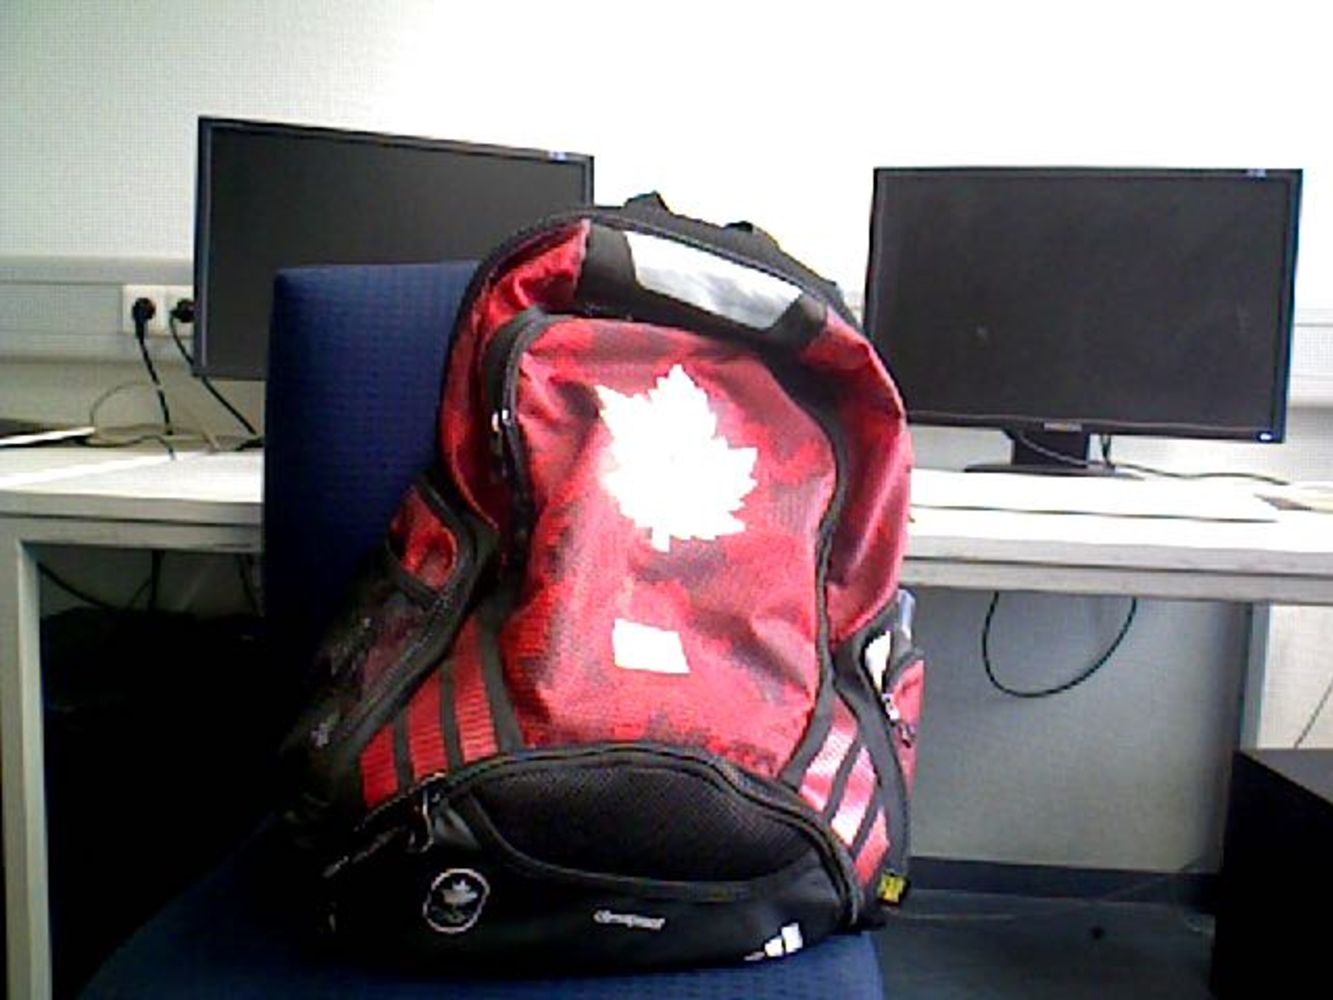
\includegraphics[width=0.4\linewidth]{figures/scene_rgb.pdf}}
\subfigure[Depth image]{ 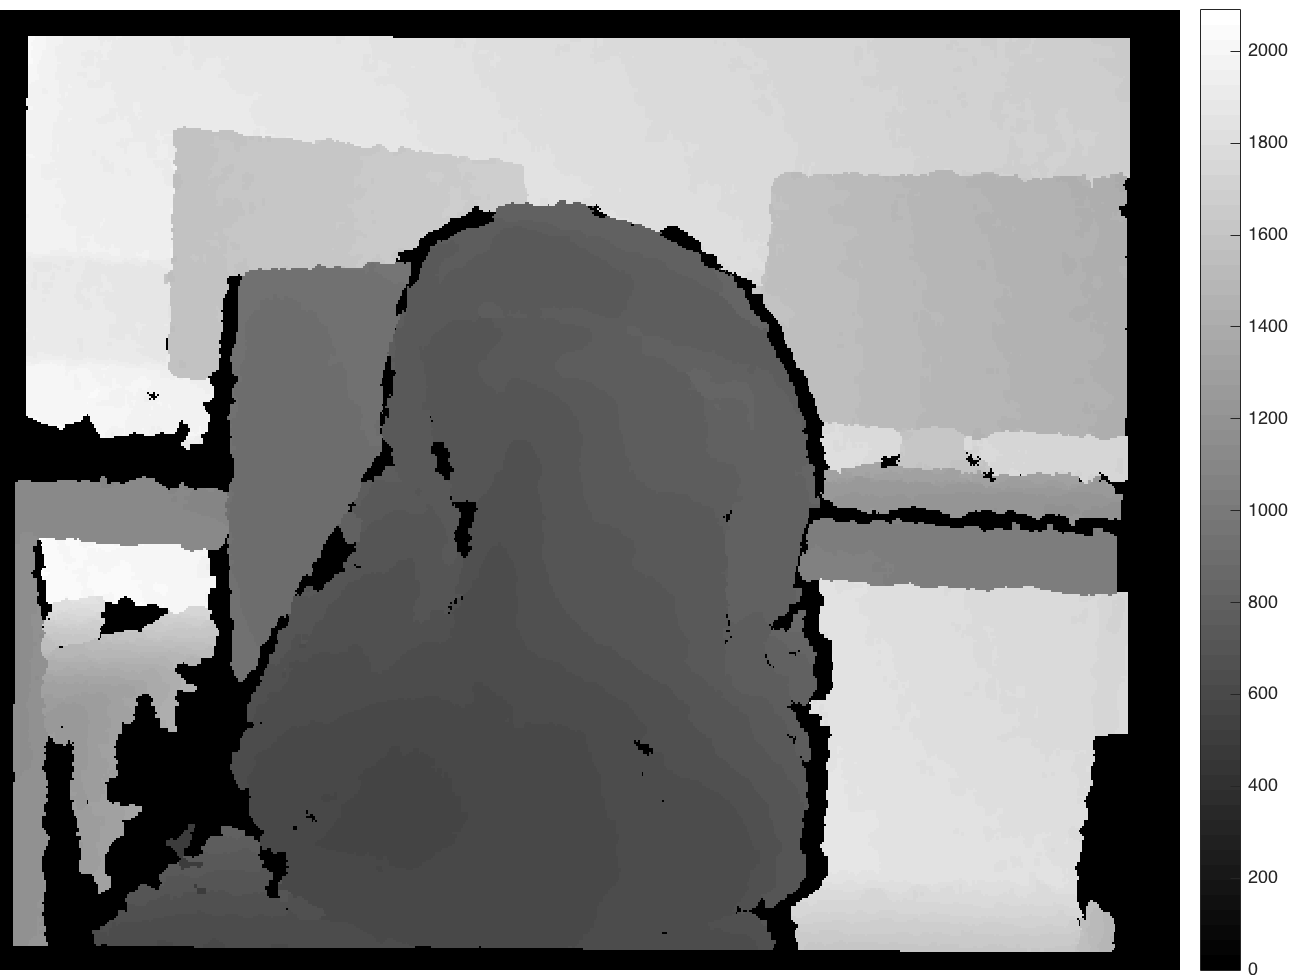
\includegraphics[width=0.4\linewidth]{figures/scene_depth.png}}
\caption{Upper row: the structure of ASUS Xtion Pro Live. Lower row: the RGB and depth images of an indoor scene acquired by this RGB-D camera. The unit in (c) is millimetre.}
\label{fig:asus_illustration}
\end{figure}
The ASUS Xtion Pro Live camera has two cameras and an IR projector as shown in Fig.~\ref{fig:asus_structure}.
According to the official website~\cite{asus}, it provides the RGB image with the maximum resolution of $1280\times1024$, while the depth can be alternated either VGA resolution ($640\times480$ with 30fps) or QVGA ($320\times240$ with 60fps). 
Its depth is reported to range from 0.8 to 3.5m, but we found in the experiments that the blind area was less and merely around 0.5m.  
Xtion Pro Live has been used throughout our experiments and we choose different configurations depending on the applications.
When the depth super-resolution is required, the RGB images have the resolution of $1280\times1024$, otherwise we keep the same RGB resolution as the depth ($640\times480$).

%%%%%%%%%%%%%%%%%%%%%%%%%%%%%%%%%%%%%%%%%%%%
\section{Shape from Shading \& Photometric Stereo}

The well-known shape from shading (SFS) problem was first introduced by Horn~\cite{horn1970shape} in 1970 and then a large amount of literature flooded in to develop the field.
The idea of SFS is, knowing the light source position, one can estimate the shape or the surface of an object from one single grayscale image.
This inverse problem is highly ill-posed, as illustrated in Fig.~\ref{fig:paint}.


\begin{figure}[!ht]
\centering
\subfigure[An image]{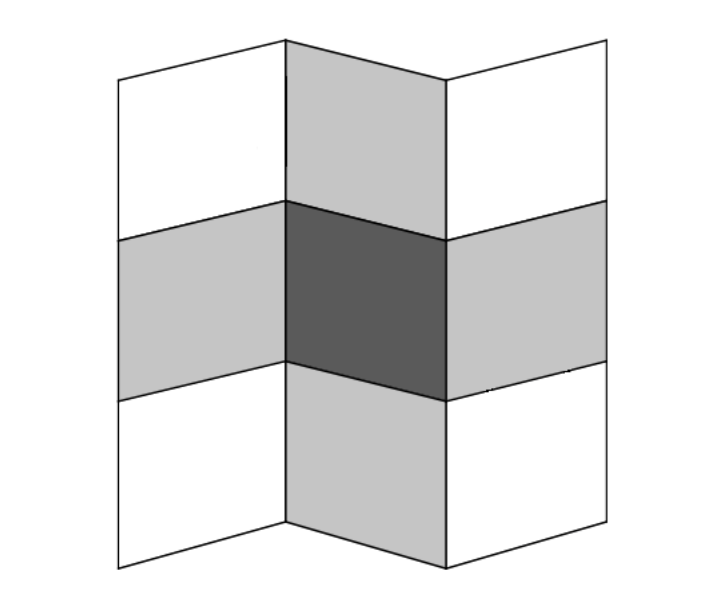
\includegraphics[width=0.25\linewidth]{figures/paint.png}}
\subfigure[A possible explanation~\cite{barron2015shape}]{ 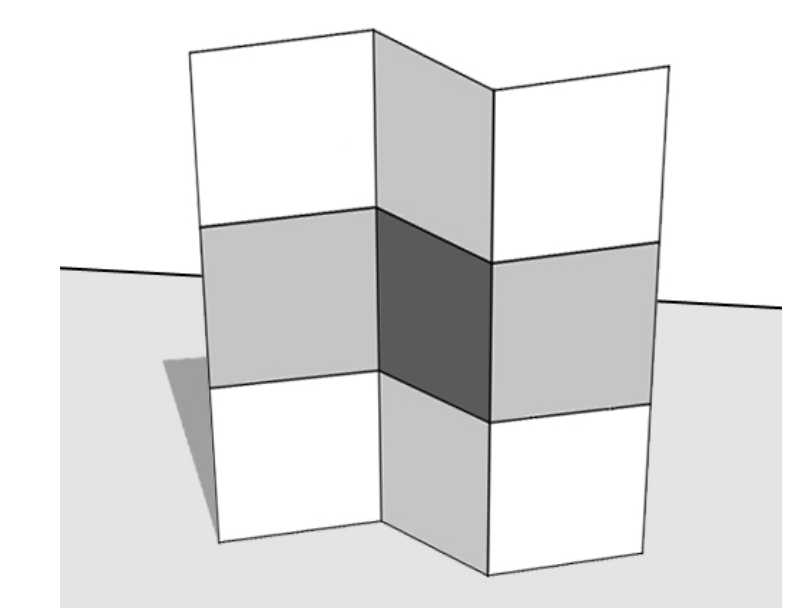
\includegraphics[width=0.3\linewidth]{figures/paint0.png}}\\
\subfigure[painter's explanation]{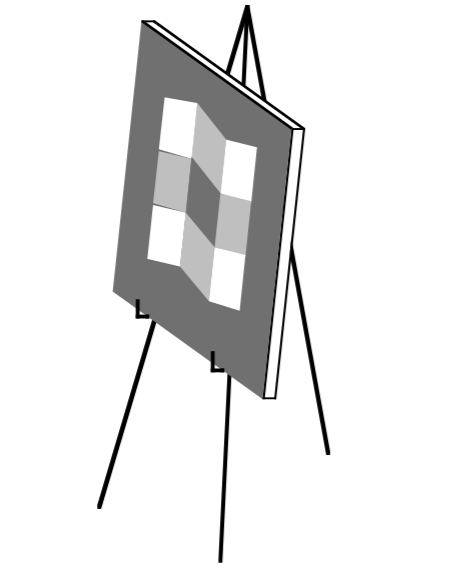
\includegraphics[width=0.2\linewidth]{figures/paint1.png}}
\subfigure[sculptor's explanation]{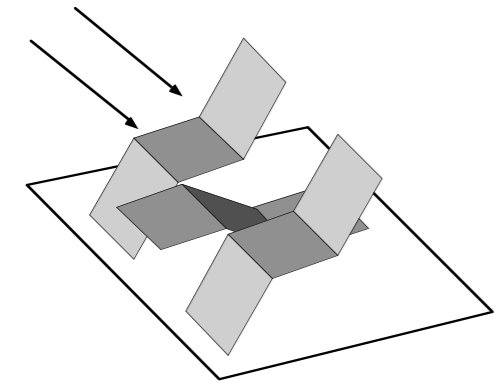
\includegraphics[width=0.3\linewidth]{figures/paint2.png}}
\subfigure[Lighting designer's explanation]{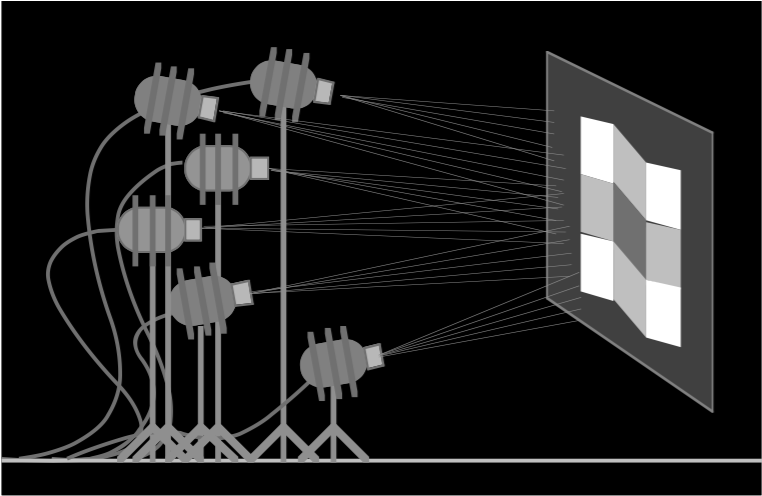
\includegraphics[width=0.3\linewidth]{figures/paint3.png}}
\caption{Various explanations for a twice-bent surface. Illustrations for the ambiguity suffered by SFS. Images courtesy of~\cite{adelson1996perception}.}
\label{fig:paint}
\end{figure}


From the mathematical perspective, the luminance can be separated as follows:
\begin{equation}\label{eq:sfs_equation}
    I = \rho S
\end{equation}
where $I$ is an intensity image, $\rho$ is the reflectance (albedo) of the surface, and the $S$ is the shading image. 
An example of such an image decomposition is shown in Fig.~\ref{fig:shading}.
%&&&&&&&&&&&&&&&&&&&&&&&&&
\begin{figure}[!htbp]
\centering
\setlength{\tabcolsep}{0.1em} % column spacing
 {\renewcommand{\arraystretch}{0.6}% row spacing
\begin{tabular}{c c c c c}
   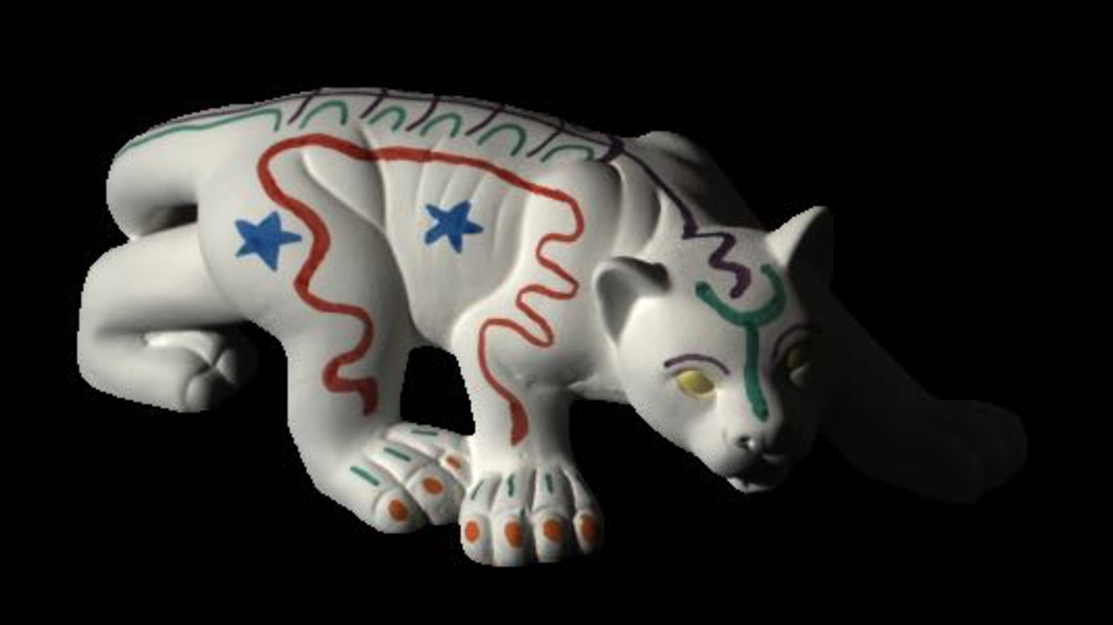
\includegraphics[height = 0.16\linewidth]{figures/panther_rgb.pdf} \hspace{0.05cm}   &
   \multirow{-10}{*}{\parbox[t]{3.5mm}{=}}  & 
   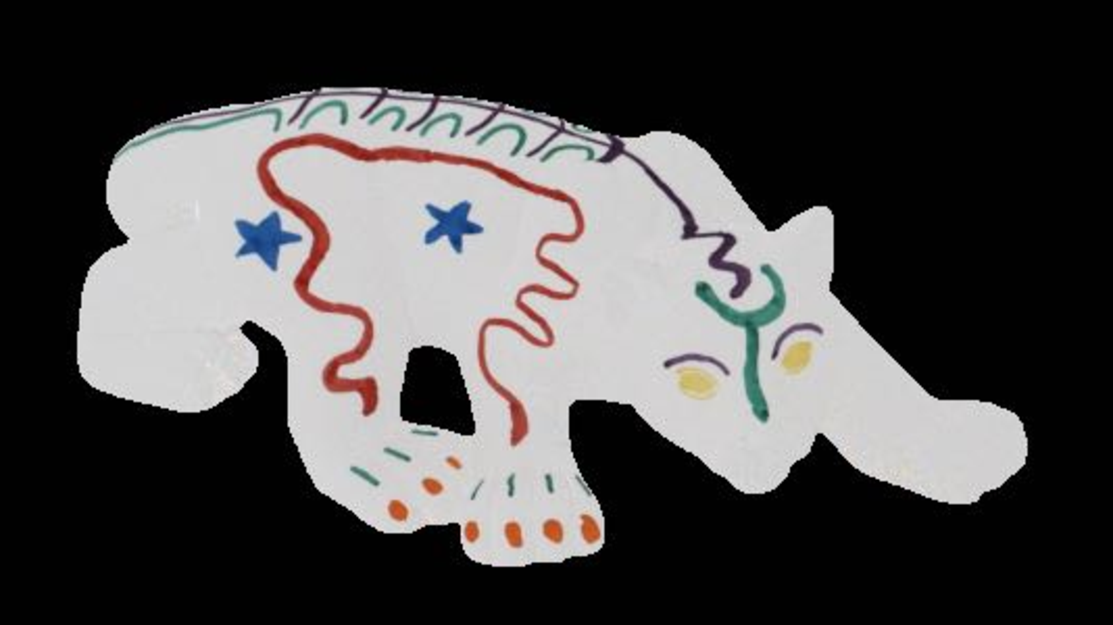
\includegraphics[height = 0.16\linewidth]{figures/panther_rho.pdf} &
    \multirow{-10}{*}{\parbox[t]{3.5mm}{$\times$}}  & 
   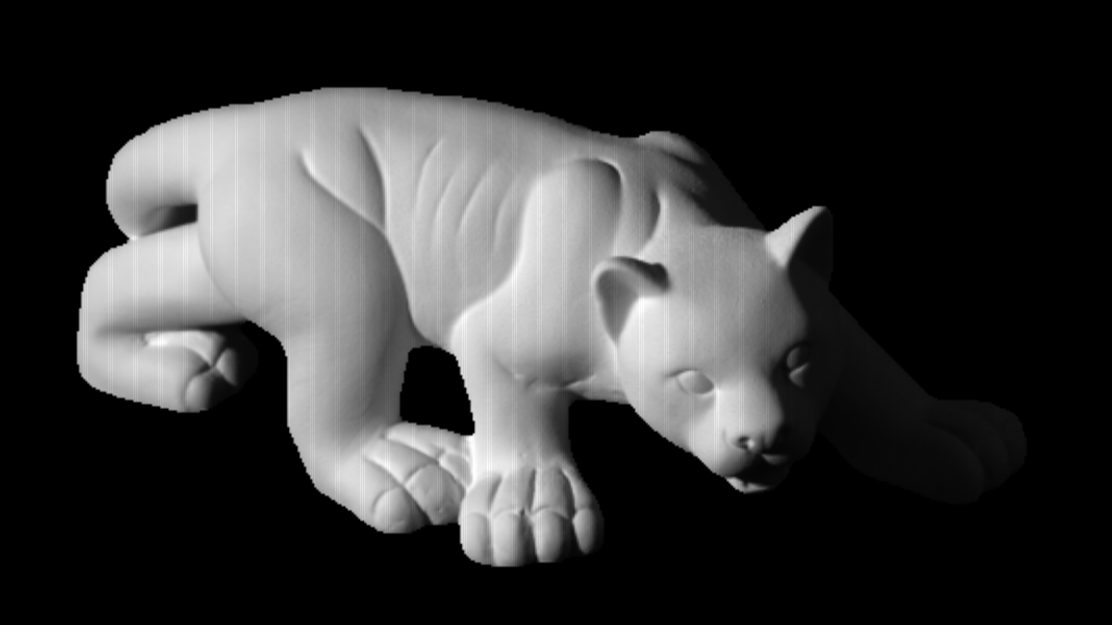
\includegraphics[height = 0.16\linewidth]{figures/panther_shade.pdf} \\
      {I} &{} &{$\rho$} & {}& {$S$}            
 \end{tabular}}
\caption{The decomposition of a color image of a toy panther. $\rho$ is the reflectance (albedo) and $S$ is the shading. Images are from MIT intrinsic images dataset~\cite{grosse2009ground}.}
\label{fig:shading}
\end{figure}
%&&&&&&&&&&&&&&&&&&&&&&&&&

SFS approches assume the observed object follows the Lambert's cosine law~\cite{klett1760ih}, based on which the Eq.~\ref{eq:sfs_equation} can be reformulated to the Lambertian reflectance model:
\begin{equation}\label{eq:lambertian_model}
    I = \rho \; \mathbf{l}^\top \mathbf{n}
\end{equation}
where we can notice that the shading $S$ is the inner product of the light direction and the surface normal.
Thus, the task of SFS is to retrieve the shape (surface normal) from the shading based on the Lambertian reflectance model.
Moreover, many state-of-the-art shape or depth refinement methods used an extension of Lambertian model called spherical harmonics (SH) \cite{basri2003lambertian, ramamoorthi2001relationship} which can represent the illumination more realistically. 
It has been shown that the first-order SH model (Eq.~\ref{eq:sh_model}) can account for $87.5\%$ of real world light so we applied it throughout the whole thesis:
\begin{equation}\label{eq:sh_model}
    I = \rho \; (\mathbf{l}^\top \mathbf{n} + \varphi)
\end{equation}
where $\varphi$ can be understood as the ambient light parameter.

The goal of SFS is to estimate the shape or the surface of object, which is represented by the surface normal $\mathbf{n}$.
Two camera projection models are usually used for modelling the surface normal: orthographic and perspective projection.
To derive $\mathbf{n}$ using orthographic projection, we consider projection along the $z$-axis\cite{hartley2003multiple}.
Hence, A 3D point $P = (x,y,z)$ is mapped to the image point $p = (x,y)$.
It should be noted that the depth $z$ depends on the coordinate $x$ and $y$.
And we know the surface normal is orthogonal to the tangent plane in $(x,y)$, which can be written as:
\begin{equation}
    \mathbf{n}(P) \propto \; \partial_x P \times \partial_y P 
    = \begin{pmatrix} 1 \\ 0 \\ z_x\end{pmatrix}
    \times \begin{pmatrix} 0 \\ 1 \\ z_y\end{pmatrix}
    = -\begin{pmatrix} z_x \\ z_y \\ -1\end{pmatrix}
\end{equation}
After normalizing and choosing the outward direction, we acquire the unit-length surface normal with orthographic projection:
\begin{equation}
    \mathbf{n}_{ortho} = \frac{1}{\sqrt{|\nabla z| + 1}} \begin{pmatrix} \nabla z \\ -1\end{pmatrix}
\end{equation}
For the more realistic perspective model, the 3D point $P$ now becomes $\begin{pmatrix} (x - x_0)/f \\ (y - y_0)/f\\ z\end{pmatrix}$ and the corresponding normal is:
%$$$$$$$$$$$$$$$$
\begin{equation}\label{eq:ratio_normal}
    \mathbf{n}_{perspect} =
    \frac{1}{d}
     \begin{pmatrix}
         f\tilde{z}_x\\
         f\tilde{z}_y\\
         -1 - (x-x_0)\tilde{z}_x - (y - y_0)\tilde{z}_y
     \end{pmatrix}
\end{equation}
%$$$$$$$$$$$$$$$$
where $\tilde{z} = \log{z}$, $f$ the focal length, $(x_0, y_0)$ the coordinates of principle points, and the normalizer $d =  \sqrt{(f\tilde{z}_x)^2 + (f\tilde{z}_y)^2 + (-1 - (x-x_0)\tilde{z}_x - (y - y_0)\tilde{z}_y)^2}$.

From the definition of the surface normal, we can notice the SFS is an ambiguous problem. 
Even when the lighting and the albedo are known in Eq.~\ref{eq:lambertian_model}, the inverse problem is ill-posed because the normal has 2 degrees of freedom. 
As we can see from Fig.~\ref{fig:paint}, the solution of SFS is ambiguous.
Horn and Brooks~\cite{horn1986variational} proposed the so-called integrability constraint $z_{xy} = z_{yx}$, which was the first constraint imposed on surface normal to make the SFS problem well-posed. 
Frankot and Chellapa~\cite{frankot1988method} projected a non-integrable surface to the subspace spanning the valid smooth surface.


Provided we have several images from the same view but with different illuminations, Eq.~\ref{eq:sfs_equation} can be modelled as:
\begin{equation}\label{eq:ps_equation}
    \mathbf{I = BL}
\end{equation}
Assuming there are $n \geqslant 3$ images from various illumination conditions, with $m$ pixels in each image, $\mathbf{I}\in \mathbb{R}^{m\times n}$ is the stack of all the intensity images and each column of $\mathbf{I}$ represents a vectorized image from a lighting condition.
 $\mathbf{B}\in\mathbb{R}^{m\times3}$ corresponds to $\rho \boldsymbol{\cdot} \mathbf{n}^\top$ and $\mathbf{L}\in\mathbb{R}^{3\times n}$ represents $ n$ various lightings.
If the illuminations are known, we call this problem \emph{calibrated} photometric stereo (PS), which was first introduced by Woodham~\cite{woodham1980photometric} in 1980. The problem is over-constrained so the surface normals can be estimated using a simple least squares. 
Some regions may sometimes suffer from the shadows for a certain illumination, so Forsythe and Ponce~\cite{forsyth2003modern} formed a diagonal matrix to eliminate all those shadow points.
Another interesting example of calibrated PS was proposed by Hern{\'a}ndez \emph{et al.}~\cite{hernandez2011overcoming}.
They controlled red, green, and blue lights from three directions and acquired the shape from only one color image, every channel of which was treated as a separate intensity image.   
This was one of the inspiration of our first proposed method RGB ratio model, which will be detailed in chapter~\ref{chap:methodology}.

However, the different lightings are not always controlled or given, then we call this kind of problem \emph{uncalibrated} photometric stereo. 
Hayakawa~\cite{hayakawa1994photometric} found that the surface normals and the albedo could be recovered with a $3\times3$ linear transformation using singular value decomposition. Yuille and Snow~\cite{yuille1997shape} further reduced the ambiguity to a gerenalized bas-relief (GBR) ambiguity by adding the integrability constraint. Now Eq.~\ref{eq:ps_equation} can be represented as
\begin{equation}\label{eq:ps_gbr}
    \mathbf{I} = \mathbf{B}\mathbf{A}^{-1}\mathbf{A}\mathbf{L}    
\end{equation}
where $\mathbf{A}$ is the GBR matrix:
\begin{equation}
    \mathbf{A} = 
    \begin{pmatrix}
        1& 0 & 0\\
        0& 1 & 0\\
        \mu & \nu & \lambda
    \end{pmatrix}
\end{equation}

There is a large amount of research work trying to solve the GBR ambiguity in uncalibrated PS.
Alldrin \emph{et al.}~\cite{alldrin2007resolving} used the prior emphasizing that the albedo distribution should have a low entropy, to resolve the ambiguity.
Favaro and Papadhimitri~\cite{papadhimitri2014closed} eliminated the ambiguity by exploiting the spatial maximum points of the inner product between the normals and the lights.
They also found out the solution is unique when the normal is constructed under the perspecitve projection instead of the orthographic projection~\cite{papadhimitri2013new}.
Qu\'{e}au \emph{et al.}~\cite{queau2015solving} estimated the GBR parameters by imposing the total variation norm.

In terms of depth, the GBR ambiguity is equivalent to the equation~\cite{belhumeur1999bas}:
\begin{equation}
    z(x,y) = \lambda z(x,y) + \mu x + \nu y
\end{equation}
Based on the equation, we find out that the GBR ambiguity still exists for the task of depth estimation.
However, since the rough depth will be given as the input from RGB-D camera, the GBR ambiguity problem encountered by uncalibrated PS is resolved automatically.
%Two examples about GBR ambiguity can be seen in Fig.~\ref{fig:ps_comp_syn} and~\ref{fig:ps_comp}.
Therefore, we will discuss some state-of-the-art depth refinement approaches.

 

\section{Depth and Shape Refinement}
%%%%%%%%%%%%%%%%%%%%%%%%%%%%%%%%%%%%%%%%%%%%

In recent years, there is a large amount of literature focusing on the depth or shape refinement based on either SFS (only use one single image) or PS (multiple images with different illuminations).
They are collectively called shading-based methods.
We will discuss these two streams respectively in the following.
%----------------------------------------------
\subsection{SFS-based methods}
%----------------------------------------------
Since SFS iteslf uses only one input image, it suffers from some intrinsic ambiguities that we have mentioned in the last section even when the light and the albedo are specified, so there will be more than one possible solution.
Now, although a rough depth map is given, the illumination and the albedo are unknown, so some regularization terms have to be imposed in order to acquire an exact solution from the inverse problem.

Han \emph{et al.}~\cite{han2013high} presented a framework which combines a global lighting model using the given color and depth with the help of SH model, with a local lighting model which varies spatially. 
The surface orientations should obey the integrability constraint on the smooth surface so they enforced the constraint by penalizing the curl of local neighborings.
However, the albedo in their method is assumed to be uniform.
To handle the multi-albedo objects, they had to apply another intrinsic image decomposition algorithm~\cite{barron2011high} and k-mean clustering to group the albedos into some areas with constant values inside.
Such framework is not only unrealistic but also very time-consuming so not able to be adapted to the real-world applications.

Yu \emph{et al.}~\cite{yu2013shading} iteratively update SH lighting and the albedo using the initial depth and the refined the shape with the estimated lighting and the relative albedo. 
They performed mean-shift clustering to segment the input RGB image into small regions with uniform albedo, and then obtained the relative albedos among various segmented regions. 
To fill in the missing depth information, a constrained texture synthesis and patch-based repairing scheme was applied.
In constrast, we efficiently apply a basic image inpainting approach as the pre-processing and the results are also satisfactory.


Wu \emph{et al.}~\cite{wu2014real} extended their previous offline shading-based refinement work~\cite{wu2011shading} to online shape refinement with highly parallel scheme and the help of GPU. 
They first calculated the 2nd-order SH parameters with the assumption of uniform albedo, and then estimated the albedo by simply dividing RGB image with the shading term.
We will show in chapter~\ref{chap:methodology} that this process may lead to the severe albedo overfitting problem such that the albedo estimation is not correct.
The shape is then refined in real-time by finding the surface that minimizes the difference between the shading and intensity image gradients.
Thereafter, the coarse depth map was directly refined with smoothness and temporal constraint on the video by using a Gauss-Newton solver on GPU.

Kim \emph{et al.}~\cite{kim2015joint} used a joint energy to estimate the depth, albedo and the light with smoothness regularization terms.
An anisotropic Laplacian constraint on chromaticity was introduced for albedo and a local smoothness and bas-relief ambiguity similar to~\cite{barron2013intrinsic} constraints are imposed for depth.
Based on our testing implementation, it has turned out that the Laplacian on chromaticity of the image cannot provide satisfactory albedos for the small indoor environment.
What's more, it is a very tedious process to tune all the parameters for the constraints.

RGBD-Fusion method from Or-El \emph{et al.}~\cite{or2015rgbd} can also deal with natural illumination conditions and make the depth recovery task in real time under GPU. 
They imposed the constraints not only on the albedo and depth estimation but also pixel-wise ambient lighting.
Their method does not really converge because of their way of handling the nonlinearity.
This inspired us to propose a new RGB ratio model to eliminate the nonlinearity. 


Or-El's following work~\cite{or2016real} can deal with specular objects with the help of IR camera and a more complicated reflectance model than spherical harmonics. 
In constrast, our proposed multi-light method still uses a Lambertian diffused reflectance model but can handle the specularity.

From what we have discussed, SFS methods are often limited to the uniform or constant albedo. 
For the sake of handling multi-albedo cases, some SFS methods~\cite{han2013high, yu2013shading} adapted segmentation methods to divide the input image into some constant albedo part, but the real-world objects are usually with complex multi-albedo and small regions, which makes the segmentation not accurate or incorrect.  
Some other methods~\cite{wu2014real,kim2015joint,or2015rgbd,or2016real} try to add some piecewise smooth constraints on the albedo but never really acquired satisfactory outcome.
Therefore, SFS-based methods using only one single image have the difficulty to separate the albedo from the surface normal, which may lead to the wrong depth estimation.

%----------------------------------------------
\subsection{PS-based methods}
%----------------------------------------------
Another category of shading-based depth refinement is PS-based methods.
With the help of multiple images acquired from various illuminations, these approaches can resolve the ambiguities tolerated by SFS methods and have a better performance in the separation between the albedo and surface normal.

Haque \emph{et al.}~\cite{haque2014high} proposed a method to reconstruct the shape and refine the depth using an IR camera without the need of RGB camera.
However, similar to many other multi-view photometric reconstruction approaches~\cite{park2013multiview, queau2017dense}, they assumed the albedo is restricted to uniform and thus, it is not suitable to use it for multi-albedo objects.

Their follow-up work from Chatterjee and Govindu~\cite{chatterjee2015photometric} decomposed the input images under different illuminations with a standard photometric stereo manner.
They used an iterative reweighted method to approximate the Rank 3 radiometric brightness matrix, then factorize it into the corresponding lighting, albedo and surface normal. 
They can cope with the multi-albedo objects but still have to use the IR images instead of RGB images. 
In this case, at least one extra infrared light source is always required, while in our case only a cheap LED light or even just the flashlight on a phone is enough.
Moreover, since the IR camera in ASUS Xtion Pro Live is limited to the resolution $640\times 480$, while the RGB camera can reach $1280\times 1024$, their approach can not perform depth super-resolution task like our multi-light method.

Wu \emph{et al.}~\cite{wu2011high} used second-order spherical harmonics to model general illumination and use the shading constraint to help improve the object reconstruction.
this method is extended to~\cite{wu2011shading} whose results are furthered improved by integrating a weak temporal prior on lighting, albedo and the shape.


In this thesis, we propose two shape refinement methods based on uncalibrated photometric stereo.
Similar to~\cite{hernandez2011overcoming}, we firstly used  red, green and blue LEDs for the active illuminations so we can treat  every channel of the obtained color image as an intensity image with light from a different direction.
Another proposed method needs only one white LED. 
With the RGB-D camera's angle of view fixed, we manually move the LED lights while the images are being taken.
Moreover, the shading-based method have never been applied for the depth map super-resolution before.
We successfully adapt our methods to depth super-resolution and achieved very pleasing outcomes. 
%%%%%%%%%%%%%%%%%%%%%%%%%%%%%%%%%%%%%%%%%%%%

\chapter{Methodology} \label{chap:methodology}
Many computer vision applications such as 3D object reconstruction or visual SLAM require the depth information from RGBD cameras. 
However, the results of these applications are often not unsatisfying because of the low quality of the depth acquisition from the cheap cameras. 
It would be gratifying if we can improve the depth quality without changing to an expensive camera.
Therefore, the depth refinement techniques play an essential role here.

In this chapter, we first introduce some pre-processing techniques to fill the missing areas and reduce the noise of the input depth image. 
Then, we describe in detail one of the state-of-the-art depth refinement method from Or-El \emph{et al.}~\cite{or2015rgbd} which we have chosen to implement as a starting point.
A proposed method based on a RGB ratio model is then followed and introduced to eliminate the nonlinearity in most of modern depth enhancement method.
Finally, another proposed technique which does not require any regularization terms is presented. 
This method has also exhibited the ability of dealing with the objects with complicated albedos and extension to depth super-resolution.
 

%%%%%%%%%%%%%%%%%%%%%%%%%%%%%%%%%%%%%%%%%%%%
\section{Pre-Processing}
%%%%%%%%%%%%%%%%%%%%%%%%%%%%%%%%%%%%%%%%%%%%
The first step for most of the image processing tasks is to pre-process the initial input image. 
Due to the hardware limitation of modern inexpensive RGBD sensors, there usually exist holes with missing values on the depth images. 
Also, the depth data is often noisy so we need to do denoising and acquire a relative smooth surface.

In this section, we will describe respectively the basic depth inpainting and denoising algorithm that we use for our pre-processing. 
%----------------------------------------------
\subsection{Depth inpainting}
%----------------------------------------------

%\begin{figure}[!htbp]
% \centering
% 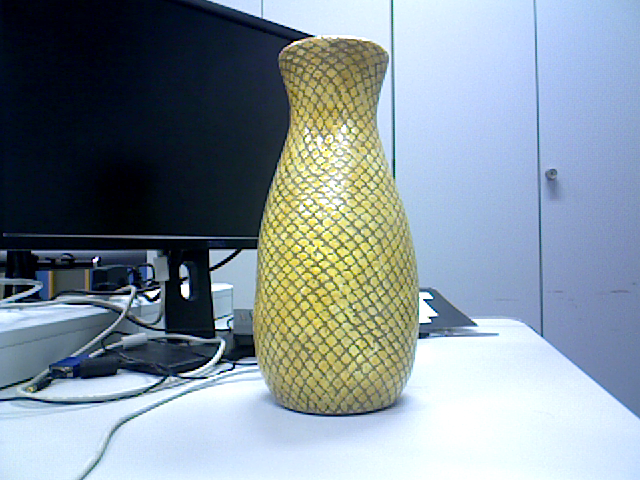
\includegraphics[width=0.45\textwidth]{figures/methodology/inpainting_rgb.png}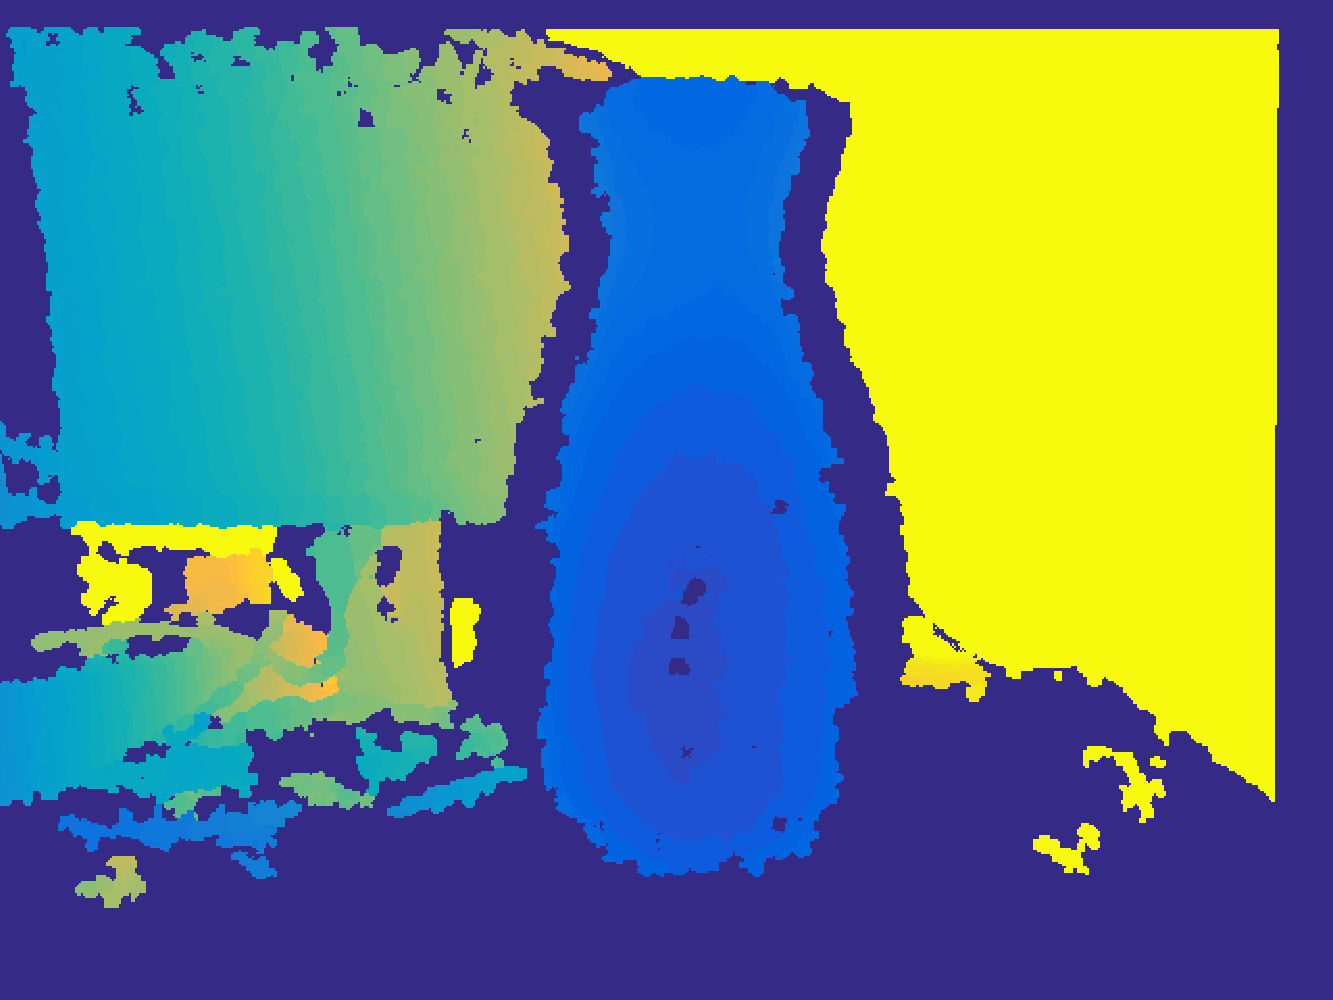
\includegraphics[width=0.45\textwidth]{figures/methodology/inpainting_depth.pdf}
% \caption{dd}
% \label{fig:inpainting1}
%\end{figure}

Image inpainting itself is a very mutual area and has been widely applied as a useful tool for many modern computer vision applications, e.g, restore the damaged parts of ancient paintings, or remove unwanted texts or objects in a photography~\cite{bertalmio2000image}. 
Since the idea of image inpainting is to automatically replace the lost or undesired parts of an image with the neighbouring information by interpolating, we were inspired to apply it to fill in the missing depth information (Fig.~\ref{fig:inpainting1}).

\begin{figure}[!htbp]
\centering
\subfigure[RGB image]{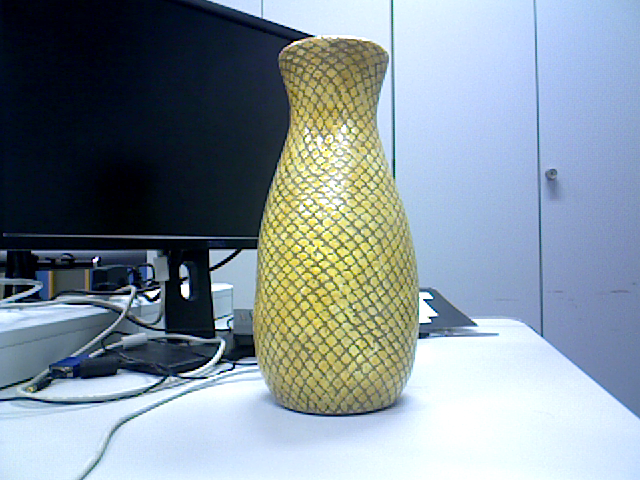
\includegraphics[width=0.45\linewidth]{figures/methodology/inpainting_rgb.png}}
\subfigure[Input depth image]{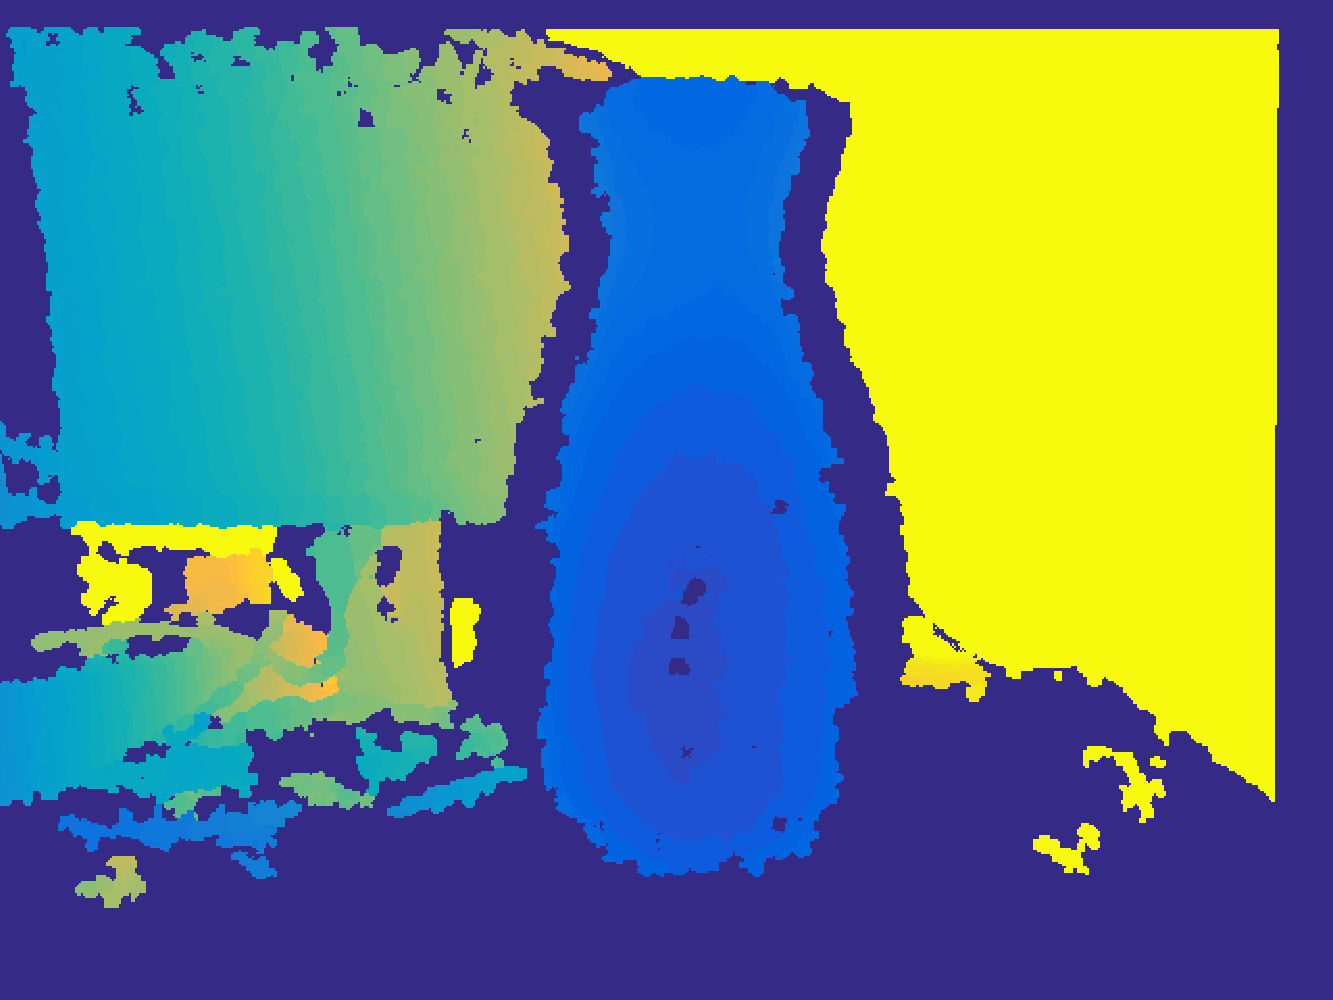
\includegraphics[width=0.45\linewidth]{figures/methodology/inpainting_depth.pdf}}
\caption{The input RGB and depth image of a vase. The depth map in (b) is visualized using color from blue (near) to yellow (far).}
\label{fig:inpainting1}
\end{figure}

It should be noted that, the depth inpainting is applied to the input noisy image so there is no need to use some powerful and advanced algorithms.
The only request is to fill the missing areas with inexpensive computational time.

The general mathematical form of a classic inpainting algorithm~\cite{bertalmio2000image} can be written as follows

\begin{equation}\label{eq:method_inpaint1}
I^{t+1}(i,j) = I^{t}(i,j) + \mu U^{t}(i,j), \forall(i,j)\in \Omega
\end{equation}
where $I(i,j)$ is the pixel value in image $I$, $t$ is the artificial time step, $\mu$ is the updating rate, $U$ is the update information and $\Omega$ are the area with missing information.

To build the update map $U$ in each time step, there are two principles that~\cite{bertalmio2000image} follow.
One is the inpainted values inside $\Omega$ should be as smooth as possible. 
The other is the lines reaching the edge of $\Omega$ should be continued and cross the missing area, while the values in $\Omega$ should be propagated from the nearest neighbours of $\Omega$ along the lines.

Again, due to the fact that our input depth images have poor quality, the lines arriving at the boundary $\delta \Omega$ may be incorrect or produced by the noises.
Thus, it is reasonable that our initial depth inpainting problem focuses on the smooth propagation from the neighbours and fill in the holes.

In each pixel $(x_0, y_0)$ inside $\Omega$, $U$ can be modelled as a discrete four-neighbour Laplacian operator:
\begin{equation}
\begin{split}
U(x_0, y_0) = \Delta I
		        = 4I(x_0, y_0) - I(x_0 + 1, y_0) - I(x_0 - 1, y_0) - I(x_0, y_0+1) - I(x_0 , y_0 -1)
\end{split}
\end{equation}
Now the inpainting problem in Eq.~\ref{eq:method_inpaint1} can be represented as a minimization problem: 
\begin{equation}
\min \iint\limits_{\Omega} |U(x,y)|^2 dxdy 
\end{equation}
This problem can be reformulated to a typical linear equation in matrix form:
\begin{equation}
\mathbf{Ax=b}
\end{equation}
Assuming $n$ is the number of pixel inside $\Omega$ and $m$ is the sum of $n$ and the number of neighbouring pixel around the boundary $\delta \Omega$, $\mathbf{A}$ is a $m\times n$ Laplacian matrix, $\mathbf{b}$ is a $m\times1$ vector containing all the known boundary depth values and the $0$ inside $\Omega$.
Solving the linear equation with simple least square method, we can acquire the inpainted values.
With our this naive image inpainting algorithm, we can fill the holes on the depth image as shown in Fig.~\ref{fig:pre-processing}.

%----------------------------------------------
\subsection{Depth denoising}
%----------------------------------------------
the depth images acquired from the RGB-D cameras with moderate price usually contain various noises. 
As a standard pre-processing method, the image denoising technique is also applied to our input inpainted depth map.
Similar to the state-of-the-art depth refinement methods~\cite{zhang2012edge, or2015rgbd, han2013high, or2016real, haque2014high, yu2013shading}, bilateral fitering~\cite{tomasi1998bilateral} is used as our depth pre-processing smoother. 

The advantages of bilateral filter is reducing the noise while preserving the edge in the input image. 
More than a regular Gaussian smooth filter, which uses only the difference of the image values (depth in our case) between the center pixel the neighbours, the bilateral filter also utilizes the space difference as a reference to build up the weighting function.
The filtered pixel value can be modelled as a weighted sum of neighbouring pixels:
\begin{equation}
\hat{I}(\mathbf{x}) = \frac{1}{W}\sum_{\mathbf{y} \in \mathcal{N}} I(\mathbf{y})e^{-(\frac{\lVert I(\mathbf{x}) - I(\mathbf{y})\rVert^2}{2\sigma_r^2} + \frac{\lVert \mathbf{x} - \mathbf{y}\rVert^2}{2\sigma_d^2})}
\end{equation}
where $\hat{I}(\mathbf{x})$ is the filtered value at pixel $\mathbf{x}$, $\mathcal{N}$ represents the neighbouring pixels with $\mathbf{x}$ in the center, and $W$ is the the sum of the all the weights. 
The smoothed result on our input depth image is shown in Fig.~\ref{fig:pre-processing}.

\begin{figure}[!htbp]
\centering
\subfigure[Input depth]{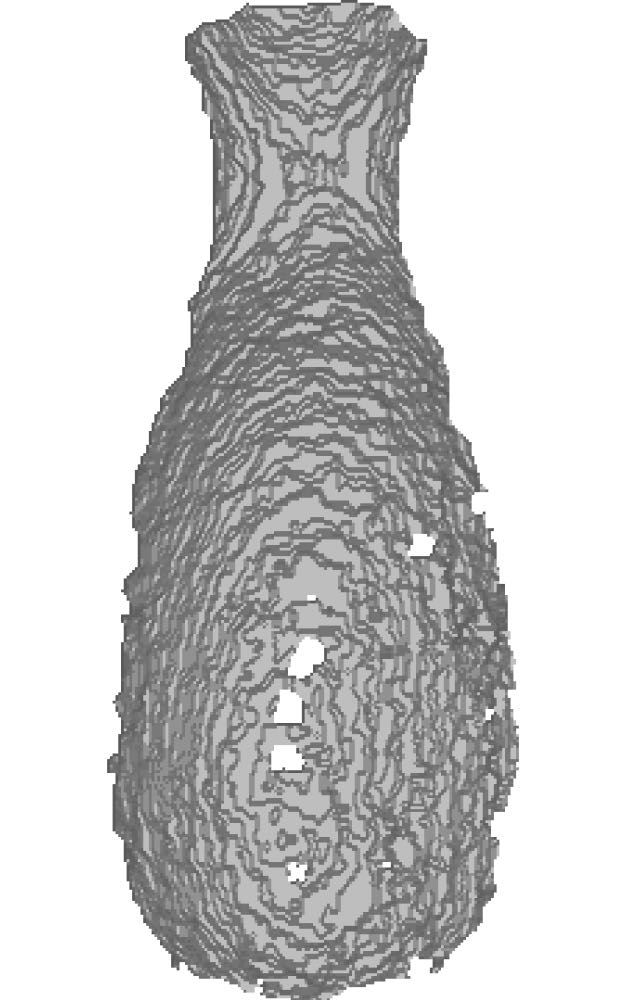
\includegraphics[width=0.30\linewidth]{figures/methodology/inpainting_shape_before.pdf}}
\subfigure[After inpainting]{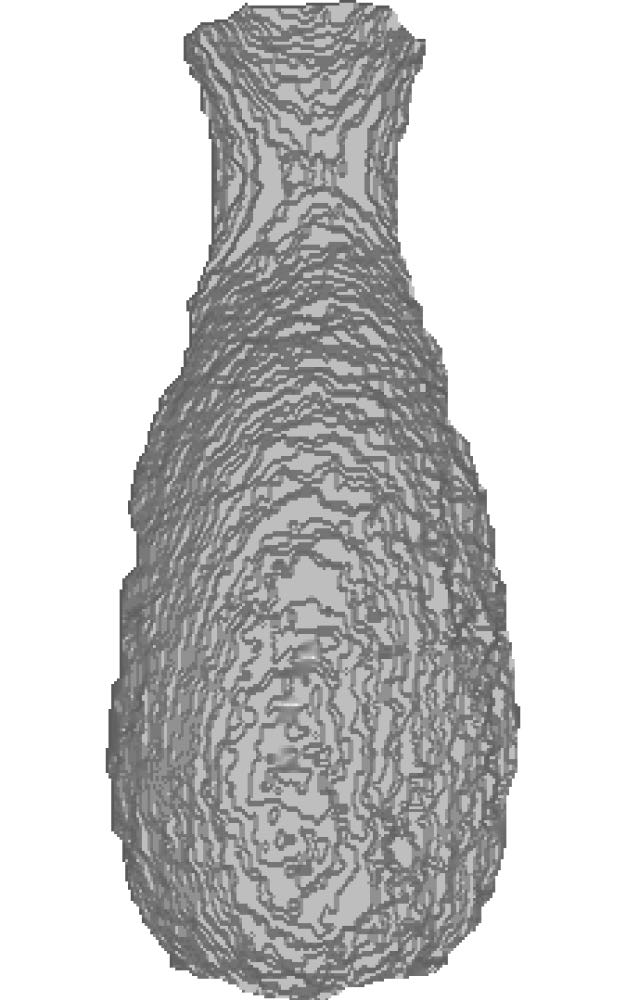
\includegraphics[width=0.30\linewidth]{figures/methodology/inpainting_shape_after.pdf}}
\subfigure[After smoothing]{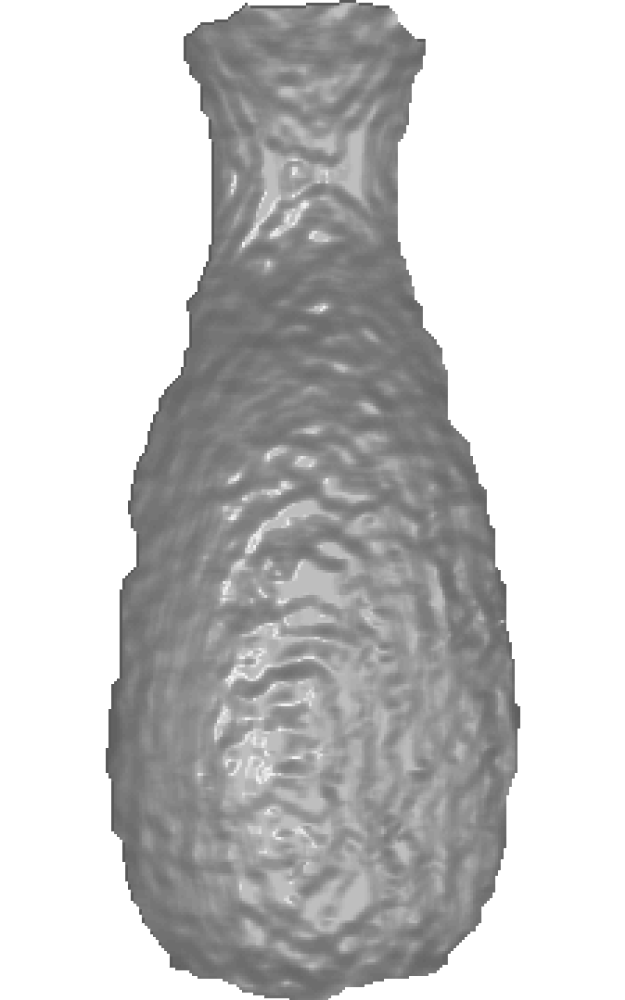
\includegraphics[width=0.30\linewidth]{figures/methodology/smooth_shape_after.pdf}}
\caption{Illustrations for the pre-processing on the depth of the vase.}
\label{fig:pre-processing}
\end{figure}

After the pre-processing procedure, we have an initial smooth and inpainted depth image. 
It will be used as the input of all the depth refinement methods detailed in the following sections.

%%%%%%%%%%%%%%%%%%%%%%%%%%%%%%%%%%%%%%%%%%%%
\section{RGBD-Fusion Like method}
%%%%%%%%%%%%%%%%%%%%%%%%%%%%%%%%%%%%%%%%%%%%
RGBD-Fusion is a state-of-the-art depth recovery method proposed by Or-El \emph{et al.}~\cite{or2015rgbd} in 2015.
This novel method is adequate for natural scene illumination and able to enhance the depth map much faster than other methods.
It is reasonable to gain a comprehensive understanding in the field of depth refinement by implementing this method with our own idea inside.

It is worth mentioning that we didn't just follow the paper step by step without injecting any our own ideas.
For example, instead of estimating the pixel-wise ambient light with a separate energy function, we jointly calculated all four first-order spherical harmonics parameters (3 for point-source light direction and 1 for ambient light) with a simple fast least square, and the results have only negligible difference.
And throughout the whole estimation process of light, albedo and depth, we only used the information within the given mask which also speeded up the algorithm.
This is the reason we call our first method "RGB-Fusion Like" method.

The natural uncalibrated illumination condition means the light is no longer a point light source, thus a Lambertian model is not sufficient. 
Basri and Jocobs~\cite{basri2003lambertian} has found that low order spherical harmonics (SH) model can well set out the irradiance of the diffused objects under the natural scene.
More specifically, the first-order SH model can capture 87.5\% of natural lighting, whose form is extended from the Lambertian model:
%$$$$$$$$$$$$$$$$$$
\begin{equation}\label{eq:rgbd_light_model}
I(x,y) = \rho(x,y)(\mathbf{l}^\top \mathbf{n}(x,y) + \varphi)
\end{equation}
%$$$$$$$$$$$$$$$$$$
where $I : \mathcal{M}\rightarrow \mathbb{R}^C$ is the irradiance of the objects, which is represented as the intensity values. 
$\rho : \mathcal{M}\rightarrow \mathbb{R}^C$ is the albedo, $\mathbf{l}^\top = \begin{pmatrix} l_x & l_y & l_z \end{pmatrix}$ describes the light direction and $\varphi$ represents the ambient light.
$\mathbf{n} : \mathcal{M}\rightarrow \mathbb{R}^3$ is the surface normal, which is dependent on the depth $z$.
We define that $C = 1$ represents the grayscale image while C = 3 for color image. 
$(x,y) \in \mathcal{M}$ represents the pixel coordinate inside the given mask $\mathcal{M}$ of an object.
Eq.~\ref{eq:rgbd_light_model} can be rewritten as:
%$$$$$$$$$$$$$$$$$$
\begin{equation}\label{eq:rgbd_light_model2}
I(x,y) = \rho(x,y) \; \mathbf{s}^\top \tilde{\mathbf{n}}(x,y)
\end{equation}
%$$$$$$$$$$$$$$$$$$
where
%$$$$$$$$$$$$$$$$$$
\begin{equation}
\mathbf{s} = \begin{pmatrix}\mathbf{l} \\ \varphi \end{pmatrix} 
 \; \; 
\tilde{\mathbf{n}}(x,y) = \begin{pmatrix}\mathbf{n}(x,y) \\ 1\end{pmatrix}
\end{equation}
%$$$$$$$$$$$$$$$$$$
$\mathbf{s}$ is the first-order SH parameters. It should be mentioned that the 1st-order SH model is used as the fundamental model throughout the whole methodology part.

After introducing the preliminary knowledge, the overall energy function for the RGBD-Fusion like method which can jointly estimate lights, albedo and depth is described below:
%$$$$$$$$$$$$$$$$$$
\begin{equation}\label{eq:rgbd_energy_rough}
    \begin{split}
        E(\rho, z, \mathbf{s}) = \; \mathop{\sum \sum}_{(x,y) \in \mathcal{M}} | I(x,y) - &\rho(x,y) \mathbf{s}^\top\tilde{\mathbf{n}}(x,y) |^2 
        + \lambda_{\rho} \mathop{\sum \sum}_{(x,y) \in \mathcal{M}} \sum_{k \in \mathcal{N}} |\omega_k(x,y) (\rho(x,y) - \rho_k) |^2 \\
        &+ \lambda_z \mathop{\sum \sum}_{(x,y) \in \mathcal{M}} | z(x,y) - z_0(x,y)|^2 + 
        \lambda_l \mathop{\sum \sum}_{(x,y) \in \mathcal{M}} |\Delta z(x,y) |^2
    \end{split} 
\end{equation}
%$$$$$$$$$$$$$$$$$$
For the sake of simplicity, we will use $\lVert \boldsymbol{\cdot} \rVert_2^2 =\mathop{\sum \sum}\limits_{(x,y) \in \mathcal{M}}(\cdot)^2$ to reshape the equation, and then $I$ and $\rho$ are vectorized to $\mathbb{R}^m$ within the mask, while $\tilde{\mathbf{n}} \in \mathbb{R}^{m\times 4} $. $m$ is the number of pixel inside the mask $\mathcal{M}$.
So Eq.~\ref{eq:rgbd_energy_rough} can be reformulated as:
%$$$$$$$$$$$$$$$$$$
\begin{equation}\label{eq:rgbd_energy}
	E(\rho, z, \mathbf{s}) = \; \lVert I - \rho \cdot \; \tilde{\mathbf{n}}(z)\mathbf{s} \rVert^2_2 + \lambda_{\rho} \lVert \sum_{k \in \mathcal{N}} \omega_k (\rho - \rho_k) \rVert^2_2 + \lambda_z \lVert z - z_0\rVert^2_2 + \lambda_l \lVert \Delta z \rVert^2_2
\end{equation}
%$$$$$$$$$$$$$$$$$$

The function consists of a SFS term, an albedo anisotropic Laplacian term, a depth data fidelity term and a depth isotropic Laplacian term. 
Now we will go into the details step by step.

%----------------------------------------------
\subsection{Light estimation}
%----------------------------------------------
Here the surface normal $\mathbf{n}$ is formulated with orthographic projection, i.e. 
\begin{equation}\label{eq:rgbd_normal}
	\mathbf{n}(x,y) = \frac{1}{\sqrt{1 + |\nabla z(x,y)|^2}}
	\begin{pmatrix} 
		 \nabla z(x,y)\\ 
		 -1
	 \end{pmatrix}
\end{equation}
$\nabla z(x,y)$ represents the gradient of depth image $z(x,y)$ in $x$ and $y$ directions.
Since we have the input depth from pre-processing, initial $\mathbf{n}_0$ is known.

In the sense of intrinsic image decomposition, an image can be decomposed as the product of albedo and shading, so we can treat $\mathbf{s}^\top \tilde{\mathbf{n}}(x,y) $ in Eq.~\ref{eq:rgbd_light_model2} as the shading.

To compute the spherical harmonics parameters, we assume the albedo $\rho$ equals to $1$ for each pixel. 
Since there are known intensity value and surface normal in each pixel within the mask, we will have an overdetermined least square problem from the energy in Eq.~\ref{eq:rgbd_energy}: 
\begin{equation}\label{eq:rgbd_light_estimate}
\min_{\mathbf{s}} \; \lVert \tilde{\mathbf{n}} \mathbf{s} - I \rVert^2_2
\end{equation}
This process only need to be applied once at the beginning of the process since the least squares is not sensitive to the details on the surface, thus the estimation from the smooth surface is enough.

%----------------------------------------------
\subsection{Albedo estimation}\label{sec:rgbd_albedo_estimation}
%----------------------------------------------
As mentioned in Chapter~\ref{chap:background}, many depth recovery methods based on SFS or photometric stereo techniques assume constant or uniform albedo.
Such assumption does not fit in with the real-world objects, and hence, they perform poorly on the shape estimation for multi-albedo cases.
In order to acquire a satisfying shape outcome, an effective multi-albedo estimation process is a matter of importance.

We know from Eq.~\ref{eq:rgbd_light_model} that, assuming we have the knowledge of input intensity and estimated shading, the albedo image can be directly obtained from $I/S$.
However, such albedo is prone to the overfitting, which make the acquired albedo contain all the undesired spatial layout details.
This is due to the fact that both input image $I$ and the surface normal $\mathbf{n}$ are noisy.
To resolve the overfitting problem, we should impose some restrictions on the estimation of albedo.
A large amount of our daily objects have piecewise smooth appearance, which means most pieces of a layout are dominated by certain colors.
Therefore, a prior that emphasizes the piecewise smoothness on the albedo should be defined.

The albedo of an object can be roughly divided to several pieces with different intensities, which can be treated as the image segmentation problem to some extend. 
Thus, we should refer to some classic variational segmentation methods and adapt the edge preserving smoothness term to our problem.
Similar to the idea in~\cite{casaca2014laplacian}, an anisotropic Laplacian term is imposed to estimate the albedo.
Now, the SH parameters $\mathbf{s}$ and the surface normal $\mathbf{n}$ are fixed, the overall regularized minimization problem in Eq.~\ref{eq:rgbd_energy} is:

\begin{equation}\label{eq:rgbd_albedo_estimate}
	\min_{\rho} \; \lVert \rho \cdot \tilde{\mathbf{n}} \mathbf{s} - I\rVert^2_2 + \lambda_{\rho} \lVert \sum_{k \in \mathcal{N}} \omega_k (\rho - \rho_k) \rVert^2_2
\end{equation}
where $k$ indicates the neighbouring index of a certain pixel, which 4-connected set is chosen for $\mathcal{N}$ in our case. 
The weight $\omega_k$ is defined as below, and it is dependent to two parameters $\sigma_I$ and $\sigma_z$ which accounts for the discontinuity in both intensity and depth.
\begin{equation}
	\omega_k=\exp\Bigg(-\dfrac{\lVert I - I_k \rVert^2_2}{2\sigma_I^2} -\dfrac{\lVert z - z_k \rVert^2_2}{2\sigma_z^2}\Bigg)
\end{equation}

%----------------------------------------------
\subsection{Depth enhancement}
%----------------------------------------------
After acquiring the first-order spherical lighting parameters $\mathbf{s}$ and the albedo $\rho$, we can refine our depth with the help of Eq.~\ref{eq:rgbd_light_model} and Eq.~\ref{eq:rgbd_normal}.
Now our minimization problem with respect to the depth $z$ in Eq.~\ref{eq:rgbd_energy} can be written as below. 
The data fidelity term is applied to resolve the SFS ambiguities and enables our refined surface close to the input. The Laplacian smoothness term makes sure that there is no strong discontinuity in the output. 
\begin{equation}\label{eq:rgbd_depth_refine}
	\min_{z} \; \lVert \rho \cdot \tilde{\mathbf{n}}(z) \mathbf{s} - I \rVert^2_2 + \lambda_z \lVert z - z_0\rVert^2_2 + \lambda_l \lVert \Delta z \rVert^2_2
\end{equation}
where $z_0$ is the input depth and $\Delta$ represents the  Laplacian operator. 
It can be easily noticed that this introduced function is non-linear because the normal in our SFS term contains a denominator related to the depth gradient. 
Many optimization methods can be applied to solve the non-linear problem, e.g. Levenberg-Marquardt algorithm or ADMM, but they are not suitable in our application due to expensive computational time. 
Here a "fixed point" method which is similar to iteratively reweighted least square (IRLS) has been introduced to deal with our problem efficiently. 

The idea of the fixed-point approach is in each iteration, the normalizer in the surface normal can be treated as a weighting term and determined by the depth from last iteration.
With the help of this trick, the normalizer is known and Eq.~\ref{eq:rgbd_depth_refine} is linear again.
We can solve the linear system using any fast linear optimization method.
In each iteration $t$, this process can be represented element-wise as follows:
\begin{equation}
	\begin{split}
		\mathbf{n}^{(t)}(z^{(t)}, z^{(t-1)}) &= w(z^{(t-1)})
		\begin{pmatrix} 
			 \nabla z^{(t)}\\ 
			 -1
	         \end{pmatrix}\\
	         w(z^{(t-1)}) &=  \frac{1}{\sqrt{1 + |\nabla z^{(t-1)}|^2}}
	\end{split}
\end{equation}
And now the depth refinement problem in Eq.~\ref{eq:rgbd_depth_refine} is reformulated as below in each iteration:

\begin{equation}\label{eq:rgbd_depth_refine2}
	\min_{z^{(t)}} \; \lVert \rho \cdot \tilde{\mathbf{n}}(z^{(t)}, z^{(t-1)}) \mathbf{s} -I\rVert^2_2 + \lambda_z \lVert z^{(t)} - z_0\rVert^2_2 + \lambda_l \lVert \Delta z^{(t)} \rVert^2_2
\end{equation}
As long as the energy decreases in each iteration, the process is repeated.

To sum up the approach in this section, it should be noted that the SFS term in the overall energy (Eq.~\ref{eq:rgbd_energy} was used as a core in all light, albedo and depth estimation.
The whole process of RGBD-Like method has been described in Alg.~\ref{alg:rgbd_fusion}. 



\begin{algorithm}[!htbp]
	\begin{algorithmic}[1]
  		\caption{\textbf{RGBD-Fusion Like Depth Refinement}}
		\label{alg:rgbd_fusion}
		 \renewcommand{\algorithmicrequire}{\textbf{Input:}}
		 \renewcommand{\algorithmicensure}{\textbf{Output:}}
		 \REQUIRE Initial depth image $z_0$, RGB image $I$
		 \vspace{1.8mm}
		 \STATE Estimate SH parameter, $\mathbf{s} = \argmin \limits_{\mathbf{s}} \; E(\rho = 1, z_0)$ \COMMENT{Eq.~\ref{eq:rgbd_light_estimate}}
		 \STATE Estimate albedo, $\rho = \argmin \limits_{\rho} \; E(z_0, \mathbf{s})$ \COMMENT{Eq.~\ref{eq:rgbd_albedo_estimate}}
		 \STATE t = 1, $z^{(t-1)} = z_0$
		 \vspace{1.8mm}
		  \WHILE {$ E(\rho, z^{(t)}, \mathbf{s}) - E(\rho, z^{(t-1)}, \mathbf{s}) < 0$}
		   \vspace{1.8mm}
			  \STATE $z^{(t)} = \argmin \limits_{z} E(\rho, z, \mathbf{s})$ \COMMENT{Eq.~\ref{eq:rgbd_depth_refine2}}
		          \STATE $t := t + 1$
		 \vspace{1.8mm}
		  \ENDWHILE
		  \ENSURE  Refined depth image $z^{(t)}$
	\end{algorithmic}
\end{algorithm}


%----------------------------------------------
\subsection{Limitations}
%----------------------------------------------

Although our RGBD-Fusion like method works moderately well in many real cases, it is not difficult to find the limitations and improve correspondingly.
\begin{itemize}
\item the surface normal modelled by the orthographic projection is merely an ideal case, but it is not really in line with the real world camera model.
And the intrinsic parameters such as the focal length and the coordinate of the principle point are either usually given as a preliminary knowledge, or obtained from calibration without much effort.
Hence, it is reasonable to formulate the surface normal with the perspective projection model.

\item In our RGBD-Fusion like method, only the intensity is applied because the values in RGB channels are more or less the same under the natural scene illumination. 
When we estimated the SH lighting parameters and the albedo in 3 channels separately, the results are quite similar to each other.
So using all three channel rather than just the intensity value will not provide much extra information and improve the depth enhancement. 
Instead, it will just decelerate the whole algorithm.
We ought to find a way to take better advantages of all three channels.

\item The most important inspiration for us to propose RGB ratio model in the next section is, the RGBD-Fusion like method was not convergent in terms of depth enhancement part because of the fix-point method.
In the $4$th line of the Alg.~\ref{alg:rgbd_fusion}, we make the iteration stop when the energy for the depth refinement starts increasing.
This is due to the reason that the fixed-point method actually tries to solve the non-linearity in a tricky way, which is mathematically not totally correct. 
Therefore, we thought of the idea of RGB ratio model, which can eliminate the denominator inside the normal and promise a real linear problem.

\end{itemize}


%%%%%%%%%%%%%%%%%%%%%%%%%%%%%%%%%%%%%%%%%%%%
\section{Proposed method I: RGB Ratio Model}
%%%%%%%%%%%%%%%%%%%%%%%%%%%%%%%%%%%%%%%%%%%%

According to the limitations in the last section, we thought of the idea of RGB ratio model.
First of all, we replace the orthographic projection model with the perspective one.
And then, to fully use the information of the RGB three channels while eliminating the non-linearity in the objective function in the depth refinement, we use the ratio model between every two channels among the three.

It should be noted that we need to add active R, G and B 3 LED lights for the sake of emphasizing the difference among RGB channels.
The green LED is installed in the middle with the red and blue ones on the two sides of ASUS Xtion Pro Live camera (both are around 30 cm to the green LED).
The hardware setup and a color image taken with such setup are illustrated in Fig.~\ref{fig:ratio_setup}.

\begin{figure}[!htbp]
\centering
\subfigure[LED lights setup]{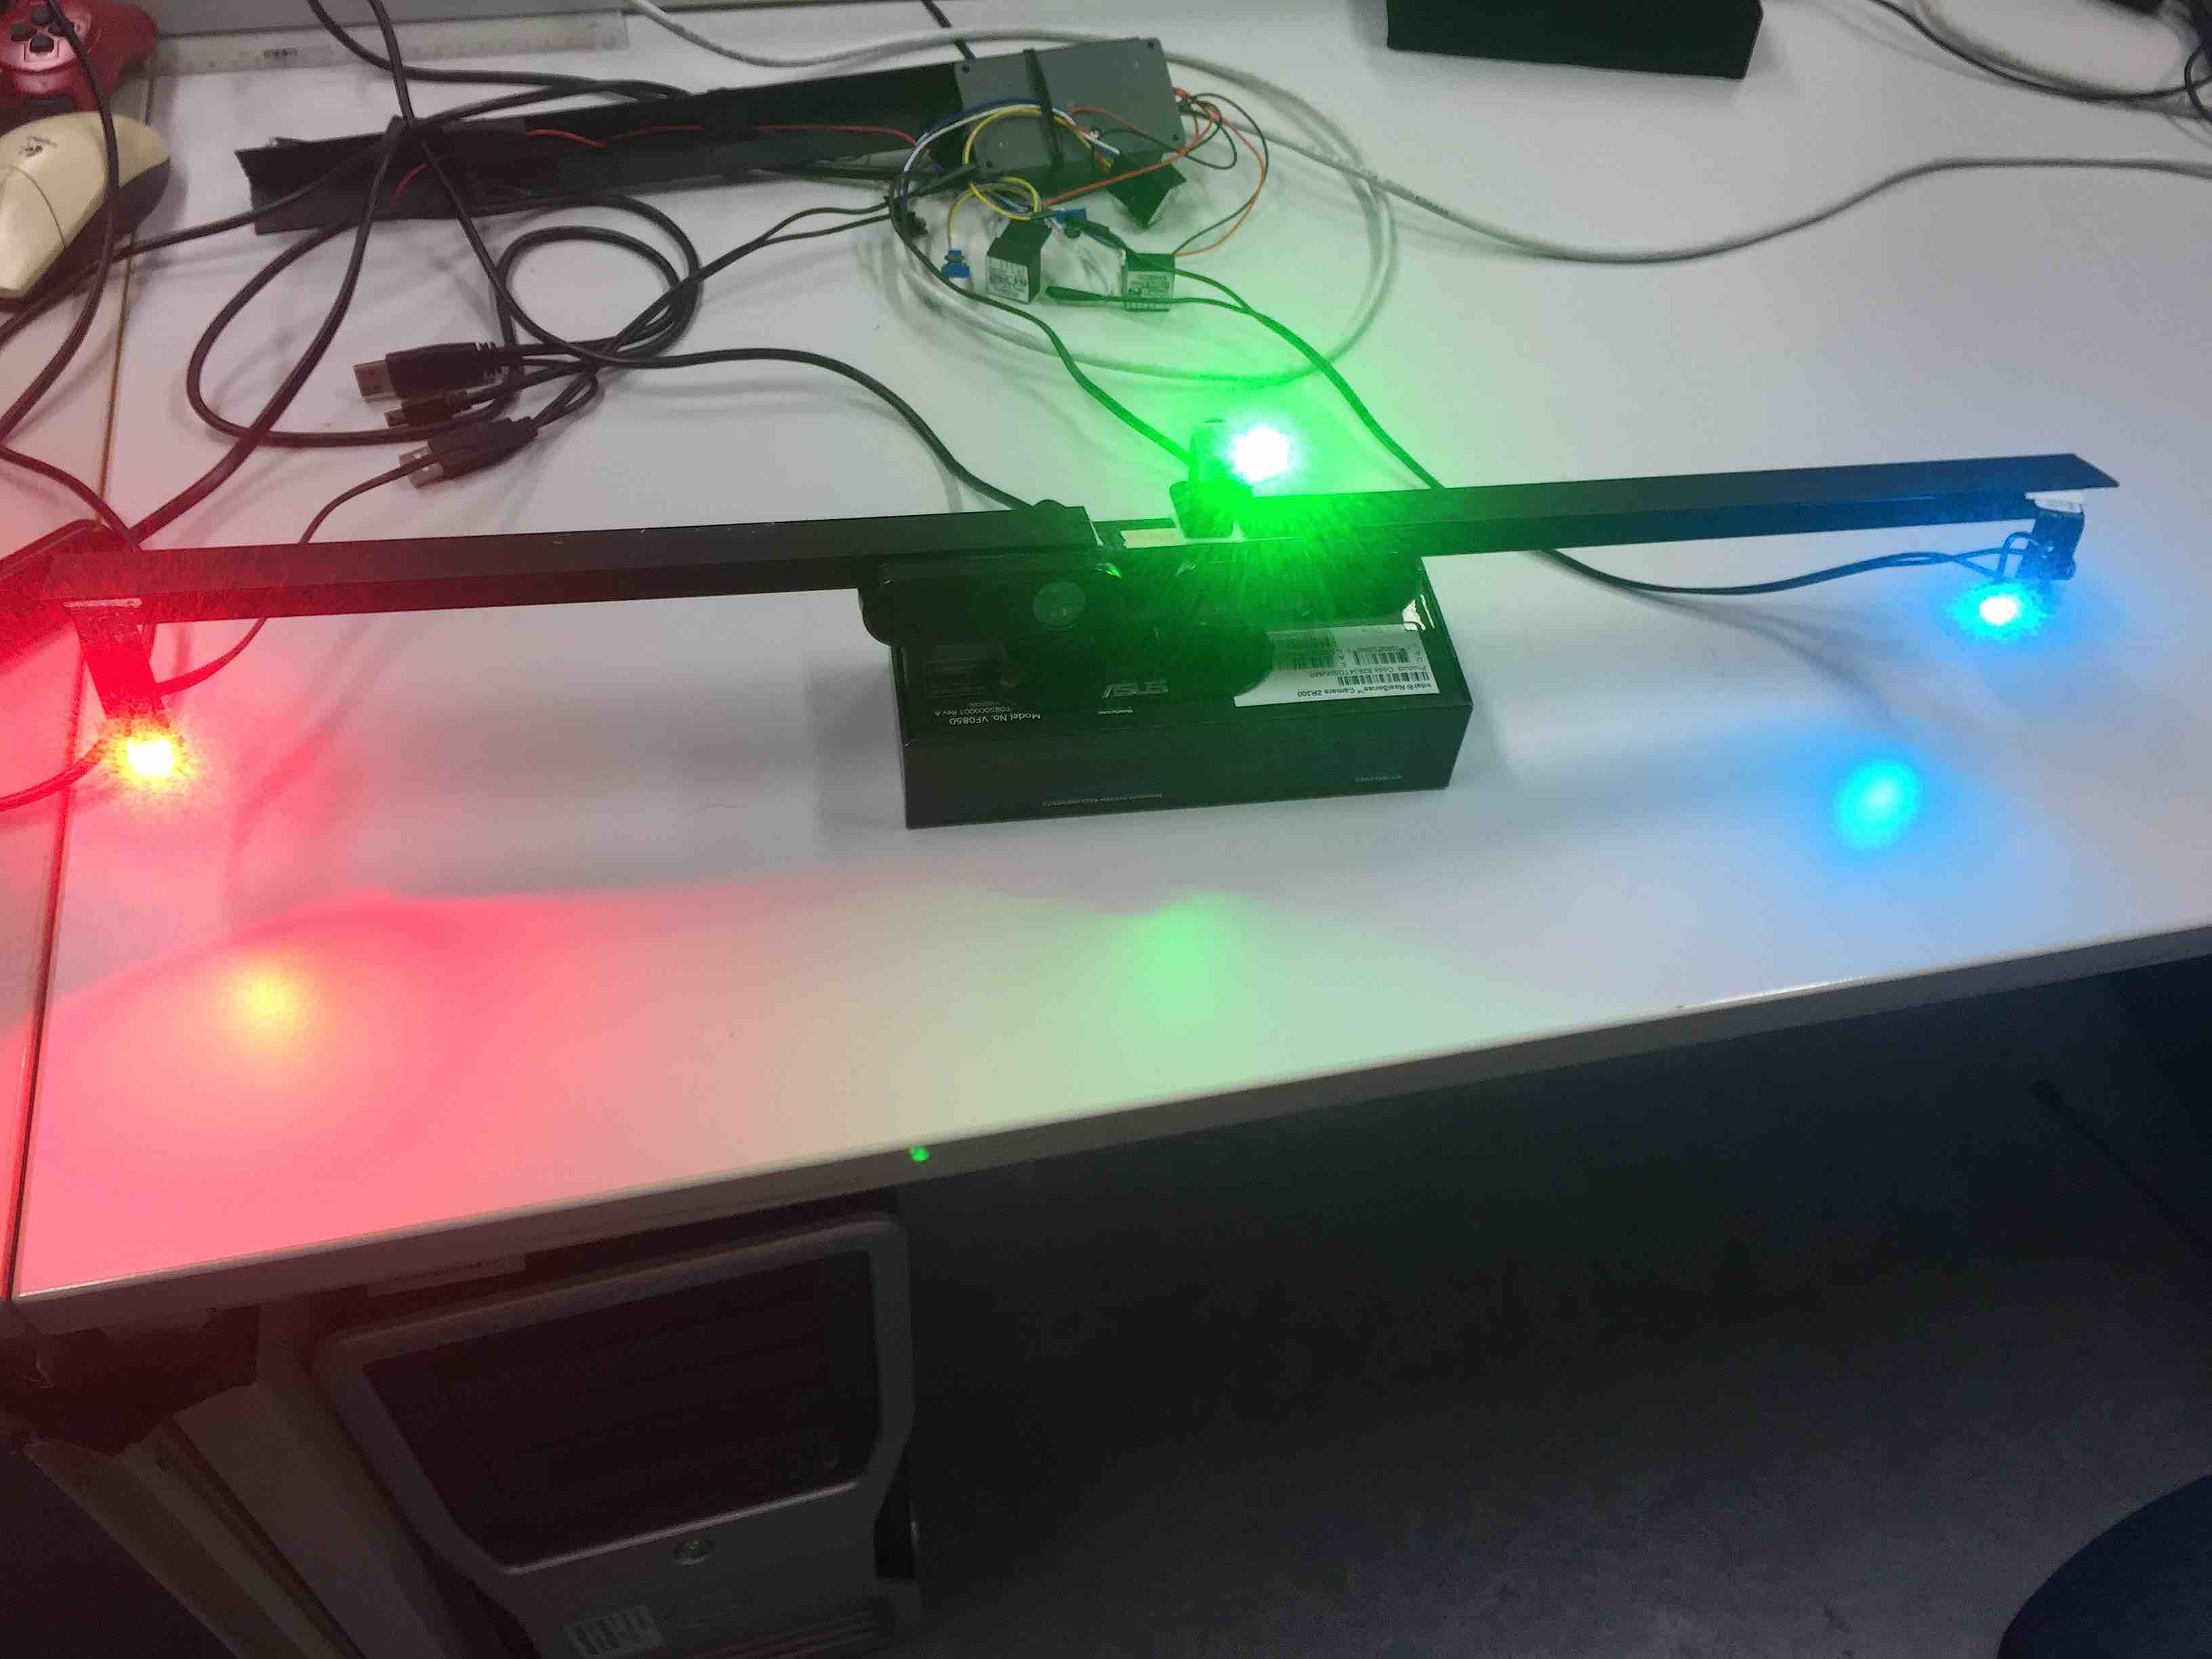
\includegraphics[width=0.45\linewidth]{figures/methodology/ratio_setup.JPG}}
\subfigure[A color image with our lighting setup]{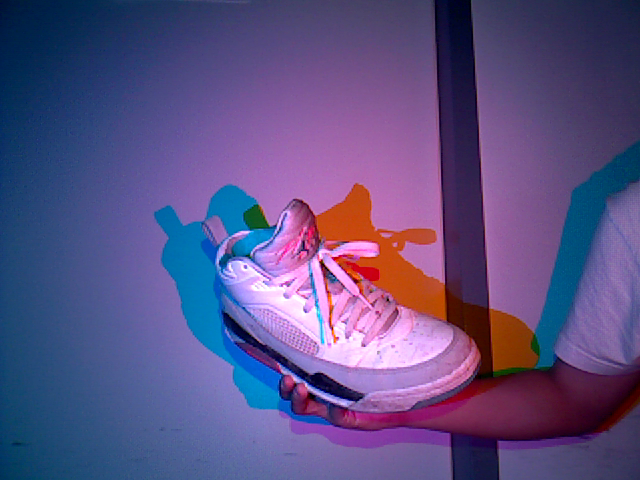
\includegraphics[width=0.45\linewidth]{figures/methodology/ratio_setup_view.png}}
\caption{Illustrations for the RGB LED setup and the corresponding image.}
\label{fig:ratio_setup}
\end{figure}


Now to derive our new ratio model, we treat each channel of the color image $I$ as an single intensity image, denoted by $I_R, I_G, I_B$.
Therefore, 3 equations can be obtained from Eq.~\ref{eq:rgbd_light_model}.

\begin{equation}\label{eq:ratio_prepare}
    \begin{split}
	I_R &= \rho_R(\mathbf{l}_R^\top \mathbf{n} + \varphi_R)\\
	I_G &= \rho_G(\mathbf{l}_G^\top \mathbf{n} + \varphi_G)\\
	I_B &= \rho_B(\mathbf{l}_B^\top \mathbf{n} + \varphi_B)
    \end{split}
\end{equation}

Using R and G channel as an example, we acquire the ratio model:

\begin{equation}\label{eq:ratio_rg_sh1}
%\begin{split}
\frac{I_R - \rho_R \varphi_R}{I_G - \rho_G \varphi_G} = \frac{\rho_R \mathbf{l}_R^\top \mathbf{n}}{\rho_G \mathbf{l}_G^\top \mathbf{n}}
%\rho_G (I_R - \rho_R \varphi_R)\mathbf{l}_G^T \mathbf{n} & = \rho_R (I_G - \rho_G \varphi_G)\mathbf{l}_R^T\mathbf{n}\\
%\end{split}
\end{equation}

Similarly, we can acquire another two ratio models which are between green and blue, and blue and red channels respectively.
We are able to notice from Eq~\ref{eq:ratio_rg_sh1} that, the non-linearity problem mentioned before has been solved because the denominator in the surface normal $\mathbf{n}$ is cancelled out.
Also, our normal is derived from perspective camera model and can be represented as a function of $\; \log z$. 
For the sake of simplicity we directly represent $z = \log z$ and redefine $\mathbf{n}$ without the normalizer in the following part.
%$$$$$$$$$$$$$$$$
\begin{equation}\label{eq:ratio_normal}
    \mathbf{n}(x,y) =
     \begin{pmatrix}
         fz_x(x,y)\\
         fz_y(x,y)\\
         -1 - \tilde{x}z_x(x,y) - \tilde{y}z_y(x,y)
     \end{pmatrix}
\end{equation}
%$$$$$$$$$$$$$$$$
where $f$ is the focal length, $(\tilde{x}, \tilde{y}) = (x- x_0, y - y_0)$, with $(x_0, y_0)$ the coordinates of principle points and $(x,y)$ the coordinate of a pixel inside the given mask, $[z_x, z_y]$ is the gradient of depth $z$.

The overall energy for the proposed RGB ratio model method is:
\begin{equation}\label{eq:ratio_energy}
    \begin{split}
	E(\mathcal{P}^{(t)}, z^{(t)}, \mathbf{s}^{(t)}) = \; &\lVert Ratio(\mathcal{P}^{(t)}, z^{(t)}) \rVert^2_2 
	+ \lambda_z||z^{(t)} - z_0||^2 \\&
	+ \lambda_{\rho}^1 \lVert \omega \nabla \mathcal{P}^{(t)} \rVert^2  
	+ \lambda_{\rho}^2 \lVert \mathcal{P} - \mathcal{P}^{(t-1)}\rVert^2 
	+ \sum_{c} \lVert \rho_c \; \mathbf{s}_c^\top \tilde{\mathbf{n}} - I_c \rVert^2_2, \; c\in\{R,G,B\}
    \end{split}
\end{equation}
where $\mathcal{P}$ is the stack of RGB albedo.
This energy is composed of a proposed ratio SFS term, a depth fidelity term, an albedo smoothness term, an albedo fidelity term and a SH estimation term.
Now we will explain our proposed algorithm based on the new ratio model.

%The key to this ratio model is toenlarge the difference of pixel values, light directions and the albedo in 3 channels

%----------------------------------------------
\subsection{Algorithm details}
%----------------------------------------------
Similar to the RGBD-Fusion Like method, the algorithm is separated to 3 parts: light estimation, albedo estimation and depth enhancement.
However, our new method requires an initial estimation of the color albedo as the input of our iterative method, and hence, we calculate the initial SH parameters $\mathbf{l}^{0}$ with Eq.~\ref{eq:rgbd_light_model} and the color albedo $\mathcal{P}^{0}$ with Eq.~\ref{eq:rgbd_albedo_estimate} using the old model.
Noted that the initial estimation is performed with respect to all RGB three channels.

\textbf{Albedo refinement:}
with the acquired $\rho^{0}$ and $\mathbf{l}^{0}$, we can start the iteratively refinement process.
In order to refine the color albedo with our ratio model, in each iteration, we need to reshape the ratio model described in Eq.~\ref{eq:ratio_rg_sh1} as follows:
\begin{equation}\label{eq:ratio_albedo_prepare}
\begin{split}
I_G \mathbf{l}_R^\top\mathbf{n} \rho_R - I_R \mathbf{l}_G^\top\mathbf{n} \rho_G  = \rho_R \rho_G (\varphi_G\mathbf{l}_R^\top \mathbf{n} - \varphi_R\mathbf{l}_G^\top \mathbf{n})\\
I_B \mathbf{l}_G^\top\mathbf{n} \rho_G - I_G \mathbf{l}_B^\top\mathbf{n} \rho_B  = \rho_G \rho_B (\varphi_B\mathbf{l}_G^\top \mathbf{n} - \varphi_G\mathbf{l}_B^\top \mathbf{n})\\
I_R \mathbf{l}_B^\top\mathbf{n} \rho_B - I_B \mathbf{l}_R^\top\mathbf{n} \rho_R  = \rho_B \rho_R (\varphi_R\mathbf{l}_B^\top \mathbf{n} - \varphi_B\mathbf{l}_R^\top \mathbf{n})
\end{split}
\end{equation}
For each pixel, we can reformulate the Eq.~\ref{eq:ratio_albedo_prepare} to a matrix form:
%$$$$$$$$$$$$$$$$
\begin{equation}\label{eq:rho_matrix}
    \begin{pmatrix}
        I_G \mathbf{l}_R^\top\mathbf{n} & - I_R \mathbf{l}_G^\top\mathbf{n} & 0 \\
        0 & I_B \mathbf{l}_G^\top\mathbf{n} & - I_G \mathbf{l}_B^\top\mathbf{n} \\
        - I_B \mathbf{l}_R^\top\mathbf{n} & 0 & I_R \mathbf{l}_B^\top\mathbf{n} 
    \end{pmatrix}
    \begin{pmatrix}
        \rho_R(x,y)\\
        \rho_G(x,y)\\
        \rho_B(x,y)
     \end{pmatrix}_{3 \times 1}
    =
    \begin{pmatrix}
        \rho_R \rho_G (\varphi_G\mathbf{l}_R^\top \mathbf{n} - \varphi_R\mathbf{l}_G^\top \mathbf{n})\\
        \rho_G \rho_B (\varphi_B\mathbf{l}_G^\top \mathbf{n} - \varphi_G\mathbf{l}_B^\top \mathbf{n})\\
        \rho_B \rho_R (\varphi_R\mathbf{l}_B^\top \mathbf{n} - \varphi_B\mathbf{l}_R^\top \mathbf{n})
    \end{pmatrix}
\end{equation}
This small linear system can be generalized to a big sparse linear system denoted as $\mathbf{A}_{\rho}\cdot {\mathcal{P}} = \mathbf{b}_{\rho}$.
The structure of this equation can be found in Appendix~\ref{appendix:implement}.
Here, $\mathcal{P}$ represents the stack of RGB three albedos.
%$$$$$$$$$$$$$$$$

To acquire the RGB albedos, some regularization terms are required similar to Eq.~\ref{eq:rgbd_albedo_estimate}. Now in each iteration, we fix the normal and the SH parameters, the minimization problem of color albedo in Eq.~\ref{eq:ratio_energy} in each iteration now becomes:
%$$$$$$$$$$$$$$$$
\begin{equation}\label{eq:ratio_albedo_refine}
    \mathcal{P}^{(t)} = 
    \argmin_{\mathcal{P}} \lVert\mathbf{A}_{\rho}^{(t-1)}\mathcal{P} - \mathbf{b}_{\rho}^{(t-1)}\rVert^2 
    + \lambda_{\rho}^1 \lVert \omega \nabla \mathcal{P} \rVert^2  
    + \lambda_{\rho}^2 \lVert \mathcal{P} - \mathcal{P}^{(t-1)}\rVert^2
\end{equation}
where the weight $\omega = \begin{pmatrix} \omega_R\\ \omega_G\\ \omega_B \end{pmatrix}$, which can be denoted as:
\begin{equation}
\omega_c = \exp(- \frac{\sigma_c ||\nabla I_c||^2}{\max ||\nabla I_c||^2}), \quad c \in \{R,G,B\}
\end{equation}
$\sigma_c$ is a tuning parameter for each channel $c$.  

%$$$$$$$$$$$$$$$$
There are three interesting aspects about the albedo estimation which worth having a few more words:
\begin{enumerate}
    \item One observation about Eq.~\ref{eq:rho_matrix} is that, if the SH parameters are the same among the three channels, the right side of the equal sign is or close to 0. 
    This is the reason why we need to set up 3 LED lights with a distance to each other, which will provide us enough difference on the light directions.
    \item Instead of using anisotropic Laplacian regularization in RGBD-Like method, the smoothness term in Eq.~\ref{eq:ratio_albedo_refine} only takes the use of the gradient of $\rho$ with a weight only depending on the RGB image's gradient.
    It takes less efforts to build such a smoothness term than the anisotropic term, but the acquired albedo is still satisfying.
    \item If we don't use a data fidelity term $\lVert \mathcal{P} - \mathcal{P}^{(t-1)}\rVert^2$, the albedo will get increasingly dark after several iterations. 
    This is due to the fact that there also exist the RGB albedos in $\mathbf{b}_{\rho}$, so $\rho = 0$ will become the solution of our ratio model term.
    Therefore, adding the data term can not only avoid such problem, but help refine the albedo iteratively. 
\end{enumerate}

{\color{red} need to add the albedo estimation 1, ground truth, 2, without regularization, 3, without weighting, 4 with weighting}

\textbf{Depth refinement}:
After acquiring the color albedo in time step $t$, we are going to refine the depth with the help of the ratio model.
First we reshape Eq.~\ref{eq:ratio_rg_sh1} with the surface normal $\mathbf{n}$ as the argument:
%$$$$$$$$$$$$$$$$
\begin{equation}\label{eq:ratio_depth1}
\begin{split}
\rho_G (I_R - \rho_R \varphi_R)\mathbf{l}_G^T \mathbf{n} - \rho_R (I_G - \rho_G \varphi_G)\mathbf{l}_R^T\mathbf{n} = 0\\
\rho_B (I_G - \rho_G \varphi_G)\mathbf{l}_B^T \mathbf{n} - \rho_G (I_B - \rho_B \varphi_B)\mathbf{l}_G^T\mathbf{n} = 0\\
\rho_R (I_B - \rho_B \varphi_B)\mathbf{l}_R^T \mathbf{n} - \rho_B (I_R - \rho_R \varphi_R)\mathbf{l}_B^T\mathbf{n} = 0 
\end{split}
\end{equation}
since the normal $\mathbf{n}$ now is a function of $z$, Eq.~\ref{eq:ratio_depth1} can be actually simplified as below (the derivation details can be found in Appendix~\ref{appendix:implement}):
\begin{equation}
    \Psi z = 0
\end{equation}
When the estimated color albedo and light are fixed, the depth refinement problem in Eq.~\ref{eq:ratio_energy} is:

\begin{equation}\label{eq:ratio_depth_refine}
    z^{(t)}= \argmin_{z}  ||\Psi z||^2 + \lambda_z||z - z_0||^2
\end{equation}

\textbf{Light estimation}
Since estimating light with the proposed ratio model is a ill-posed problem, we decided to use Eq.~\ref{eq:rgbd_light_estimate} to calculate the SH parameters for each channel when the albedo and the surface normal are freezed. The minimization problem from Eq.~\ref{eq:ratio_energy} can then be written as:
\begin{equation}\label{eq:ratio_light_estimate}
    \mathbf{s}^{(t)} = \argmin_{\mathbf{s} = (\mathbf{s}_R, \mathbf{s}_G, \mathbf{s}_B)}\sum_{c} \lVert \rho_c \; \mathbf{s}_c^\top \tilde{\mathbf{n}} - I_c\rVert^2_2, \; c\in\{R,G,B\}
\end{equation}

\begin{algorithm}[!htbp]
	\begin{algorithmic}[1]
  		\caption{\textbf{RGB Ratio Model method}}
		\label{alg:rgb_ratio}
		 \renewcommand{\algorithmicrequire}{\textbf{Input:}}
		 \renewcommand{\algorithmicensure}{\textbf{Output:}}
		 \REQUIRE Initial depth image $z_0$, RGB image $I$, mask, focal length, principle point
		 \vspace{1.8mm}
		 \STATE $\mathbf{s}^{(0)} = \argmin \limits_{\mathbf{s}} E(\mathcal{P} =1, z_0)$ \COMMENT{Eq.~\ref{eq:ratio_light_estimate}}
		 \STATE Estimate initial color albedo and build $\mathcal{P}^{(0)}$  \COMMENT{Eq.~\ref{eq:rgbd_albedo_estimate}}
		 \STATE t = 1, $z^{(0)} = z_0$
		 \vspace{1.8mm}
		  \WHILE {$ \frac{\Vert E(\mathcal{P}^{(t)}, z^{(t)}, \mathbf{s}^{(t)}) - E(\mathcal{P}^{(t-1)}, z^{(t-1)}, \mathbf{s}^{(t-1)})\Vert}{E(\mathcal{P}^{(t-1)}, z^{(t-1)}, \mathbf{s}^{(t-1)})} > \epsilon$}
		   \vspace{1.8mm}
			\STATE $\mathcal{P}^{(t)} = \argmin \limits_{\mathcal{P}} E(\mathcal{P}^{(t-1)}, z^{(t-1)}, \mathbf{s}^{(t-1)})$ \COMMENT{Eq.~\ref{eq:ratio_albedo_refine}}
			  \STATE $z^{(t)} = \argmin \limits_{z} E(\mathcal{P}^{(t)}, \mathbf{s}^{(t-1)})$ \COMMENT{Eq.~\ref{eq:ratio_depth_refine}}
			  \STATE $\mathbf{s}^{(t)} = \argmin \limits_{\mathbf{s}} E(\mathcal{P}^{(t)}, z^{(t)})$ \COMMENT{Eq.~\ref{eq:ratio_light_estimate}}
			  \vspace{1.8mm}
		          \STATE $t := t + 1$
		 \vspace{1.8mm}
		  \ENDWHILE
		  \ENSURE  Refined depth image $z^{(t)}$ and stacked color albedo $\mathcal{P}^{(t)}$
	\end{algorithmic}
\end{algorithm}

%----------------------------------------------
\subsection{Limitations}
%----------------------------------------------
Our method can estimate the albedo and the depth better than our RGBD-Fusion like method in some cases because the non-linearity optimization problem for the RGBD-Fusion like method has been solved.
Still, there exist some defects for our new RGB ratio model.
\begin{itemize}
\item Three LED lights have to be set up far away from each other.
	As already mentioned about Eq.~\ref{eq:ratio_albedo_prepare} , the albedo refinement may fail if the lights are too close and thus, we need to put 3 lights too near. 
	This can lead to some inconvenience, such as the requirement of enough space to put the system.
\item RGB three lights is likely to bring extra specularity.
	 If we want to refine the depth of an specular objects, the specular reflection will be from not only the natural scene illumination, but also RGB lights from 3 directions, which will make the refined results even worse.
	 
\item Auto white balance (AWB) has a big impact on the refined results.
	This is due to the fact that the success of our model highly relies on the difference among 3 channels in a color image.
	And AWB will mix up the information in 3 channels so it is very necessary to turn it off.
	This impedes the generalization of our model because AWB has been set as a default in many modern inexpensive cameras.
\end{itemize}


%%%%%%%%%%%%%%%%%%%%%%%%%%%%%%%%%%%%%%%%%%%%
\section{Proposed method II: Robust Lighting Variation Model}

%----------------------------------------------
\subsection{Inspiration}
%----------------------------------------------
We can notice that the albedo estimation of both our RGBD-Like method and RGB ratio model is highly dependent on the regularization terms which emphasize the piece-wise smoothness.
This is a standard approach for almost all the state-of-the-art depth refinement method to estimate the albedo.
They work fine when the albedo itself is very simple with big patches of patterns and only several dominant colors.
However, there are more real-world objects containing complicated layout colors and patterns which all these methods with such a process of albedo estimation will fail.
Were the albedo estimation not working, the outcome of final depth refinement has no chance to be corrrect. 
What is more, The parameters for the regularization terms are often needed to be different for various object, so the parameters tuning for the regularization is tedious and time-consuming.

As a consequence, it is reasonable to propose a new method which is able to eliminate all the regularization terms and estimate complicated albedo.
The necessity of using regularizations for calculating albedo have been mentioned in section~\ref{sec:rgbd_albedo_estimation}, which in short is about avoiding the overfitting problem if only the shading term is applied.
Provided we have several color images for a still object with light coming from various directions, the shading term in Eq.~\ref{eq:rgbd_albedo_estimate} without the need of regularizations is sufficient for estimating the albedo.
{\color{blue} (not sure) Assuming the $n$ lights directions are estimated while the rough surface normal and $n$ color images are given, in this case, computing the albedo with a least square can resolve the overfitting problem.}

In order to simulate the scenario that a direct light comes from different directions, we simply sway a white LED light in different directions and take several images (even just the flash lamp on any phone is okay). An example of a vase from different lighting directions are shown in Fig.~\ref{fig:robust_setup}.

\begin{figure}[!htbp]
\centering
\subfigure{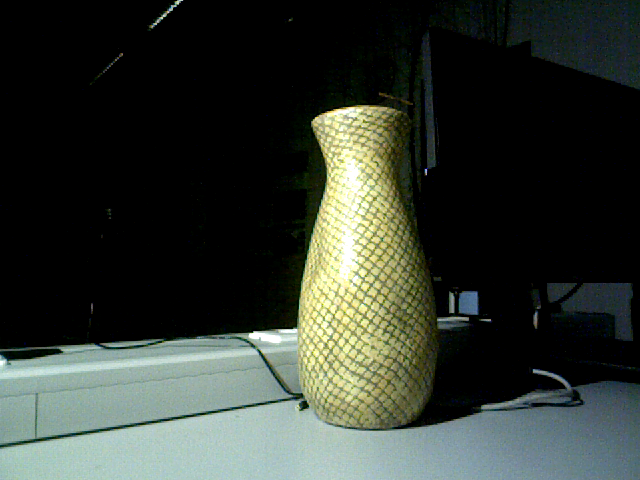
\includegraphics[width=0.23\linewidth]{figures/methodology/robust_setup1.png}}
\subfigure{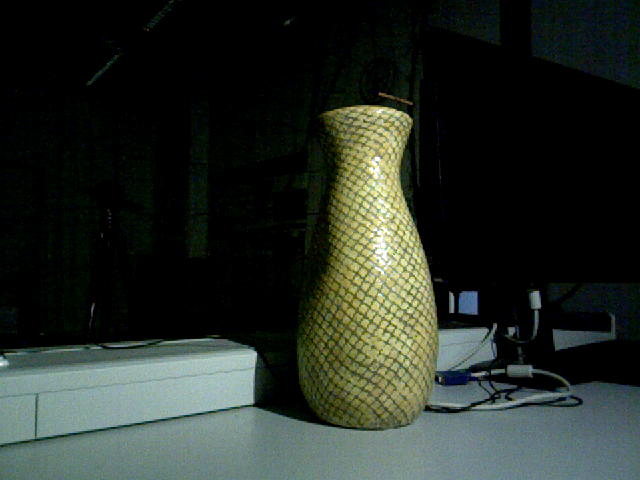
\includegraphics[width=0.23\linewidth]{figures/methodology/robust_setup2.png}}
\subfigure{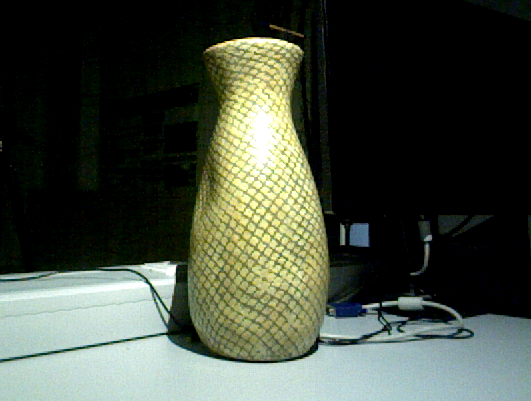
\includegraphics[width=0.23\linewidth]{figures/methodology/robust_setup3.png}}
\subfigure{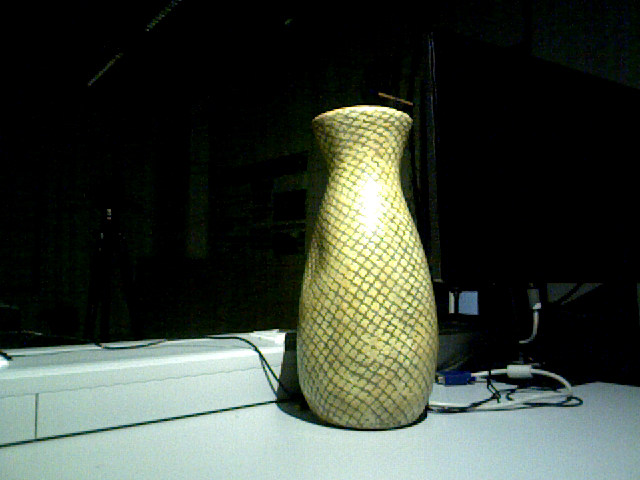
\includegraphics[width=0.23\linewidth]{figures/methodology/robust_setup4.png}}
\caption{Illustrations for the obtained color images of a vase from various light directions with a white LED light.}
\label{fig:robust_setup}
\end{figure}
 
{\color{red} put a real-world albedo estimate case that RGBD-fusion fails but our method works}


%----------------------------------------------
\subsection{Algorithm details}
%----------------------------------------------
Since we don't control with RGB LED lights anymore but one white light, the ratio model in Eq.~\ref{eq:ratio_rg_sh1} is not applicable anymore, so we need to use the standard 1st-order SH model described in Eq.~\ref{eq:rgbd_light_model} again to construct the input color images.

Again, the proposed algorithm consists of three parts: light estimation, albedo estimation and depth enhancement. 
We need to iteratively update the light directions, color albedo and the depth, but unlike the RGB ratio model method, we don't need to have an initial estimated light and albedo beforehand.
Instead, we can just assume the albedo to be 1 everywhere at the beginning and then start refining everything reiteratively in the loop, as shown in Alg.~\ref{alg:robust}.

First of all, the SFS model we use for the proposed method is still from Eq.~\ref{eq:rgbd_light_model}, so the corresponding SFS minimization problem now becomes:
%$$$$$$$$$$$$$$$$$
\begin{equation}
    \sum_{i} \sum_{c} \mathop{\sum \sum}_{(x,y) \in \mathcal{M}} |\rho_c(x,y) \mathbf{s}_{i,c}^\top\tilde{\mathbf{n}}(x,y) - I_{i,c}(x,y)|^2 
\end{equation}
%$$$$$$$$$$$$$$$$$
$c\in\{R,G,B\},\; i\in\{ 1, \cdots, n\}$, where $n$ stands for the total number of varying light directions.
A simplified version of the SFS energy is:
%$$$$$$$$$$$$$$$$$
\begin{equation}
    \sum_{i} \sum_{c} \lVert\rho_c \cdot \tilde{\mathbf{n}}\mathbf{s}_{i,c} -  I_{i,c} \rVert_2^2 
\end{equation}

Now the overall energy for our proposed robust lighting variation method is characterized as:

%$$$$$$$$$$$$$$$$$
\begin{equation}\label{eq:robust_energy}
    E(\rho, z, \mathbf{s}) = \sum_{i} \sum_{c} \lVert \rho_c \cdot \tilde{\mathbf{n}}(z)\mathbf{s}_{i,c}  - I_{i,c}\rVert_2^2  + \lambda_{z}\lVert z - z_0 \rVert_2^2
\end{equation}
%$$$$$$$$$$$$$$$$$
As we can notice, the new overall energy is extremely simple with only one SFS term and one depth fidelity term, no any regularization terms for the albedo or depth estimation.
And we have found out that $\lambda_z = 0.01$ works really well for all cases, which means our system can be used by anybody easily without problems.

\textbf{Light estimation}
In each iteration, we first freeze the albedo and the surface normal and then refine the SH parameters for all input images from the overall energy in Eq.~\ref{eq:robust_energy}.
%%$$$$$$$$$$$$$$$$$
%\begin{equation}\label{eq:robust_light_estimate}
%    \min_{\mathbb{S}_c} \; \sum_{c} \lVert \mathbb{I}_c - \rho_c \mathbb{S}_{c}\tilde{\mathbf{n}}\rVert_2^2
%\end{equation}
%$$$$$$$$$$$$$$$$$
To estimate the light with the simple least squares, we need to reshape the SFS term to a linear problem with the SH light as the argument. 

First of all, to further simplify the energy, we define $\mathbb{I}_c$ and $\mathbf{S}_c$ as:
%$$$$$$$$$$$$$$$$$
\begin{equation}\label{eq:robust_energy_prepare}
\mathbb{I}_c = \begin{pmatrix} I_{1,c} \\ \vdots \\ I_{n,c} \end{pmatrix}  \; \; \mathbf{S}_c = \begin{pmatrix} \mathbf{s}_{1,c} \\ \vdots \\ \mathbf{s}_{n,c} \end{pmatrix}
\end{equation}
%$$$$$$$$$$$$$$$$$
$\mathbb{I}_c \in \mathbb{R}^{mn}, \mathbf{S}_c \in \mathbb{R}^{4n}$.
And then we define a multiplication operator $\odot$ between any matrix $\mathbf{A}$ and vector $\mathbf{b}$ with the same number of rows, $\mathbf{C = A \odot b}$.
$\mathbf{C}$ is the result of the element-wise multiplication between each column of $\mathbf{A}$ and $\mathbf{b}$.
Now we have a vector $\rho_c\in \mathbb{R}^m$ and a matrix $\tilde{\mathbf{n}} \in \mathbb{R}^{m \times 4}$, where $m$ represents the number of pixel inside the mask $\mathcal{M}$.
So we repeat the resulted matrix $\tilde{\mathbf{n}} \odot \rho_c$ on the diagonal of a big sparse matrix $\mathbf{A}_{\mathbb{S}_c} \in \mathbb{R}^{mn \times 4n}$, whose structure is illustrated in Fig.~\ref{fig:robust_matrix1}.
The Eq.~\ref{eq:robust_energy} now is reformulated as:
%$$$$$$$$$$$$$$$$$
\begin{equation}\label{eq:robust_light_estimate2}
    \min_{\mathbf{S}_c} \; \sum_{c} \lVert \mathbf{A}_{\mathbf{s}_c}\mathbf{S}_c  - \mathbb{I}_c \rVert_2^2
\end{equation}
%$$$$$$$$$$$$$$$$$

\textbf{Albedo estimation}
Similar to the light estimation, we need to reshape the SFS term in the overall energy in order to solve with least squares.
The energy for the albedo estimation from the overall energy looks like this:
%$$$$$$$$$$$$$$$$$
\begin{equation}\label{eq:robust_albedo_estimate}
	\min_{\rho_c} \; \sum_{c}\lVert \mathbf{A}_{\rho_c}\rho_c - \mathbb{I}_c \rVert^2_2 
\end{equation}
%$$$$$$$$$$$$$$$$$
$ \mathbf{A}_{\rho_c} \in \mathbb{R}^{mn \times m}$ is the stack of $n$ diagonal matrices $\text{diag}(\tilde{\mathbf{n}} \cdot \mathbf{s}_{i,c})$, where $\text{diag} : \mathbb{R}^m \rightarrow \mathbb{R}^{m\times m}, i \in \{1, \cdots, n\}$.
A toy example of $\mathbf{A}_{\rho_c}$ with $n=6$ is illustrated in Fig.~\ref{fig:robust_matrix2}.

\begin{figure}[!htbp]
\centering
\subfigure[An example of $\mathbb{A}_{\mathbb{S}_c}$ with $n = 6$. The yellow part represents the repetition of matrix $\tilde{\mathbf{n}} \odot \rho_c$]{\label{fig:robust_matrix1}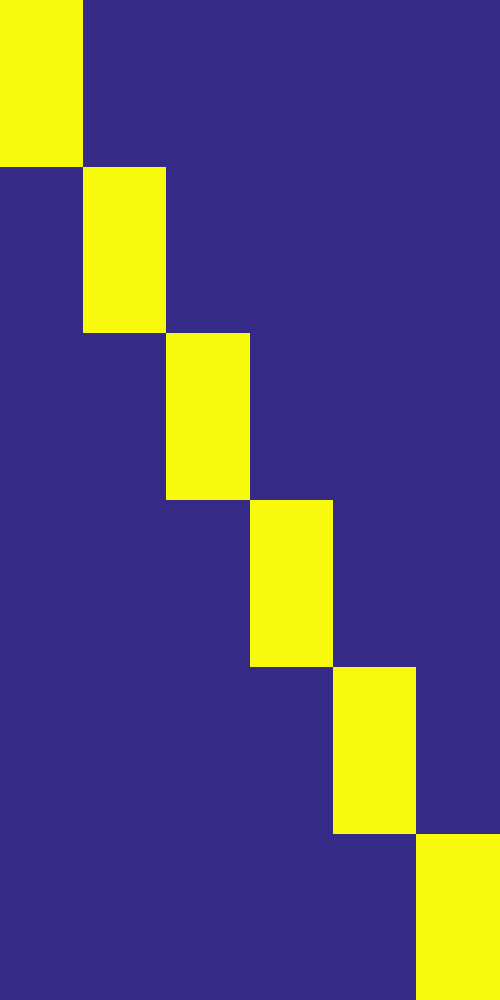
\includegraphics[width=0.3\linewidth]{figures/methodology/As_matrix.pdf}}
\quad
\subfigure[An example of $\mathbb{A}_{\rho_c}$ with $n = 6$. Every yellow line represents $\text{diag}(\tilde{\mathbf{n}} \cdot \mathbf{s}_{i,c})$]{\label{fig:robust_matrix2}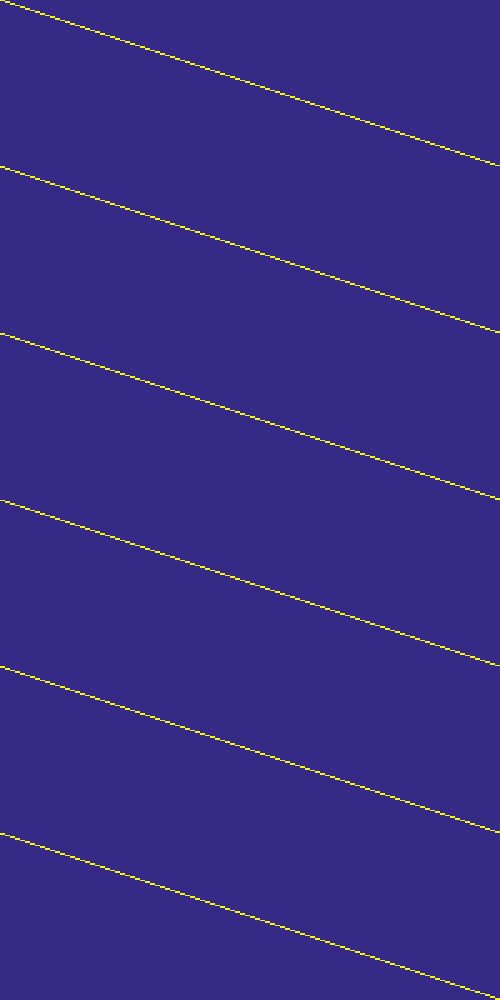
\includegraphics[width=0.3\linewidth]{figures/methodology/Ap_matrix.pdf}}

\caption{Illustrations for the structures of the matrices $\mathbb{A}_{\mathbb{S}_c}$ and $\mathbb{A}_{\rho_c}$. The number of different light conditions is $n = 6$.}
\label{fig:robust_matrix}
\end{figure}

\textbf{Depth enhancement}
After having the estimated light and the color albedo, we can continue refining the depth.
Again, we need to rearrange the energy function with the depth $z$ as the argument.
First, let us start from the simplest case and consider one pixel in one of the input images.
If we expand Eq.~\ref{eq:rgbd_light_model} with the the perspective projection normal in Eq.~\ref{eq:ratio_normal}, we have:
%$$$$$$$$$$$$$$$$$
\begin{equation}
    I(x,y) = \rho(x,y) \cdot \; 
    \begin{pmatrix}
        l^1 & l^2 & l^3 
    \end{pmatrix}
     \begin{pmatrix}
         fz_x(x,y)\\
         fz_y(x,y)\\
         -1 - (x - x_0)z_x(x,y) - (y - y_0)z_y(x,y)
     \end{pmatrix}/ d(x,y)
     + \rho(x,y) \cdot \varphi   
\end{equation}
%$$$$$$$$$$$$$$$$$
where $d = \sqrt{(fz_x(x,y))^2 + (fz_y(x,y))^2 + (-1 - (x - x_0)z_x(x,y) - (y - y_0)z_y(x,y))^2}$ is a normalizer.
After rearranging, we have:
 %$$$$$$$$$$$$$$$$$
\begin{equation}
    \frac{l^1f - l^3(x-x_0)}{d(x,y)}z_x(x,y) + \frac{l^2f - l^3(y-y_0)}{d(x,y)}z_y(x,y) = I(x,y) + \frac{l^3}{d(x,y)} - \rho(x,y)\varphi
\end{equation}
 %$$$$$$$$$$$$$$$$$
If we extend this to the whole pixel in the mask $\mathcal{M}$, the equation becomes:
 %$$$$$$$$$$$$$$$$$
\begin{equation}\label{eq:robust_depth1}
    \frac{l^1f - l^3\tilde{x}}{d} \cdot z_x + \frac{l^2f - l^3\tilde{y}}{d} \cdot z_y = I + \frac{l^3}{d} - \varphi \cdot \rho
\end{equation}
Provided we have the gradient matrices in $x$ and $y$ directions denoted roughly as:
 %$$$$$$$$$$$$$$$$$
\begin{equation}
D_x = \begin{pmatrix}
-1 & 1 & 0 &\cdots & 0 & 0 \\
0 & -1 & 1 &\cdots &  0 & 0 \\
\vdots & \vdots & \ddots & \ddots & \vdots & \vdots \\
0 & 0 & 0 & \cdots & -1 & 1
\end{pmatrix}_{m\times m}
\quad
D_y = \begin{pmatrix}
-1 & 0 & \cdots & 0 \\
1 & -1 & \cdots & 0 \\
0 & 1 & \ddots & 0 \\
\vdots & \vdots & \ddots & \vdots\\
0 & 0 & \cdots & -1\\
0 & 0 & \cdots & 1
\end{pmatrix}_{m\times m}
\end{equation}
 %$$$$$$$$$$$$$$$$$
Then Eq.~\ref{eq:robust_depth1} becomes:
 %$$$$$$$$$$$$$$$$$
\begin{equation}\label{eq:robust_depth2}
        [\text{diag}(\frac{l^1f - l^3\tilde{x}}{d}) D_x + \text{diag}(\frac{l^2f - l^3\tilde{y}}{d}) D_y] z = I + \frac{l^3}{d} - \varphi \cdot \rho
\end{equation}
 %$$$$$$$$$$$$$$$$$
This is the linear equation for one image. 
Now we define our $\mathbf{A}_z$ and $\mathbf{b}_z$ for our system:
 %$$$$$$$$$$$$$$$$$
\begin{equation}\label{eq:robust_depth3}
\begin{split}
    \mathbf{A}_{z_c} &= 
        \begin{pmatrix}    
            \text{diag}(\frac{l^1_{1,c}f - l^3_{1,c}\tilde{x}}{d_1}) D_x + \text{diag}(\frac{l^2_{1,c}f - l^3_{1,c}\tilde{y}}{d_1}) D_y \\
            \vdots \\
            \text{diag}(\frac{l^1_{n,c}f - l^3_{n,c}\tilde{x}}{d_n}) D_x + \text{diag}(\frac{l^2_{n,c}f - l^3_{n,c}\tilde{y}}{d_n}) D_y \\
        \end{pmatrix}_{mn \times m}
\\
    \mathbf{b}_{z_c} &=     
        \begin{pmatrix}    
            I_{1,c} + \frac{l^3_{1,c}}{d_{1}} - \varphi_{1,c} \cdot \rho_{c} \\
            \vdots\\
            I_{n,c} + \frac{l^3_{n,c}}{d_{n}} - \varphi_{n,c} \cdot \rho_{c} \\
        \end{pmatrix}_{mn \times 1}    
\end{split}
\end{equation}
 %$$$$$$$$$$$$$$$$$
 It worths mentioning that in each iteration, we freeze $d$ with $z$ from last iteration, so the non-linearity is solved.
 Finally, we have stack $\mathbf{A}_{z_c}$ and $\mathbf{b}_{z_c}$ for each channel $c\in\{R,G,B\}$:
 %$$$$$$$$$$$$$$$$$
 \begin{equation}
     \mathbf{A}_z = 
         \begin{pmatrix}
             \mathbf{A}_{z_R}\\
             \mathbf{A}_{z_G}\\
             \mathbf{A}_{z_B}
         \end{pmatrix},\quad
     \mathbf{b}_z = 
         \begin{pmatrix}
             \mathbf{b}_{z_R}\\
             \mathbf{b}_{z_G}\\
             \mathbf{b}_{z_B}
         \end{pmatrix}         
 \end{equation}
 %$$$$$$$$$$$$$$$$$
After all the derivations, we finally model our energy for the depth enhancement as:
 %$$$$$$$$$$$$$$$$$
 \begin{equation}\label{eq:robust_depth_estimate}
	\min_{z} \; \lVert  \mathbf{A}_{z}z - \mathbf{b}_z\rVert^2_2 + \lambda_{z}\lVert z - z_0 \rVert_2^2
\end{equation}
 %$$$$$$$$$$$$$$$$$
The structure of the proposed algorithm is described below:
\begin{algorithm}[!htbp]
	\begin{algorithmic}[1] 
  		\caption{\textbf{Robust Light Variation Model Method}}
		\label{alg:robust}
		 \renewcommand{\algorithmicrequire}{\textbf{Input:}}
		 \renewcommand{\algorithmicensure}{\textbf{Output:}}
		 \REQUIRE Initial depth image $z_0$, RGB image $I$, mask, focal length, principle point
		 \vspace{1.8mm}
		 \STATE t = 1, $z^{(t-1)} = z_0$, $\rho^{(0)}_R, \rho^{(0)}_G, \rho^{(0)}_B = 1$
		 \vspace{1.8mm}
		  \WHILE {$ \frac{\Vert E(\rho^{(t)}, z^{(t)}, \mathbf{s}^{(t)}) - E(\rho^{(t-1)}, z^{(t-1)}, \mathbf{s}^{(t)})\Vert}{E(\rho^{(t-1)}, z^{(t-1)}), \mathbf{s}^{(t-1)}} > \epsilon$}
		       \vspace{1.8mm}
		        \STATE $\mathbf{s}^{(t)} = \argmin \limits_{\rho} E(\rho^{(t-1)}, z^{(t-1)})$ \COMMENT{Eq.~\ref{eq:robust_light_estimate2}}
			\STATE $\rho^{(t)} = \argmin \limits_{\rho} E(z^{(t-1)}, \mathbf{s}^{(t)})$ \COMMENT{Eq.~\ref{eq:robust_albedo_estimate}}
			  \STATE $z^{(t)} = \argmin \limits_{z} E(\rho^{(t)}, z^{(t-1)}, \mathbf{s}^{(t)})$ \COMMENT{Eq.~\ref{eq:robust_depth_estimate}}
			  \vspace{1.8mm}
		          \STATE $t := t + 1$
		 \vspace{1.8mm}
		  \ENDWHILE
		  \ENSURE  Refined depth image $z^{(t)}$ and albedo $\rho^{(t)}$
	\end{algorithmic}
\end{algorithm}

%----------------------------------------------
\subsection{When super-resolution meets depth refinement}
%----------------------------------------------
For most of the well-known comsumer RGB-D cameras, the depth resolution is far smaller than the RGB resolution.
For instance, ASUS XtionPro Live can acquire $1280\times 1024$ RGB images and $640\times 480$ depth images. Microsoft Kinect 2.0 owns $1920\times1080$ RGB resolution but only $512\times424$ depth one, and Intel RealSense R200 has a $1920\times1080$ RGB camera while the depth reoslution is $640\times 480$.
It would be very useful if we can not only refine the depth map in its original scale, but close to the RGB resolution.  

In this section, we will present our approach of the combination of the photometric stereo and super-resolution, with the help of which we will provide satisfying high-quality and high-resolution depth maps. 

The scale factor between the RGB and depth image is around $2$ for ASUS XtionPro Live, so we can at least enlarge our map two times larger than the original size, which means the refined depth resolution will be $1280\times960$.
 And we assume that the input depth image has been registered well (done easily with OpenNI) such that the upsampled depth $Z$ is aligned with the large RGB image after simple interpolation.

The whole process follows our Robust lighting variation model method described in Alg.~\ref{alg:robust}.
In the light, albedo estimation part, the energy in Eq.~\ref{eq:robust_light_estimate2} and Eq.~\ref{eq:robust_albedo_estimate} are direct used. we only replace the surface normal $\mathbf{n}(z)$ with $\mathbf{N}(Z)$ when we build $\mathbf{A}_{\mathbf{s}_c}$ and $\mathbf{A}_{\rho_c}$. 
When refining the depth with Eq.~\ref{eq:robust_depth_estimate}, $Z$ is also used to replace $z$ during the construction of $\mathbf{A}_z$ and $\mathbf{b}_z$, and now denoted by $\mathbf{A}_Z$ and $\mathbf{b}_Z$.
 
 \begin{figure}[!htbp]
\centering
\subfigure[One input image $(960\times1280)$]{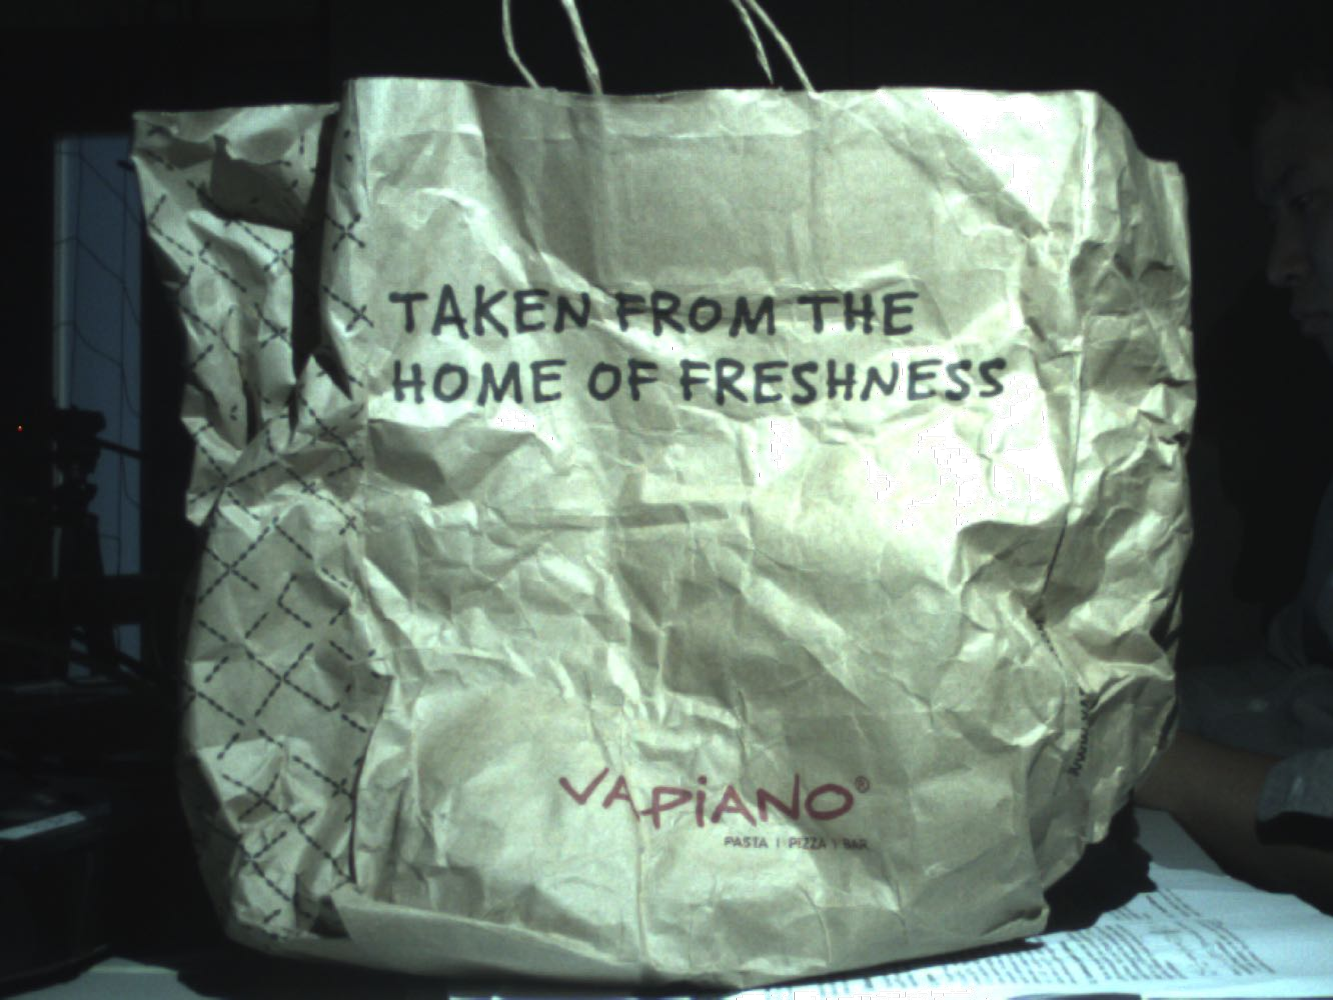
\includegraphics[width=0.32\linewidth]{figures/methodology/sr_rgb_big.pdf}}
\subfigure[Estimated albedo $(960\times1280)$]{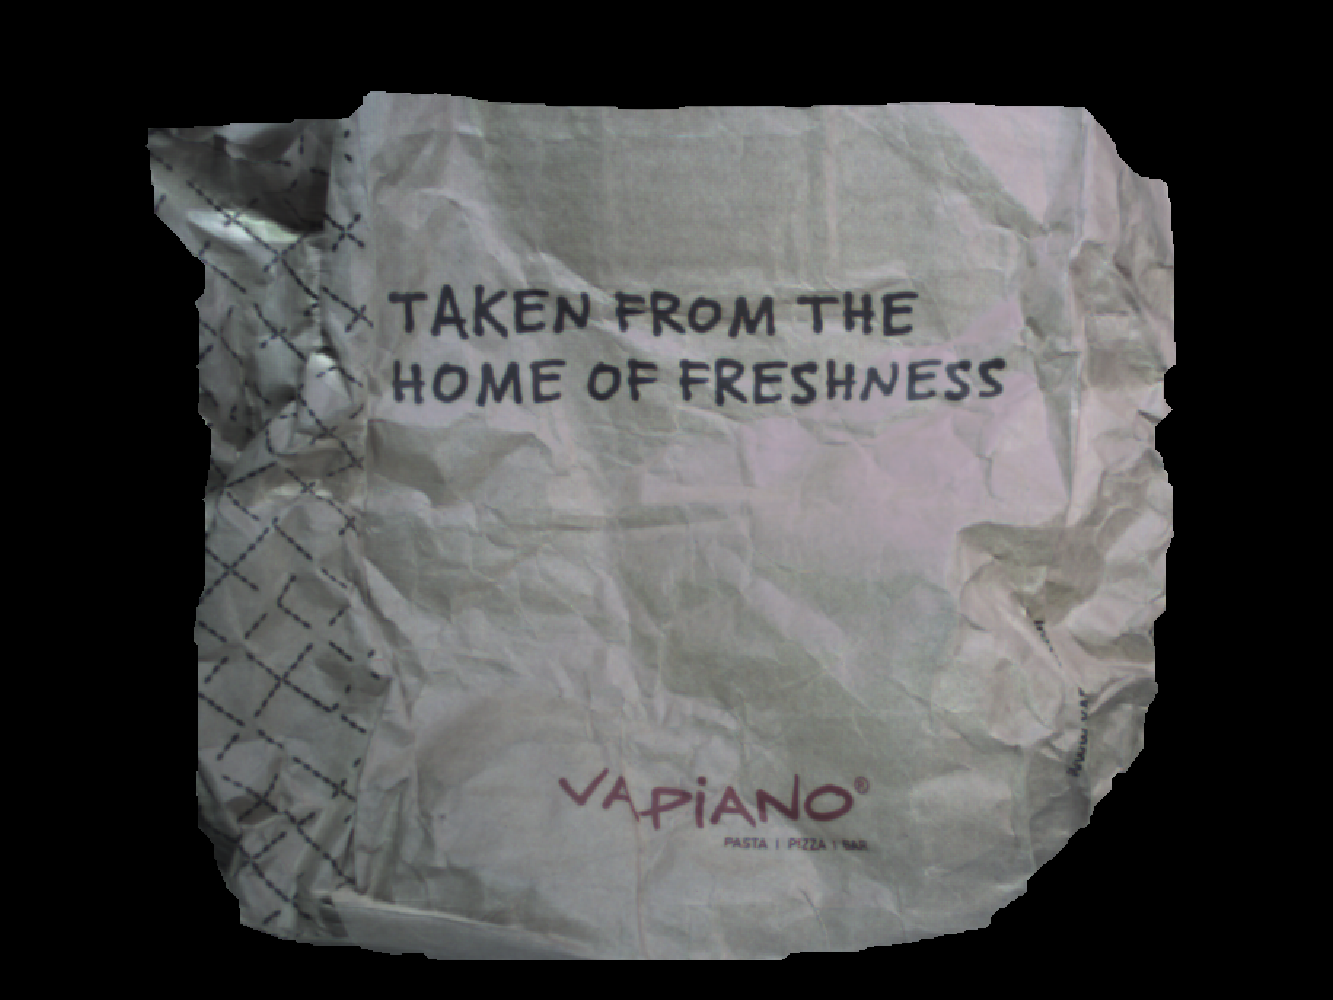
\includegraphics[width=0.32\linewidth]{figures/methodology/sr_albedo.pdf}}
\subfigure[Estimated normal$(960\times1280)$]{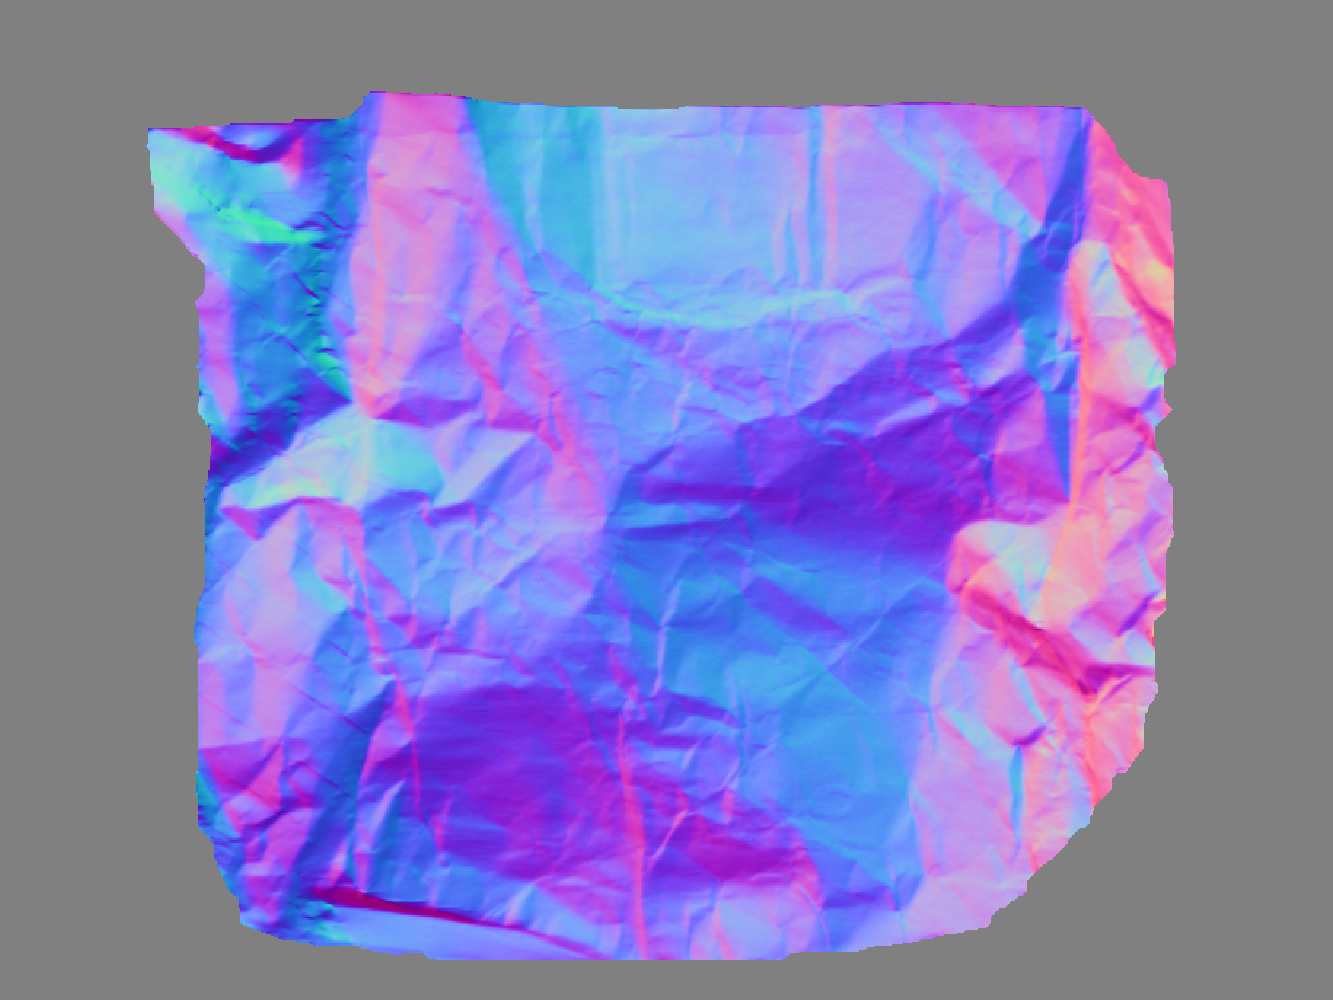
\includegraphics[width=0.32\linewidth]{figures/methodology/sr_normal.pdf}}
\subfigure[Input depth image $(480\times640)$]{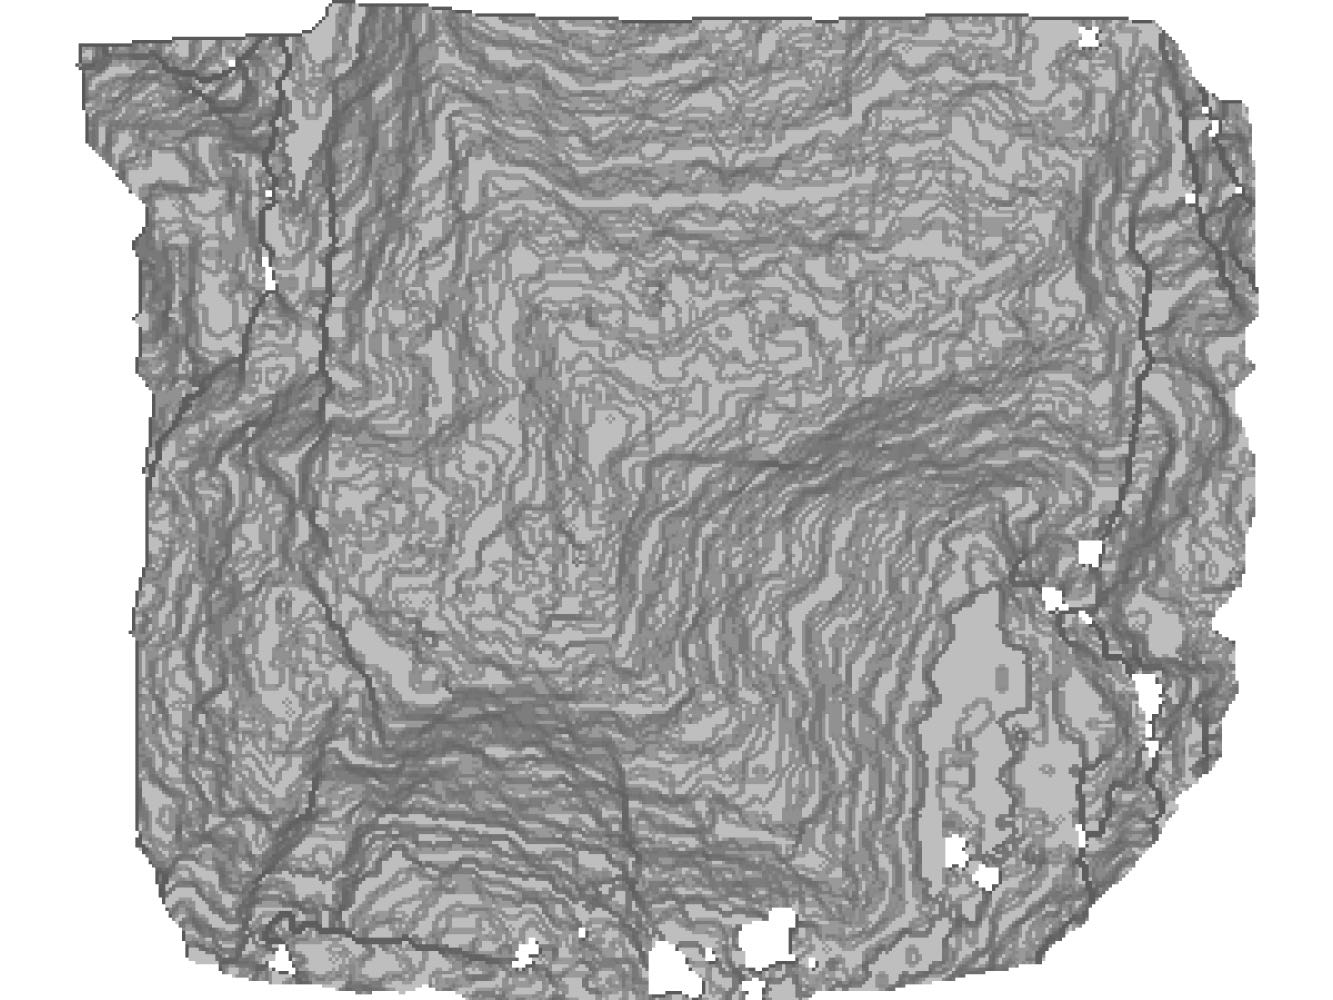
\includegraphics[width=0.23\linewidth]{figures/methodology/sr_shape_before.pdf}}
\quad
\subfigure[Smoothed depth image $(480\times640)$]{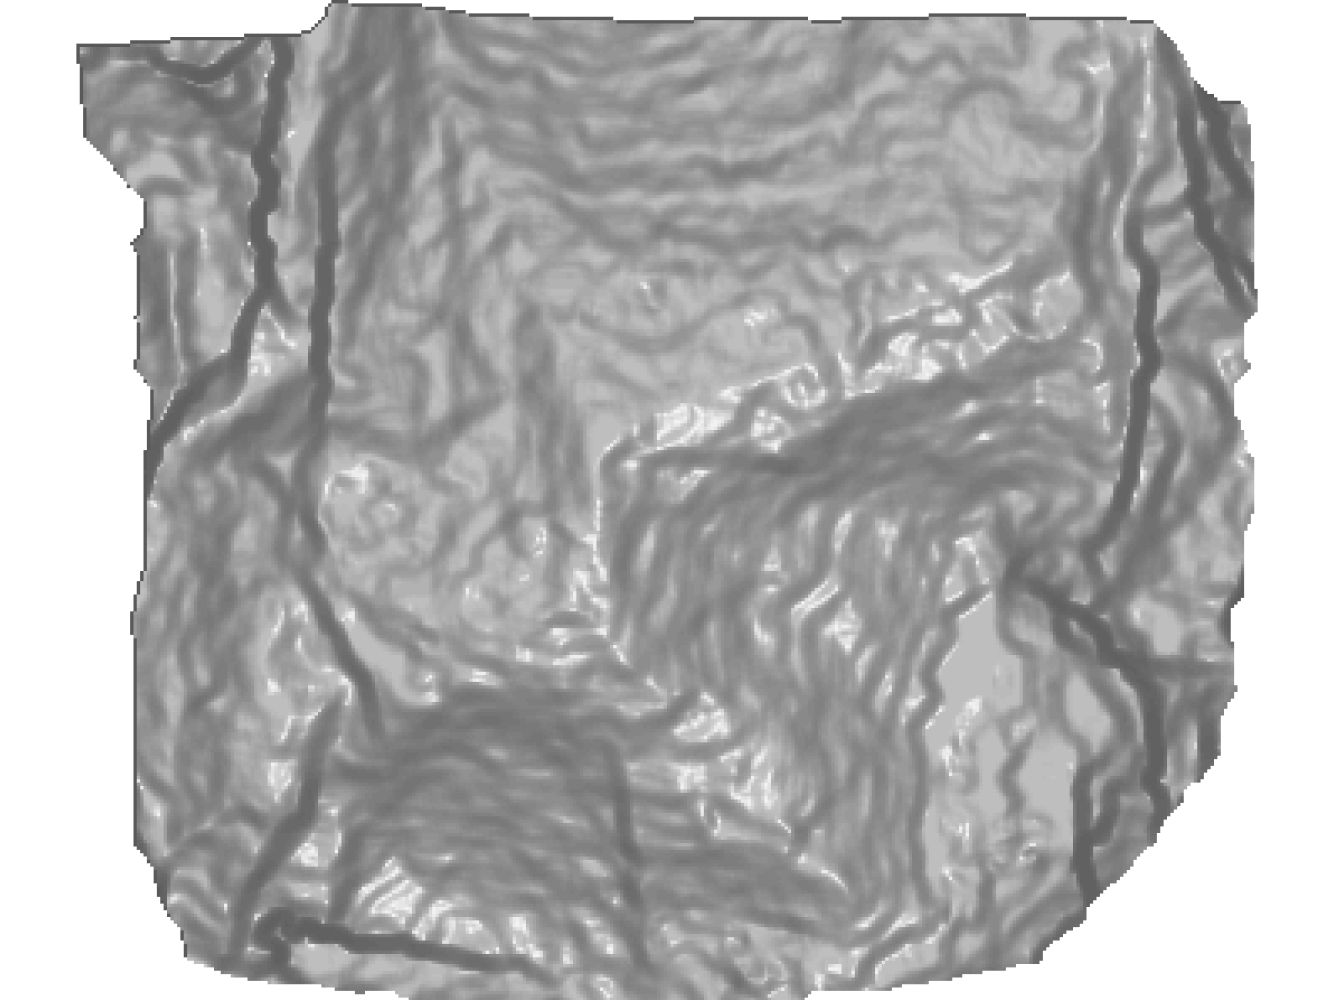
\includegraphics[width=0.23\linewidth]{figures/methodology/sr_shape_smooth.pdf}}
\subfigure[Refined super-resolution depth $(480\times640)$]{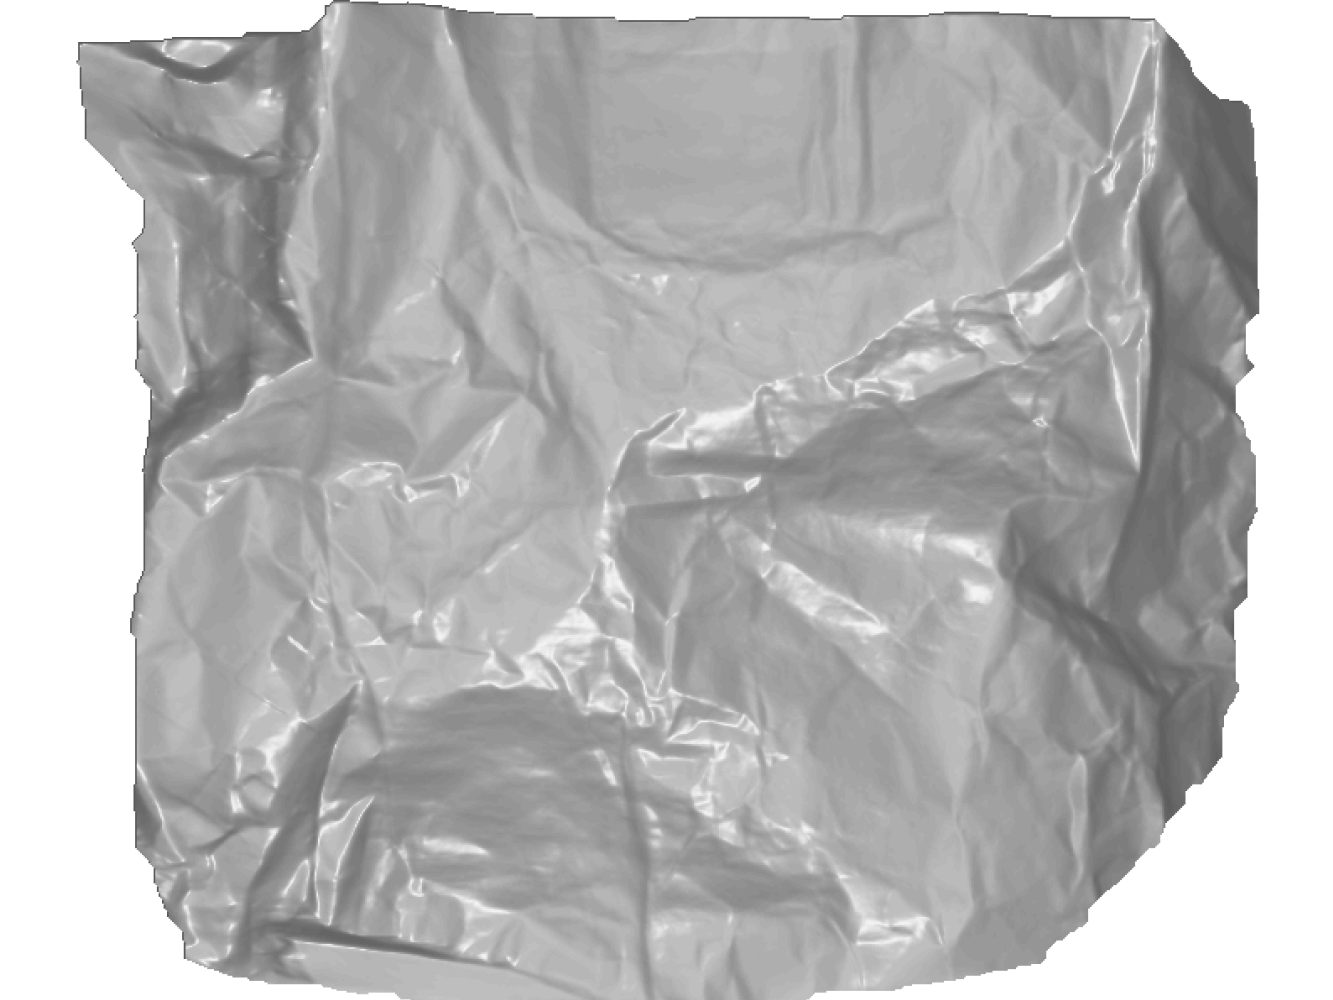
\includegraphics[width=0.46\linewidth]{figures/methodology/sr_shape_after.pdf}}
\caption{Results of the super-resolution depth of a paper bag. Input depth size is $480\times 640$, and the refined depth's is $960 \times 1280$.}
\label{fig:robust_sr}
\end{figure}
 
For the data fidelity term, it needs to be changed and adapted to the input small depth $z_0$ with a downsampling kernal $K \in \mathbb{R}^{m\times M}$, where $M$ and $m$ represent the number of pixel within the big mask and the small mask respectively.
The super-resolution depth refinement energy now is changed to:
 %$$$$$$$$$$$$$$$$$
 \begin{equation}\label{eq:robust_depth_estimate}
	\min_{Z} \; \lVert  \mathbf{A}_{Z}Z - \mathbf{b}_Z\rVert^2_2 + \lambda_{z}\lVert K\cdot Z - z_0 \rVert_2^2
\end{equation}
 %$$$$$$$$$$$$$$$$$
%%%%%%%%%%%%%%%%%%%%%%%%%%%%%%%%%%%%%%%%%%%%


\chapter{Results and Evaluation} \label{chap:result}
%{\color{red}Give some introduction, the structure of this chapter.}
\textbf{Parameter setup}
First we need to specify the parameters we used throughout the whole evaluation part. 
The default parameters are applied for the RGBD-Fusion method, which has 8 in total. 
It should be mentioned that, since both proposed methods don't have smoothness term for the depth enhancement, the $\lambda_z^2$ in RGBD-Fusion and $\lambda_l$ in our implementation RGBD-Fusion Like method are set to 0 for the sake of fairness comparison.
Only during the quantitative evalution, we want to illustrate the importance of this smoothness term so the $\lambda_z^2$ and $\lambda_l$ are set to the values in table~\ref{tab:parameter_setup}.
\begin{table}[!ht]
\caption{Parameters of all the methods throughout all the experiments.}
\label{tab:parameter_setup}
\centering
\begin{tabular}{|m{4cm} |m{1.5cm} |m{7cm}|}
\hline
\multicolumn{1}{|c|}{Method}                               & \multicolumn{1}{c|}{Total number} & \multicolumn{1}{c|}{Parameters}                                                                                                                                          \\ \hline
RGBD-Fusion~\cite{or2015rgbd} & \multicolumn{1}{c|}{8}            &{$\lambda_\rho = 0.1, \lambda_\beta^1 = 0.1, \lambda_\beta^2 = 0.1, \tau = 0.05, \sigma_c = \sqrt{0.05}, \sigma_d = \sqrt{50}, \lambda_z^1 = 0.004, \lambda_z^2 = 0.0075$} \\ \hline
RGBD-Fusion Like method (Eq.~\ref{eq:rgbd_energy})                    & \multicolumn{1}{c|}{5}             & {$\lambda_{\rho} = 10, \sigma_I = \sqrt{0.05}, \sigma_z = \sqrt{50}, \lambda_z = 500, \lambda_l = 2$}                                                                                                                                                                         \\ \hline
Proposed I: RGB Ratio model (Eq.~\ref{eq:ratio_energy})                            & \multicolumn{1}{c|}{4}             & $\lambda_{\rho}^1 = 10^{15}, \lambda_{\rho}^2 = 10^{13}, \sigma_c = 100, \lambda_z = 100$                                                                                                                                                                                                                                                                                                                                                  \\ \hline
Proposed II: Robust Multi-Light  (Eq.~\ref{eq:robust_energy})                        & \multicolumn{1}{c|}{1}            & $\lambda_z = 100$                                                                                                                                                                          \\ \hline
\end{tabular}
\end{table}

%%%%%%%%%%%%%%%%%%%%%%%%%%%%%%%%%%%%%%%%%%%%
\section{Quantitative Evaluation}
%%%%%%%%%%%%%%%%%%%%%%%%%%%%%%%%%%%%%%%%%%%%


%-------------------------------------------------------------------------------
\subsection{Data generation}
%-------------------------------------------------------------------------------
In order to quantitatively validate the performance of our proposed methods and our implementation of the RGBD-Fusion, we use the well-known "The Joyful Yell" dataset with 3 point light sources and ambient lights. 

To simulate the natural scene illumination, we assume the RGB lighting as frontal directions, so the first-order SH parameters are modelled as:
\begin{equation*}
    \mathbf{s}_R = \mathbf{s}_G = \mathbf{s}_B = \begin{bmatrix} 0 & 0& -1 & 0.2\end{bmatrix}^\top
    \qquad
    \raisebox{-0.5cm}{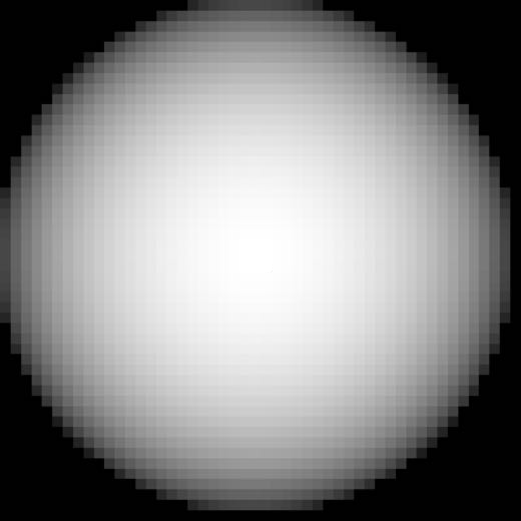
\includegraphics[height=0.1\textwidth]{figures/result/light9.pdf}}
\end{equation*}

And then, in order to reproduce the LED configuration for the proposed RGB ratio model, we define the 3 lighting directions as:
\begin{equation*}
    \begin{split}
        \mathbf{s}_R &= \begin{bmatrix} 0 &0 &-1 &0.15\end{bmatrix}^\top\\
        \mathbf{s}_G &= \begin{bmatrix} 0.3 & 0.2 & -1 & 0.25\end{bmatrix}^\top\\
        \mathbf{s}_B &= \begin{bmatrix} -0.2 & 0.3 & -1 & 0.2\end{bmatrix}^\top\\
    \end{split}
    \qquad\qquad\quad
    \raisebox{-0.7cm}{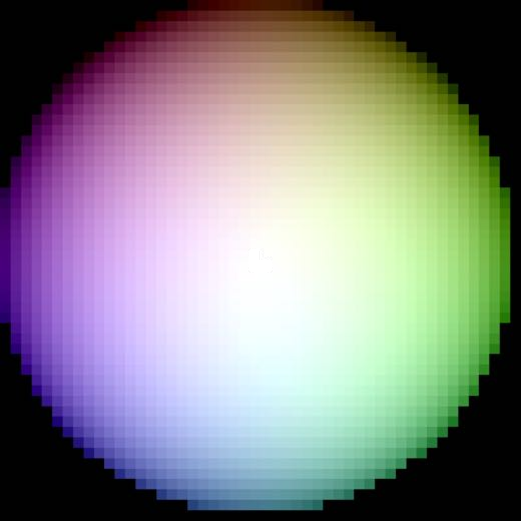
\includegraphics[height=0.1\textwidth]{figures/result/light_color.pdf}}
\end{equation*}
Finally, we need to produce a sequence of same images with various directional lights for our robust multi-light model.
A "lighting" matrix $L$ and the corresponding positions of 10 point light sources can be illustrated as below, where red points represent the light positions.
\begin{equation*}
\begin{split}
L = 
    \begin{pmatrix}
        0.5 & 0 & -1 & 0.2\\
        0.3 & 0.4 & -1 & 0.2\\
        0 & 0.5 & -1 & 0.2\\
        -0.4 & 0.3 & -1 & 0.2\\
        -0.5 & 0 & -1 & 0.2\\
        -0.3 & -0.4 & -1 & 0.2\\
        0 & -0.5 & -1 & 0.2\\
        0.4 & -0.3 & -1 & 0.2\\
        0 & 0 & -1 & 0.2\\
        0.45 & 0.2 & -1 & 0.2\\
    \end{pmatrix}^\top 
    \qquad 
    &\raisebox{-2.8cm}{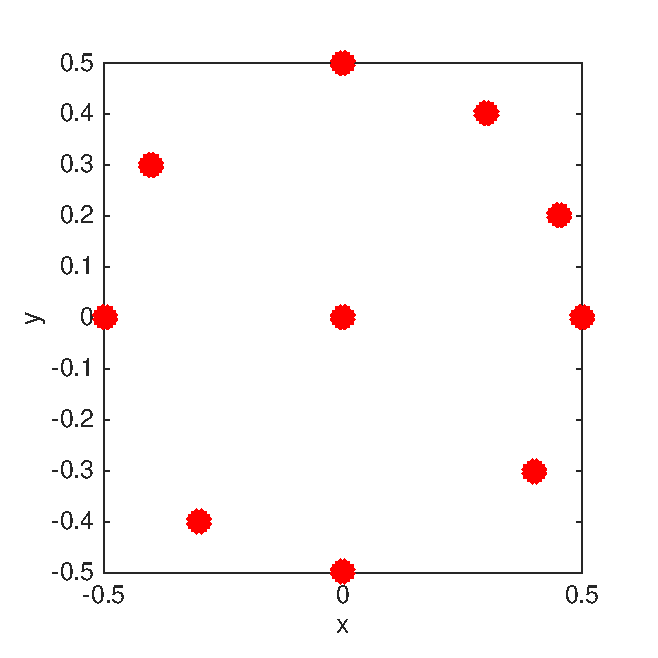
\includegraphics[height=0.4\textwidth]{figures/result/example_multi_light.eps}}\\
    \raisebox{-0.4cm}{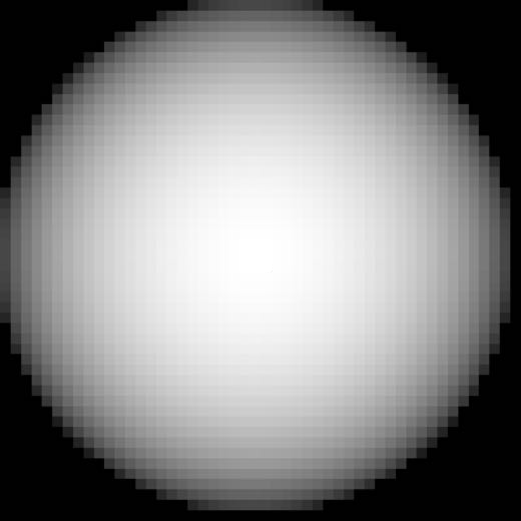
\includegraphics[height=0.1\textwidth]{figures/result/light9.pdf}}    
    \raisebox{-0.4cm}{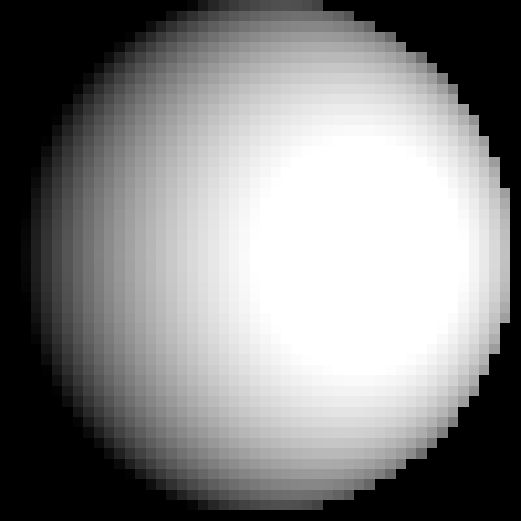
\includegraphics[height=0.1\textwidth]{figures/result/light1.pdf}}
    \raisebox{-0.4cm}{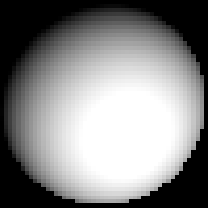
\includegraphics[height=0.1\textwidth]{figures/result/light2.pdf}}
    \raisebox{-0.4cm}{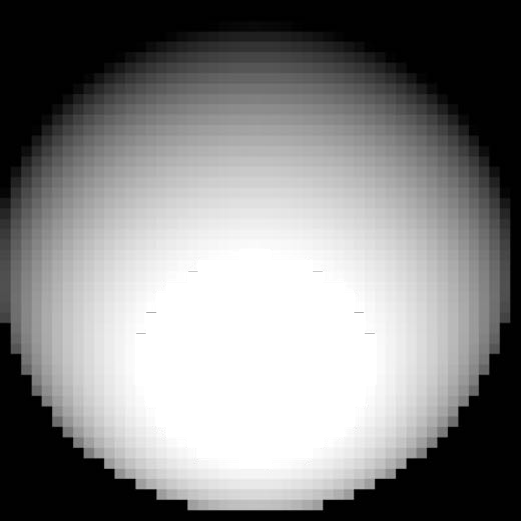
\includegraphics[height=0.1\textwidth]{figures/result/light3.pdf}}
    \raisebox{-0.4cm}{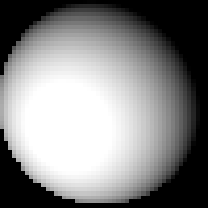
\includegraphics[height=0.1\textwidth]{figures/result/light4.pdf}}
    &\raisebox{-0.4cm}{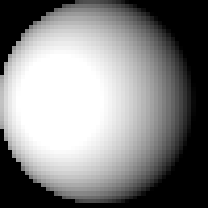
\includegraphics[height=0.1\textwidth]{figures/result/light5.pdf}}
    \raisebox{-0.4cm}{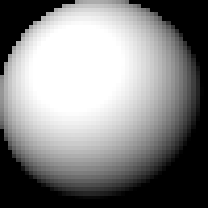
\includegraphics[height=0.1\textwidth]{figures/result/light6.pdf}}
    \raisebox{-0.4cm}{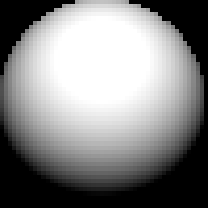
\includegraphics[height=0.1\textwidth]{figures/result/light7.pdf}}
    \raisebox{-0.4cm}{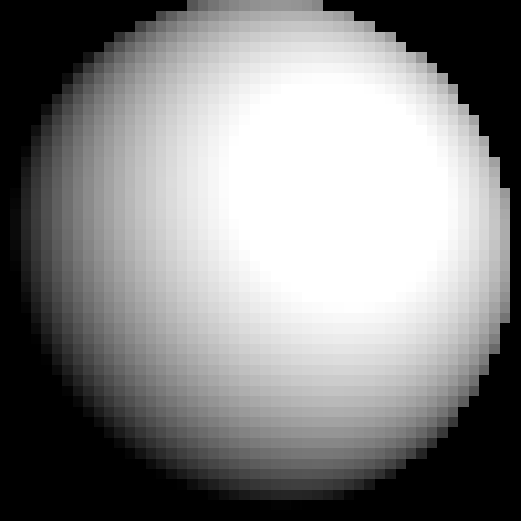
\includegraphics[height=0.1\textwidth]{figures/result/light8.pdf}}
    \raisebox{-0.4cm}{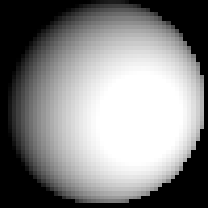
\includegraphics[height=0.1\textwidth]{figures/result/light10.pdf}}
    \end{split}
\end{equation*}
After defining the lightings for various methods, three various albedo scenarios are also considered: 
\begin{itemize}
    \item Red, green and blue piece-wise constant areas
    \item Colorful patterns with a few small details inside\footnote{EBSD map. Image Courtesy of \url{https://mtex-toolbox.github.io/files/doc/EBSDSpatialPlots.html}}
    \item Colorful patterns with complicated details\footnote{1000 Visual Mashups. Image Courtsesy of \url{https://www.flickr.com/photos/qthomasbower/3470650293}}
\end{itemize}


With the 3 different albedos and all the pre-defined lights, we can create the synthetic color images like the first row in Fig.~\ref{fig:result_syn_comp}.

%-------------------------------------------------------------------------------
\subsection{Results Accuracy}
%-------------------------------------------------------------------------------
\textbf{Metrics}
Two metrics have been defined to quantitatively evaluate the performance of depth refinement: root mean square error (RMSE) and mean angular error (MAE).
Since we have already had the input rough depth and the ground truth depth as shown in Fig.~\ref{fig:comp_syn_input}, we can define two metrics as follows.

Assuming $z_g, N_g$ and $z, N$ are the ground truth and the refined depth and normal respectively, $m$ the total number of pixels inside the given mask $\mathcal{M}$ and $i$ the index inside the mask, a loosely definition is: 
\begin{align}
    e_{RMSE} &= \sqrt{\frac{\sum\limits_{i}^{m}{(z(i) - z_g(i))^2}}{m}}\\
    e_{MAE} &= \frac{\sum\limits_{i}^{m} \arccos (N(i) \cdot N_g(i))}{m}
\end{align}
The RMSE reflects refined depth quality, while the MAE illustrates if the refined object's shape is similar to the real one. 
It should be mentioned that $e_{MAE}$ gives values in radians but we convert it to degrees.

\begin{table}[!ht]
\caption{Quantitative evaluations among 4 methods. RMSE and MAE are in pixels and degrees respectively. "No smooth" means no laplacian smoothness term in depth enhancement.}
\vspace{1em}
\label{tab:comp_syn_eval}
\centering
\begin{tabular}{lllllll}
                                       & \multicolumn{2}{c}{Simple RGB}                     & \multicolumn{2}{c}{Pattern}                        & \multicolumn{2}{c}{Complicated Pattern}            \\\hline
Method                                 & \multicolumn{1}{c}{RMSE} & \multicolumn{1}{c}{MAE} & \multicolumn{1}{c}{RMSE} & \multicolumn{1}{c}{MAE} & \multicolumn{1}{c}{RMSE} & \multicolumn{1}{c}{MAE} \\\hline\hline
Input reference                              & 3.3305                   & 16.3096                 & 3.3305                   & 16.3096                 & 3.3305                   & 16.3096                 \\
RGBD-Fusion\cite{or2015rgbd} (no smooth)                       & 3.3418                   & 18.9115                 & 3.3872                   & 27.0026                 & 3.3411                   & 25.6574  		\\
RGBD-Fusion\cite{or2015rgbd} & 3.1751                   & 17.2197                 & 3.1890                   & 18.4722                 & 3.1708                   & 18.0850                 \\ 
Fusion-Like (no smooth)                  & 3.3475                   & 17.5911                 & 3.3459                   & 23.4808                 & 3.3898                   & 35.2610                 \\
Fusion-Like                        & 2.8700                   & 17.1776                 & 2.8749                   & 17.7302                 & 2.8848                   & 19.6452                 \\
RGB ratio model                        & \textbf{1.9437}          & \textbf{5.0574}         & 2.9116                   & 17.5238                 & 3.1006                   & 21.2286                 \\
Robust multi-light model               & 3.4025                   & 6.6640                  & \textbf{1.5794}          & \textbf{1.7368}         & \textbf{1.8424}          & \textbf{2.6815}  \\\hline      
\end{tabular}
\end{table}


According to table~\ref{tab:parameter_setup},~\ref{tab:comp_syn_eval} and Fig.~\ref{fig:result_syn_comp}, there are some interesting observations:
\begin{itemize}
    \item Our RGBD-Fusion Like method uses less parameters than RGBD-Fusion~\cite{or2015rgbd} (5 against 8) but achieves almost the same results as the original paper. 
    \item The Laplacian smoothness term in the depth enhancement energy of RGBD-Fusion method has a huge impact on the refined results. In contrast, both our proposed methods have no smoothness term but gives equal or better results.
    \item Single depth image refinement methods (RGBD-Fusion and RGB ratio model) have a chance to acquire satisfying results only when the albedo is elementary with several big color patches. 
    However, they will fail and give even worse in terms of RMSE and MAE when the albedos get complex. 
    Most of the small details on the albedo of "Pattern" and "Complicate Pattern" cannot be acquired, which leads to the wrong depth estimation.
    This is due to the fact that the albedo estimation in these methods highly relies on the regularization terms which prefers piecewise smooth, but this does not meet the condition of most real-world objects.
    \item It can be effortlessly noticed that our robust multi-light method has a strong ability to handle the cases with extremely complicated albedo. 
    Instead of using any regularization for calculating the albedo, extra images with various light directions solve the overfitting problems of albedo and enable the albedo estimation with only the SFS term (Eq.~\ref{eq:robust_albedo_estimate}).
\end{itemize}




\begin{figure}[!ht]
\centering
\subfigure[Input depth]{\label{fig:robust_matrix1}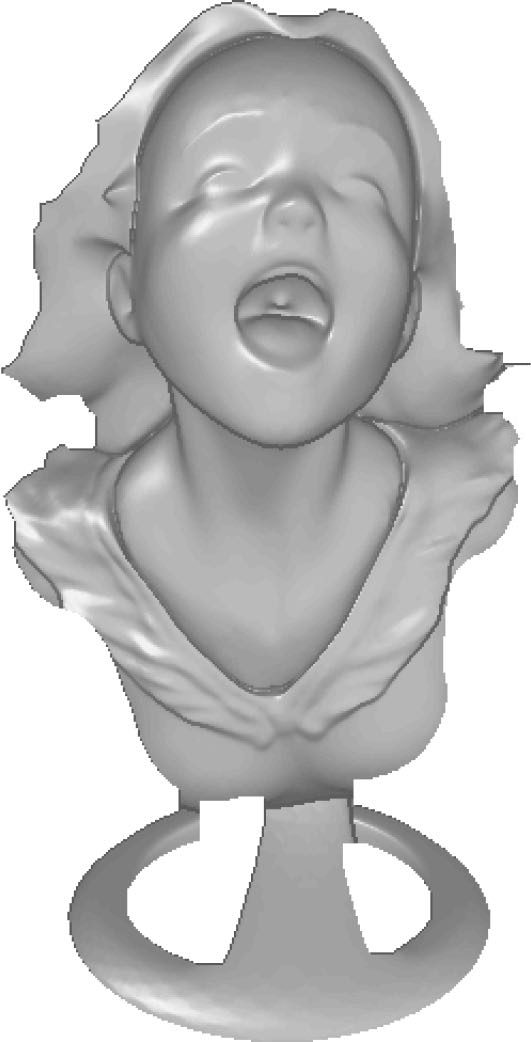
\includegraphics[width=0.2\linewidth]{figures/result/comp_input_shape.pdf}}
\qquad \qquad
\subfigure[Ground truth depth]{\label{fig:robust_matrix2}\includegraphics[width=0.2\linewidth]{figures/result/comp_gt_shape.pdf}}
\caption{The 3D shape of input rough depth and the ground truth depth for the quantitative evalution.}
\label{fig:comp_syn_input}
\end{figure}


\begin{figure}
  % Top row: Ground truth, Image + SH, Image + SH, Image + SH
  \setlength{\tabcolsep}{0.5em} % for the horizontal padding
{\renewcommand{\arraystretch}{0.6}% for the vertical padding
\begin{tabular}{cccc}
%    \multicolumn{2}{c}{\includegraphics[width=0.1\linewidth]{figures/result/comp_robust_pattern_shape.pdf}} &
&
    \includegraphics[height=0.25\linewidth]{figures/result/comp_simple_rgb.pdf}
    \includegraphics[height=0.25\linewidth]{figures/result/comp_simple_albedo.pdf}& 
    \includegraphics[height=0.25\linewidth]{figures/result/comp_pattern_rgb.pdf} 
    \includegraphics[height=0.25\linewidth]{figures/result/comp_pattern_albedo.pdf}& 
    \includegraphics[height=0.25\linewidth]{figures/result/comp_love_rgb.pdf}
    \includegraphics[height=0.25\linewidth]{figures/result/comp_love_albedo.pdf} \\
% \multicolumn{2}{c}{ {\small Ground truth}}  &
     & {\small Simple RGB} & {\small Pattern} & {\small Complicated Pattern } \\
%%%%%%%%%%%%%%%%%%%%%%%%%%%%%%%%%%%%%%%%%%%%%%%%%%%% 
  % Initial guess
  
%  \multirow{2}{*}{
%  \begin{tabular}{c}
%  \includegraphics[width=0.1\linewidth]{figures/result/comp_robust_pattern_shape.pdf} \\ Non-realistic \\ initialization 
%  \end{tabular}} &

  % RGBD-Fusion without smoothing
  % Simple RGB
\multirow{-15}{*}{\parbox[t]{2.5mm}{\rotatebox[origin=c]{90}{\small RGBD-Fusion~\cite{or2015rgbd} $\lambda_l = 0$}}} &
 \includegraphics[height=0.25\linewidth]{figures/result/comp_fusion_rgbN_shape.pdf}
 \includegraphics[height=0.25\linewidth]{figures/result/comp_fusion_rgbN_albedo.pdf} &
  % Pattern
 \includegraphics[height=0.25\linewidth]{figures/result/comp_fusion_patternN_shape.pdf} 
\includegraphics[height=0.25\linewidth]{figures/result/comp_fusion_patternN_albedo.pdf} &
  % Complicate Pattern
\includegraphics[height=0.25\linewidth]{figures/result/comp_fusion_loveN_shape.pdf} 
\includegraphics[height=0.25\linewidth]{figures/result/comp_fusion_loveN_albedo.pdf} \\
& {\small RMSE $= 3.35$, MAE $=17.60$} & {\small RMSE $= 3.35$, MAE $=23.48$} & {\small RMSE $= 3.39$, MAE $=35.26$} \\
%%%%%%%%%%%%%%%%%%
  % {\small Non-realistic initial guess} & % Same for SIRFS
  % Ours - Dir
\multirow{-15}{*}{\parbox[t]{2.5mm}{\rotatebox[origin=c]{90}{\small RGBD-Fusion~\cite{or2015rgbd}}}}&
 \includegraphics[height=0.25\linewidth]{figures/result/comp_fusion_rgb_shape.pdf}
 \includegraphics[height=0.25\linewidth]{figures/result/comp_fusion_rgb_albedo.pdf} &
  % Ours - SH2
 \includegraphics[height=0.25\linewidth]{figures/result/comp_fusion_pattern_shape.pdf} 
\includegraphics[height=0.25\linewidth]{figures/result/comp_fusion_pattern_albedo.pdf} &
  % Ours - SH2 color
\includegraphics[height=0.25\linewidth]{figures/result/comp_fusion_love_shape.pdf} 
\includegraphics[height=0.25\linewidth]{figures/result/comp_fusion_love_albedo.pdf} \\
& {\small RMSE $= 2.87$, MAE $=17.17$} & {\small RMSE $= 2.88$, MAE $=17.73$} & {\small RMSE $=2.89$, MAE $=19.64$} \\
%%%%%%%%%%%%%%%%%%%%%%%%%%%%%%%%%%%%%%%%%%%%%%%%%%%%
% \multirow{2}{*}{
% \begin{tabular}{c}
%  \includegraphics[width=0.1\linewidth]{figures/result/comp_input_shape.pdf} \\
%  Realistic \\
%   initialization \end{tabular}} &

\multirow{-15}{*}{\parbox[t]{2.5mm}{\rotatebox[origin=c]{90}{\small RGB Ratio}}} &    
 \includegraphics[height=0.25\linewidth]{figures/result/comp_ratio_rgb_shape.pdf}
 \includegraphics[height=0.25\linewidth]{figures/result/comp_ratio_rgb_albedo.pdf} &
  % Pattern
 \includegraphics[height=0.25\linewidth]{figures/result/comp_ratio_pattern_shape.pdf} 
\includegraphics[height=0.25\linewidth]{figures/result/comp_ratio_pattern_albedo.pdf} &
  % Complicate Pattern
\includegraphics[height=0.25\linewidth]{figures/result/comp_ratio_love_shape.pdf} 
\includegraphics[height=0.25\linewidth]{figures/result/comp_ratio_love_albedo.pdf} \\
& {\small RMSE $= \textbf{1.94}$, MAE $=5.06$} & {\small RMSE $= 2.91$, MAE $=17.52$} & {\small RMSE $= 3.10$, MAE $=21.22$} \\
%%%%%%%%%%%%%%%%%%

\multirow{-15}{*}{\parbox[t]{2.5mm}{\rotatebox[origin=c]{90}{\small Multi-Light}}} &   
 \includegraphics[height=0.25\linewidth]{figures/result/comp_robust_rgb_shape.pdf}
 \includegraphics[height=0.25\linewidth]{figures/result/comp_robust_rgb_albedo.pdf} &
  % Pattern
 \includegraphics[height=0.25\linewidth]{figures/result/comp_robust_pattern_shape.pdf} 
\includegraphics[height=0.25\linewidth]{figures/result/comp_robust_pattern_albedo.pdf} &
  % Complicate Pattern
\includegraphics[height=0.25\linewidth]{figures/result/comp_robust_love_shape.pdf} 
\includegraphics[height=0.25\linewidth]{figures/result/comp_robust_love_albedo.pdf} \\
& {\small RMSE $= 3.21$, MAE $=\textbf{4.43}$} & {\small RMSE $= \textbf{1.58}$, MAE $=\textbf{1.73}$} & {\small RMSE $= \textbf{1.84}$, MAE $=\textbf{2.68}$} \\
 \\
%%%%%%%%%%%%%%%%%%%%%%%%%%%%%%%%%%%%%%%%%%%%%%%%%%%%
  \end{tabular}
  }
  \caption{Evaluation of our two proposed methods RGB ratio and Robust Multi-Light method against our implementaion of RGBD-Fusion~\cite{or2015rgbd}, in three different albedos from simple to complicated. Our proposed methods outperform RGBD-Fusion in all tests with respect to both RMSE and MAE. The reference errors of input are 3.35 for RMSE and 16.75 for MAE.}
  \label{fig:result_syn_comp}
\end{figure}


%-------------------------------------------------------------------------------
\subsection{Runtime}
%-------------------------------------------------------------------------------
First of all, all the tests were performed in MATLAB R2015b under Mac OSX 10.10.5, Intel Core i5 2.7GHz, 2 cores, 8GB memory. 
The resolution of our synthetic image was $540\times 960$.

We first compare the runtime for 4 methods, which is shown in table~\ref{tab:runtime}.
It is noticeable that our implementation of RGBD-Fusion like method is much faster than the original approach while the accuracy from our implementaion is quite similar to the original one.
On the one hand, we only consider the pixel inside the mask while the official implementation uses the whole image.
One the other hand, instead of estimating the ambient light for each pixel with an extra energy, we directly treat the ambient light as one parameter inside the first-order spherical harmonics so the the ambient light could be obtained along with lighting directions.

It should be mentioned that both of our proposed approaches are indeed about twice slower than RGBD-Fusion method. 
However, the RGBD-Fusion method stops when the overall energy starts increasing, which happens merely in $1-3$ iterations based on our experiment.  
In contrast, the minimization for our methods are both convergent so the runtime highly relies on the threshold for the relative change of the energy values.

\begin{table}[!ht]
\caption{The comparison of the runtime among RGBD-Fusion method, our implementation RGBD-Fusion Like method,  proposed RGB ratio model and robust multi-light method.}
\label{tab:runtime}
\centering
\begin{tabular}{|m{4cm} |m{7cm}|}
\hline
\multicolumn{1}{|c|}{Method}                               & \multicolumn{1}{c|}{Runtime (s)}                                                                                                                 \\ \hline
RGBD-Fusion~\cite{or2015rgbd} & \multicolumn{1}{c|}{21.64}             \\ \hline
RGBD-Fusion Like                     & \multicolumn{1}{c|}{7.75}      \\ \hline
Proposed I: RGB Ratio                            & \multicolumn{1}{c|}{49.33}        \\ \hline
Proposed II: Multi-Light                        & \multicolumn{1}{c|}{52.82}\\ \hline
\end{tabular}
\end{table}

Now for the proposed robust multi-light method, we are interested in understanding how the number of  images makes the difference on the runtime as well as RMSE and MAE.
To perform the experiment, we first randomly pre-defined 100 illumination directions and constructed the corresponding synthetic color images.
And then we picked $4, 10, 15, 20, 30, 40, 50, 60, 80, 100$ images from this new dataset and recorded the runtime in each iteration as well as the final errors when the stopping criteria in Alg.~\ref{alg:robust} set to $\epsilon = 0.01$.

It has been shown in Fig.~\ref{fig:result_runtime} that the runtime for each iteration has quadratic ascent when the number of images increases.
But the impressive observation is, when the image amount increases, two errors first decreases and then go up again. 
Therefore, if we take the comprehensive consideration, $10-20$ is a suitable number for different number of lightings.

\begin{figure}[!ht]
    \centering
    \includegraphics[height = 0.6\linewidth]{figures/result/runtime.pdf} 
    \caption{Illustrations for the runtime, RMSE and MAE in various number of images for the proposed robust multi-light method.}
\label{fig:result_runtime}
\end{figure}


%%%%%%%%%%%%%%%%%%%%%%%%%%%%%%%%%%%%%%%%%%%%
\section{Qualitative Evaluation}
%----------------------------------------------
Except for the quantitative evaluation, we have found out that our robust multi-light method also exceeds the state-of-the-art methods qualitatively in many aspects.
In this part, we will first show the robustness of depth estimation of our method on the objects with complex albedo.
Then, we will demonstrate the performance on the non-Lambertian (specular) objects.
Moreover, as mentioned in chapter~\ref{chap:background}, uncalibrated photometric stereo suffers from the GBR ambiguity.
So we will finally exemplify that our method also outperforms other photometric stereo algorithms because of the input depth cues.

%----------------------------------------------
\subsection{Complicated albedo objects}
%----------------------------------------------
It has already been illustrated in Fig.~\ref{fig:result_syn_comp} that our robust multi-light method has the capability of the shape of synthetic objects with very complex albedo.
In constrast, the state-of-the-art depth enhancement methods with one image work well for many simple color objects, but could not separate the complicated albedo from the real shape of the object, which leads to severe artefacts on the final estimated depth. 
Figure~\ref{fig:comp_complicated_albedo} has proved that this judgment still holds correct for the real-world objects.
To be fair, we set the parameter for Laplacian smoothness term in RGBD-Fusion to zero.

As we can notice, the first example is a flat colorful iPad cover with an unobvious narrow slot on it.
The depth and the surface normal recovered from RGBD-Fusion method contain quantities of wrong details from the albedo at the same time that the slot almost disappears.
On the contrary, our method successfully refines the flat depth of the cover with the visible slot.
Similarly, there are no differences on the depth among the patterns on the colorful shirt, yet the RGBD-Fusion could not manage to figure out this fact.
Again, our method is able to get rid of nearly all the patterns and recover the real shape of the shirt. 

%&&&&&&&&&&&&&&&&&&&&&&&&&
\begin{figure}[!ht]
\centering
\setlength{\tabcolsep}{0.1em} % column spacing
 {\renewcommand{\arraystretch}{1.6}% row spacing
\begin{tabular}{c|c c}
   \includegraphics[height = 0.24\linewidth]{figures/result/robust_padback_rgb.pdf} 
   &
   \includegraphics[height = 0.24\linewidth]{figures/result/rgbd_padback_normal.pdf} &
   \includegraphics[height = 0.24\linewidth]{figures/result/robust_padback_normal.pdf} \\

   \includegraphics[height = 0.24\linewidth]{figures/result/robust_padback_shape_init.pdf} 
   &
   \includegraphics[height = 0.24\linewidth]{figures/result/rgbd_padback_shape.pdf} &
   \includegraphics[height = 0.24\linewidth]{figures/result/robust_padback_shape.pdf}\\
\hline
   \includegraphics[height = 0.24\linewidth]{figures/result/robust_patternShirt_rgb.pdf} 
   &
   \includegraphics[height = 0.24\linewidth]{figures/result/rgbd_patternShirt_normal.pdf} &
   \includegraphics[height = 0.24\linewidth]{figures/result/robust_patternShirt_normal.pdf} \\

   \includegraphics[height = 0.24\linewidth]{figures/result/robust_patternShirt_shape_init.pdf} 
   &
   \includegraphics[height = 0.24\linewidth]{figures/result/rgbd_patternShirt_shape.pdf} &
   \includegraphics[height = 0.24\linewidth]{figures/result/robust_patternShirt_shape.pdf}\\

   {Input} & {RGBD-Fusion~\cite{or2015rgbd}} & {Proposed Multi-Light Model}               
 \end{tabular}}
\caption{Comparison our multi-light model with RGBD-Fusion in two specular objects. On the first column, the RGB images of the folder and the vase are ones of  the 10 various illuminations. First and third rows correspond to the surface normal from the refined depth, while second and fourth are the refined depth.}
\label{fig:comp_complicated_albedo}
\end{figure}
%&&&&&&&&&&&&&&&&&&&&&&&&&

%----------------------------------------------
\subsection{Specular (non-Lambertian) objects}
%----------------------------------------------
Again, we also compare our multi-light method with the state-of-the-art depth refinement approach~\cite{or2015rgbd}.
Same as the last section, we turned off the Laplacian smoothness term in their method for the sake of fairness.

The Lambertian reflectance model is built up based on the Lambert's cosine law which the diffused object is the prerequisite.
It should not work with the non-Lambertian objects theoretically.
Indeed, the shapes recovered from RGBD-Fusion method appear very obvious artefacts in the specular areas, as we can notice in Fig.~\ref{fig:comp_specular}.
This is because the specular areas are "light polluted" and no color or shape details can be retrieved.
However, it turns out that our multi-light approach can still work well and recover the real shapes with the presence of specularity, although the Lambertian model is also applied.
\begin{figure}[H]
\centering
\subfigure[One illumination]{\includegraphics[width=0.3\linewidth]{figures/methodology/sr_rgb_big.pdf}}
\subfigure[The other illumination]{\includegraphics[width=0.3\linewidth]{figures/methodology/sr_rgb2.pdf}}
\subfigure[Estimated albedo with multi-light method]{\includegraphics[width=0.3\linewidth]{figures/methodology/sr_albedo.pdf}}
\caption{Demonstrations for the remedy of specularity of a paper bag. The first two images are under different illuminations among other 8. The third image represents the albedo estimated by our multi-light method. We can clearly see the specular parts in the images appear slightly different color in the albedo, which is the result of the remedy of specularity.}
\label{fig:specular_illu}
\end{figure}

To explain the reason why our method is working, we first assume that 10 input color images are given.
We know the specularity in each image differs from others 9 images owing to the fact that we sway the active LED light location.
This means, the specularity appearing in a certain image has a high probability not to be specular again in the rest 9.
Meanwhile, the albedo and depth refinement of our algorithm use all 10 images instead of just the specular one,
hence, the rest 9 images under the least square would remedy the specularity in that area.
A very clear example to illustrate the remedy effect of the specularity is shown in Fig.~\ref{fig:specular_illu}.
%&&&&&&&&&&&&&&&&&&&&&&&&&
\begin{figure}[!ht]
\centering
\setlength{\tabcolsep}{0.1em} % column spacing
 {\renewcommand{\arraystretch}{1.6}% row spacing
\begin{tabular}{c|c c}
   \includegraphics[height = 0.24\linewidth]{figures/result/robust_folder_rgb.pdf} 
   &
   \includegraphics[height = 0.24\linewidth]{figures/result/rgbd_folder_normal.pdf} &
   \includegraphics[height = 0.24\linewidth]{figures/result/robust_folder_normal.pdf} \\

   \includegraphics[height = 0.22\linewidth]{figures/result/robust_folder_shape_init.pdf} 
   &
   \includegraphics[height = 0.22\linewidth]{figures/result/rgbd_folder_shape.pdf} &
   \includegraphics[height = 0.22\linewidth]{figures/result/robust_folder_shape.pdf}\\
\hline
   \includegraphics[height = 0.24\linewidth]{figures/result/robust_vase_rgb.pdf} 
   &
   \includegraphics[height = 0.24\linewidth]{figures/result/rgbd_vase_normal.pdf} &
   \includegraphics[height = 0.24\linewidth]{figures/result/robust_vase_normal.pdf} \\

   \includegraphics[height = 0.24\linewidth]{figures/result/robust_vase_shape_init.pdf} 
   &
   \includegraphics[height = 0.24\linewidth]{figures/result/rgbd_vase_shape.pdf} &
   \includegraphics[height = 0.24\linewidth]{figures/result/robust_vase_shape.pdf}\\


   {Input} & {RGBD-Fusion~\cite{or2015rgbd}} & {Proposed Multi-Light Model}               
 \end{tabular}}
\caption{Comparisons between our multi-light method with RGBD-Fusion in specular objects. Both color images on the first column of are under one out of ten illuminations. First and third rows correspond to the surface normals, while second and fourth are the refined depths.}
\label{fig:comp_specular}
\end{figure}

%----------------------------------------------
\subsection{Comparison with photometric stereo method}
%----------------------------------------------
Also, we would like to show the advantages of our method over other uncalibrated photometric stereo methods to which no rough depth is given as the input.
Here we compare our robust multi-light method with a state-of-the-art method~\cite{favaro2012closed} from Favaro and Papadhimitri~\footnote{The LDR-PS code can be obtained from author's website \url{http://www.cvg.unibe.ch/tpapadhimitri/}}. 
Here we call their method LDR-PS.

First we made the comparison on the synthetic dataset of colorful patterns from last section.
It is noticeable in Fig.~\ref{fig:ps_comp_syn} that the depth enhanced with our method is almost the same as the ground truth.
The result acquired from LDR-PS seems to have similar appearance with the ground truth from the frontal direction (it looks darker because the estimated depth from LDR-PS method is not always correct).
However, if we rotate the reconstructed map to the side, we can notice that the discontinuity between the head and body has been over-smoothed and the pedestal is distorted.
This is the so-called generalized bas-relief ambiguity.

%&&&&&&&&&&&&&&&&&&&&&&&&&
\begin{figure}[!ht]
\centering
\setlength{\tabcolsep}{0.1em} % column spacing
 {\renewcommand{\arraystretch}{1.6}% row spacing
\begin{tabular}{c c c c}
   \multirow{-6}{*}{\parbox[t]{2.5mm}{\rotatebox[origin=c]{90}{\small Frontal}}} &    
   \includegraphics[height = 0.24\linewidth]{figures/result/comp_gt_shape.pdf} 
   &
   \includegraphics[height = 0.24\linewidth]{figures/result/ps2_robust_front.pdf} &
   \includegraphics[height = 0.24\linewidth]{figures/result/ps2_LDR_front.pdf} \\

   \multirow{-6}{*}{\parbox[t]{2.5mm}{\rotatebox[origin=c]{90}{\small Side}}} &    
   \includegraphics[height = 0.22\linewidth]{figures/result/ps2_gt.pdf} 
   &
   \includegraphics[height = 0.22\linewidth]{figures/result/ps2_robust.pdf} &
   \includegraphics[height = 0.22\linewidth]{figures/result/ps2_LDR.pdf} \\

  {} & {Ground truth} & {Proposed multi-light method}  & {LDR-PS~\cite{favaro2012closed}}
 \end{tabular}}
\caption{Comparison of the recovered depth between our multi-light method and the uncalibrated photometric stereo method LDR-PS on the synthetic dataset.}
\label{fig:ps_comp_syn}
\end{figure}
%&&&&&&&&&&&&&&&&&&&&&&&&&


Same problem happens in the real data as well (Fig.~\ref{fig:ps_comp}). 
Both methods hold almost identical frontal view but the depth in the side view acquired from LDR-PS turns out to have a wrong interpretation. 


%&&&&&&&&&&&&&&&&&&&&&&&&&
\begin{figure}[H]
\centering
\setlength{\tabcolsep}{0.1em} % column spacing
 {\renewcommand{\arraystretch}{1.6}% row spacing
\begin{tabular}{c c c c}
 \multirow{-3}{*}{\begin{tabular}{c}\includegraphics[height = .30\linewidth]{figures/result/ps_gt.pdf}\end{tabular}}
   &
   \includegraphics[height = 0.26\linewidth]{figures/result/ps_robust_front.pdf} &
   \includegraphics[height = 0.26\linewidth]{figures/result/ps_LDR_front.pdf} &
      \multirow{-6}{*}{\parbox[t]{2.5mm}{\rotatebox[origin=c]{-90}{\small Frontal}}}    \\&
   \includegraphics[height = 0.26\linewidth]{figures/result/ps_robust.pdf} &
   \includegraphics[height = 0.26\linewidth]{figures/result/ps_LDR.pdf} &
      \multirow{-6}{*}{\parbox[t]{2.5mm}{\rotatebox[origin=c]{-90}{\small Side}}}\\ 
  {} & {Proposed Multi-Light Model} & {LDR-PS~\cite{favaro2012closed}} & {}             \\
 \end{tabular}}
\caption{Comparison of the recovered depth between our multi-light method and the uncalibrated photometric stereo method LDR-PS on the real-world vase.}
\label{fig:ps_comp}
\end{figure}
%&&&&&&&&&&&&&&&&&&&&&&&&&

%\multirow{2}{*}{
%  \begin{tabular}{c}
%  \includegraphics[width=0.15\linewidth]{figures/result/robust_vase_rgb.pdf} \\ Non-realistic \\ initialization 
%  \end{tabular}} &
%  % Ours - Dir
% \parbox[t]{2.5mm}{\rotatebox[origin=c]{90}{Ours}} &
% \includegraphics[height=0.15\linewidth]{figures/result/robust_vase_rgb.pdf}&
%  % Ours - SH2
% \includegraphics[height=0.15\linewidth]{figures/result/robust_vase_rgb.pdf}& 
%  % Ours - SH2 color
%\includegraphics[height=0.15\linewidth]{figures/result/robust_vase_rgb.pdf}\\
% & & {\small MAE-N $= \textbf{27.91}$, RMSE-I $= \textbf{0.01}$} & {\small MAE-N $= \textbf{37.46}$, RMSE-I $= \textbf{0.02}$} & {\small MAE-N $= \textbf{13.80}$, RMSE-I $= \textbf{0.04}$} \\
%%%%%%%%%%%%%%%%%%%%%%%%%%%%%%%%%%%%%%%%%%%%%%%%%%%%



%&&&&&&&&&&&&&&&&&&&&&&&&&



%%%%%%%%%%%%%%%%%%%%%%%%%%%%%%%%%%%%%%%%%%%%


\chapter{Conclusions and Future Work} \label{chap:conclusion}

In this thesis, we have developed two new depth refinement algorithms which significantly enhance the quality of the noisy and coarse depth images from consumer RGB-D cameras. 
The proposed RGB ratio model utilizes red, green and blue LEDs as the active lights and iteratively refines the depth map with the ratio Lambertian models for every pair of channels of the input RGB image. 
This method requires only one color image and resolves the nonlinearity in the inverse problem.
Nevertheless, the method may be limited by the size of indoor environment because the active lights should be set as far away from each other as possible.
Also, similar to other depth enhancement methods based on one single image, it can merely handle the objects with constant or simple albedo.
The recovered depths may contain artefacts because this type of methods has difficulty in estimating the complicated albedo.
Therefore, we present another robust multi-light method which is able to handle such issue.

The robust multi-light method uses multiple images, in which the object is illuminated from different directions, to jointly estimate the depth, albedo as well as lighting conditions.
The robustness of this method is achieved by the capacity of recovering the complicated albedo and real shape without any regularization term.
Unlike most of the previous methods which have a number of tuning parameters, we only have one fixed parameter which works well in almost all cases.  
Moreover, this method has been integrated with the image super-resolution scheme such that a high-quality and high-resolution refined depth map can be obtained.
We believe this is the first depth image super-resolution approach based on photometric stereo.
To conclude, our robust multi-light method shows the potential of high-resolution 3D reconstruction from an affordable RGB-D camera.

There are various possible directions for the future work on our depth or shape refinement research:
\begin{itemize}
    \item It has been shown in~\cite{khoshelham2012accuracy} that the noise level of depth acquisition from low-cost depth sensors grows quadratically with respect to the increasing distance.
    Hence, the refined depth should be theoretically more accurate if every depth pixel is weighted according to the corresponding measurement noise.
    
    \item As we mentioned, the depths for complicated objects refined by single-image based methods contain artefacts, due to the fact that the designed constraints on the albedo are not practical so the estimated depth may be affected by the inaccurate albedo.
    For instance, many approaches use anisotropic Laplacian to impose the piecewise smoothness on the albedo, which is not commonly correct for the real-world objects.
    Hence, provided we can use a more realistic regularization term, the estimated albedo and the refined depth are supposed to be better.
    Recently some researchers have proposed a general framework to jointly deal with many classic computer vision tasks like deblurring, demosaicing and denoising which are normally modelled with $\lVert Ax - b\rVert^2 + R(x)$.
    Instead of using certain regularizations like TV, they separate the equation using the Primal-Dual or ADMM scheme and directly solve the proximal operator of the arbitrary regularizer $R$ with a BM3D denoiser\cite{heide2014flexisp} or a deep denoising neural network\cite{meinhardt2017learning}.
    It would be very interesting if we could use such scheme to estimate the albedo. 

    \item The existing 3D object reconstruction/modelling methods are subject to low-resolution and bad-quality depths.
             It is promising to integrate them with our shading-based depth super-resolution method, which will potentially improve the reconstruction accuracy.   
     
    \item As with other methods, one prerequisite of our methods is that the depth image needs to be registered to the RGB image.
    It is possible to integrate the depth image registration within the refinement framework implicitly such that we can directly acquire depth and color images from the RGB-D sensors without any other third-party software like OpenNI.
             
\end{itemize}





%%%%%%%%%%%%%%%%%%%%%%%%%%%%%%%%%%%%%%%%%%%%


%Similar to the p36 book from Forsythe and Ponce, we can time a matrix to deal with the shadow problem in images. 
\appendix
\chapter{Implementation details}\label{appendix:implement}
If you need to add any appendix, do it here...
 Etc.


%   this is for BibTeX.  remove if you plan to write the references in the document
\bibliographystyle{unsrt}
\bibliography{refs}


%adds the bibliography to the table of contents
\addcontentsline{toc}{chapter}
         {\protect\numberline{Bibliography\hspace{-96pt}}}

\end{document}
